% ══════════════════════════════════════════════════════════════════════════════
% Paper A — Primary UNESCO Analysis
% Target: OSF Preprints; eventual submission to Journal of Archaeological Science
%         (or Journal of Archaeological Science: Reports for extended length)
%
% SUBMISSION NOTES:
%   - American English spelling used throughout.
%   - Author-date citation system (natbib).
%   - All LaTeX macros (\NclusterTotal, \simDomePermP, etc.) are generated by:
%       bash manuscript/reproduce_all_macros.sh --macros-only
%     The submitted PDF must have all macros resolved to real numbers.
%     VERIFY: compile the PDF and search for any remaining \macro strings
%     in the output before submission.
%     VERIFY: confirm reproduce_all_macros.sh is present and documented
%     in the repository README before submission.
%   - FIGURES: all figure files (fig_devhist, fig_temporal, fig_unitsweep, etc.)
%     must be present in figures/ and compile without errors before submission.
%     Run: pdflatex paper_a_primary_unesco.tex and check no missing-file warnings.
%   - Appendix A (Keyword Audit) provides a concise audit trail; the full
%     site-by-site audit is deposited as online supplementary material.
%     STATUS: prepared and available; will be formally uploaded at submission.
%   - Americas/Mesoamerica/Australia analyses are planned future work.
%   - Date fixed (not \today) for submission stability.
%   - Hyperref colors set to black/muted for print compatibility.
%   - Zenodo DOI placeholder *** MUST BE REPLACED before final submission ***.
%     See the \bibitem[Tenenbaum(2026)]{tenenbaum2026audit} entry.
%   - Gerizim tentative-list coordinate (ref. 5706): the URL for Palestine's
%     tentative list entry may change. Before submission, archive the page at
%     https://web.archive.org and add the archived URL to the footnote in
%     \S\ref{sec:anchor} for durability.
%   - LENGTH NOTE: this paper exceeds 10,000 words. If the target journal
%     requires a shorter main text, consider moving §Robustness subsections
%     (§3.1-3.5, §4.4) and the full FDR table to supplementary material,
%     retaining only the summary paragraph in the main text.
%     Journal of Archaeological Science: Reports accepts extended papers.
% ══════════════════════════════════════════════════════════════════════════════

\documentclass[12pt,a4paper]{article}

% ── Packages ──────────────────────────────────────────────────────────────────
\usepackage[margin=1in]{geometry}
\usepackage{amsmath,amssymb}
\usepackage{booktabs}
\usepackage{longtable}
\usepackage{hyperref}
\usepackage{graphicx}
\graphicspath{{figures/}}
\usepackage{array}
\usepackage{microtype}
\usepackage{natbib}
\usepackage{url}
\usepackage{xcolor}
\usepackage{caption}
\usepackage{float}
\usepackage{multirow}
\usepackage{enumitem}
% fontspec removed: requires XeLaTeX/LuaLaTeX; not needed for pdflatex
\setlength{\emergencystretch}{3em}
\newcommand{\degr}{\textdegree{}}

\hypersetup{
  colorlinks=true,
  linkcolor=black,
  citecolor=black,
  urlcolor=blue!60!black
}

% ══════════════════════════════════════════════════════════════════════════════
%  PIPELINE-GENERATED MACROS
%  All numeric/statistical macros are generated by:
%    bash manuscript/reproduce_all_macros.sh --macros-only
%  Do NOT add \newcommand definitions here — edit the analysis scripts instead.
% ══════════════════════════════════════════════════════════════════════════════
% Generated macros -- 2026-05-08T05:01:40Z
% Source: bash manuscript/reproduce_all_macros.sh
% IMPORTANT: values are computed fresh each run -- do NOT hardcode

% --- analysis/global/emit_constants.py
  \newcommand{\GerizimLon}{35.269}  % anchor longitude, decimal degrees E
  \newcommand{\GerizimLonDMS}{E35~16~08}  % anchor longitude, DMS (from config)
  \newcommand{\GerizimLatDMS}{N32~12~44}  % anchor latitude, DMS (from config)
  \newcommand{\JerusalemLon}{35.232}  % Jerusalem longitude, decimal degrees E
  \newcommand{\GerizimJerusalemSep}{0.037}  % Gerizim-Jerusalem separation (degrees, equatorial)
  \newcommand{\GerizimJerusalemKm}{4.1}  % Gerizim-Jerusalem separation (km, equatorial)
  \newcommand{\NwhcTotal}{1248}  % total UNESCO WHC inscribed sites (all types)
  \newcommand{\NclusterTotalPreCoord}{1013}  % Cultural+Mixed before coordinate filter
  \newcommand{\NexcNatural}{235}  % Natural-only sites excluded from analysis corpus
  \newcommand{\NexcNoCoord}{2}  % Cultural/Mixed sites excluded for missing coordinates
  \newcommand{\NfineSweepSpacings}{7}  % number of spacings in the fine unit sweep (Table tab:unitsweep_fine)
  \newcommand{\NharmonicsCoarse}{120}  % number of 0.1-beru harmonics in 360 degrees
  \newcommand{\simSeed}{42}  % random seed used in all permutation/simulation tests
  \newcommand{\NullRateApp}{4\%}  % geometric null rate for Tier-A++
  \newcommand{\NullRateAp}{10\%}  % geometric null rate for Tier-A+
  \newcommand{\NullRateA}{20\%}  % geometric null rate for Tier-A
  \newcommand{\NullRateB}{100\%}  % geometric null rate for Tier-B
  \newcommand{\NullRateC}{20\%}  % geometric null rate for Tier-C (= A, symmetric)
  \newcommand{\NullRateCMinus}{10\%}  % geometric null rate for Tier-C- (= A+, symmetric)
  \newcommand{\NullRateCMinusTwo}{4\%}  % geometric null rate for Tier-C-- (= A++, symmetric)
  \newcommand{\ApThreshDeg}{0.15}  % A+ threshold (degrees)
  \newcommand{\ApThreshKm}{16.6}  % A+ threshold (km, equatorial)
  \newcommand{\AppThreshDeg}{0.06}  % A++ threshold (degrees)
  \newcommand{\AppThreshKm}{6.66}  % A++ threshold (km, equatorial)
  \newcommand{\ATierThreshDeg}{0.3}  % A-tier threshold (degrees)
  \newcommand{\ATierThreshKm}{33}  % A-tier threshold (km, equatorial)
  \newcommand{\BTierThreshDeg}{1.5}  % B-tier threshold (degrees)
  \newcommand{\BTierThreshKm}{166}  % B-tier threshold (km, equatorial)
  \newcommand{\ApThreshBeru}{0.005}  % A+ threshold (beru) -- appendix use
  \newcommand{\AppThreshBeru}{0.002}  % A++ threshold (beru) -- appendix use
  \newcommand{\ATierThreshBeru}{0.01}  % A-tier threshold (beru) -- appendix use
  \newcommand{\BTierThreshBeru}{0.05}  % B-tier threshold (beru) -- appendix use
  \newcommand{\CMinusThreshDeg}{0.15}  % C- threshold (degrees)
  \newcommand{\CMinusThreshKm}{16.6}  % C- threshold (km)
  \newcommand{\CTierThreshDeg}{0.3}  % C-tier threshold (degrees)
  \newcommand{\CMinusTwoThreshDeg}{0.06}  % C-- threshold (degrees)
  \newcommand{\CMinusThreshBeru}{0.005}  % C- threshold (beru) -- appendix use
  \newcommand{\CTierThreshBeru}{0.01}  % C-tier threshold (beru) -- appendix use
  \newcommand{\CMinusTwoThreshBeru}{0.002}  % C-- threshold (beru) -- appendix use
  \newcommand{\NullRateApPct}{10}  % A+ null rate as plain number (no %)
  \newcommand{\NullRateApFormula}{$2 \times 0.15^\circ / 1.5^\circ$}  % null rate formula in degrees
  \newcommand{\threeStar}{***}  % *** significance shorthand for p<0.001 literal comparisons
  \newcommand{\twoStar}{**}    % ** significance shorthand
  \newcommand{\oneStar}{*}     % * significance shorthand
  \newcommand{\nsLabel}{ns}    % ns label -- use for editorial ns where no single p-value macro exists
  \newcommand{\CorpusPctEurope}{50}  % pct Europe & North America in analysis corpus
  \newcommand{\CorpusPctAsiaPac}{23}  % pct Asia and the Pacific in analysis corpus
  \newcommand{\CorpusPctLatAm}{11}  % pct Latin America & Caribbean in analysis corpus
  \newcommand{\CorpusPctArabStates}{9}  % pct Arab States in analysis corpus
  \newcommand{\CorpusPctAfrica}{7}  % pct Africa in analysis corpus

% --- analysis/global/vonmises_threshold_validation.py
  \newcommand{\vmKappaOwtrad}{9.58}  % von Mises kappa, OWTRAD corpus
  \newcommand{\vmKappaStupa}{6.17}   % von Mises kappa, Q180987 stupa corpus
  \newcommand{\vmKappaRatio}{1.6}  % ratio max/min kappa across corpora
  \newcommand{\vmNOwtrad}{1674}     % N, OWTRAD corpus
  \newcommand{\vmNStupa}{229}      % N, Q180987 stupa corpus
  \newcommand{\vmMixtureWeightOwtrad}{0.0229}  % VM mixture weight, OWTRAD corpus
  \newcommand{\vmMixtureWeightStupa}{0.1297}   % VM mixture weight, stupa corpus
  \newcommand{\vmSigmaBeruOwtrad}{0.00514}   % sigma (beru), OWTRAD -- appendix use
  \newcommand{\vmSigmaBeruStupa}{0.00641}    % sigma (beru), stupa -- appendix use
  \newcommand{\vmSigmaBeruPooled}{0.00529}  % N-weighted pooled sigma (beru) -- appendix use
  \newcommand{\vmSigmaDegOwtrad}{0.1543}   % sigma (degrees), OWTRAD
  \newcommand{\vmSigmaDegStupa}{0.1922}    % sigma (degrees), stupa
  \newcommand{\vmSigmaDegPooled}{0.1588}  % N-weighted pooled sigma (degrees)
  \newcommand{\vmHalfSigmaStupa}{0.0016}  % 0.25*sigma_stupa (beru) -- A++ proxy -- appendix use
  \newcommand{\vmOneSigmaStupa}{0.0032}   % 0.50*sigma_stupa (beru) -- A+  proxy -- appendix use
  \newcommand{\vmTwoSigmaStupa}{0.00641}   % 1.00*sigma_stupa (beru) -- A   proxy -- appendix use
  \newcommand{\vmHalfSigmaDegStupa}{0.048}  % 0.25*sigma_stupa (degrees) -- A++ proxy
  \newcommand{\vmOneSigmaDegStupa}{0.096}   % 0.50*sigma_stupa (degrees) -- A+ proxy
  \newcommand{\vmTwoSigmaDegStupa}{0.1923}   % 1.00*sigma_stupa (degrees) -- A proxy

% --- analysis/global/geodesic_sensitivity.py
  \newcommand{\GeodesicApCurrent}{132}  % A+ count under angular criterion
  \newcommand{\GeodesicApPhysical}{162}  % A+ count under 16.65-km geodesic threshold
  \newcommand{\GeodesicDropOut}{0}  % angular A+ sites that exceed 16.65 km physically
  \newcommand{\GeodesicGainIn}{30}  % non-A+ sites within 16.65 km physically
  \newcommand{\GeodesicThresholdKm}{16.65}  % physical km threshold used in geodesic check
  \newcommand{\GeodesicKmPerDegAtSixty}{55.7}  % east-west km per degree at 60.0degN

% --- analysis/global/owtrad_route_alignment.py
\newcommand{\NOwtradEdges}{1946}
\newcommand{\NOwtradVertices}{1674}
\newcommand{\NOwtradMidApp}{90}
\newcommand{\NOwtradMidAp}{215}
\newcommand{\NOwtradMidA}{420}
\newcommand{\NOwtradVertexApp}{84}
\newcommand{\NOwtradVertexAp}{190}
\newcommand{\NOwtradVertexA}{362}
\newcommand{\NOwtradPerms}{100000}
\newcommand{\NOwtradDegW}{3892}
\newcommand{\NOwtradDegWApp}{211}
\newcommand{\NOwtradDegWAp}{457}
\newcommand{\NOwtradDegWA}{886}
\newcommand{\owtradVertexAppEnrich}{1.25}
\newcommand{\owtradVertexAEnrich}{1.08}
\newcommand{\owtradDegWAppEnrich}{1.36}
\newcommand{\owtradDegWAEnrich}{1.14}
\newcommand{\owtradMidAppEnrich}{1.16}
\newcommand{\owtradMidApEnrich}{1.10}
\newcommand{\owtradMidAEnrich}{1.08}
\newcommand{\zOwtradVertexApp}{2.13}
\newcommand{\zOwtradVertexA}{1.66}
\newcommand{\zOwtradDegWApp}{4.53}
\newcommand{\zOwtradDegWA}{4.31}
\newcommand{\zOwtradMidApp}{1.41}
\newcommand{\zOwtradMidAp}{1.54}
\newcommand{\zOwtradMidA}{1.75}
\newcommand{\pOwtradVertexApp}{0.0224}
\newcommand{\pOwtradVertexAp}{0.0377}
\newcommand{\pOwtradVertexA}{0.0524}
\newcommand{\pOwtradDegWApp}{< 0.0001}
\newcommand{\pOwtradDegWAp}{0.0002}
\newcommand{\pOwtradDegWA}{< 0.0001}
\newcommand{\pOwtradMidApp}{0.0908}
\newcommand{\pOwtradMidAp}{0.0679}
\newcommand{\pOwtradMidAppAdj}{0.3633}
\newcommand{\pOwtradMidApAdj}{0.2715}
\newcommand{\pOwtradMidAppPerm}{0.0799}
\newcommand{\pOwtradMidApPerm}{0.0653}
\newcommand{\pOwtradVertexAppPhase}{0.0202}
\newcommand{\pOwtradVertexApPhase}{0.0491}
\newcommand{\pOwtradMidAppPhase}{0.1006}
\newcommand{\pOwtradMidApPhase}{0.1388}
\newcommand{\NOwtradAppHarmonics}{30}
\newcommand{\NOwtradNonAppHarmonics}{11}
\newcommand{\owtradClustDegRatio}{2.70}
\newcommand{\pOwtradClustDeg}{0.0007}
\newcommand{\pOwtradClustCount}{0.0003}

% --- analysis/global/clustered_control_sweep.py
  \newcommand{\clusterCtrlPermP}{0.522}        % permutation p-value (clustered control sweep)
  \newcommand{\clusterCtrlNsim}{2000}         % number of simulations (clustered control sweep)
  \newcommand{\clusterCtrlTobs}{4.0741}        % observed maximum enrichment ratio
  \newcommand{\clusterCtrlTsimMean}{4.1433}        % mean T_sim across simulations
  \newcommand{\clusterCtrlTsimPctNF}{5.0}        % 95th percentile of T_sim
  \newcommand{\clusterCtrlOmegaMatchPct}{0.0}        % pct of sims where best omega is near 3 deg
  \newcommand{\clusterCtrlPhaseMatchPct}{2.1}        % pct of sims where best phi is near 35 E
  \newcommand{\clusterCtrlObsOmega}{13.75}        % observed best-fit period (deg)
  \newcommand{\clusterCtrlObsPhase}{233.0}        % observed best-fit anchor longitude (deg)
  \newcommand{\clusterCtrlSatTarget}{1.4444}        % saturation target S

% --- analysis/unesco/spherical_monument_test.py
  \newcommand{\pCircApValidated}{0.0076}  % p-value, A+ binomial (context-validated dome corpus)
  \newcommand{\pCircAValidated}{0.0098}   % p-value, A binomial (context-validated dome corpus)
  \newcommand{\circEnrichApValidated}{1.93}  % enrichment ratio, A+ (context-validated dome corpus)
  \newcommand{\NdomeGateNeg}{28}  % number of negative-context gate patterns (Gate 1)
  \newcommand{\NdomeGatePos}{86}  % number of positive-context gate patterns (Gate 2)
  \newcommand{\pCircAppValidatedFisher}{0.0041}  % p-value, A++ Fisher exact dome-validated vs corpus
  \newcommand{\pCircApValidatedFisher}{0.0614}   % p-value, A+ Fisher exact dome-validated vs corpus
  \newcommand{\pCircAValidatedFisher}{0.0346}    % p-value, A Fisher exact dome-validated vs corpus
  \newcommand{\circAppValidatedFisherOR}{3.00}  % OR, A++ Fisher exact dome-validated vs corpus
  \newcommand{\circApValidatedFisherOR}{1.67}   % OR, A+ Fisher exact dome-validated vs corpus
  \newcommand{\circAValidatedFisherOR}{1.64}    % OR, A Fisher exact dome-validated vs corpus
  \newcommand{\NcircValidatedApp}{11}  % Tier-A++ hits (context-validated dome corpus)
  \newcommand{\NcircValidatedAp}{16}   % Tier-A+ hits (context-validated dome corpus)
  \newcommand{\NcircValidatedA}{26}    % Tier-A hits (context-validated dome corpus)

% --- analysis/unesco/spherical_monument_raw_sweep.py
  \newcommand{\NcircTotal}{90}           % raw-sweep population size
  \newcommand{\NcircValidated}{83}             % context-validated population (Test 2)
  \newcommand{\NcircKeywords}{7}               % number of dome-form keywords
  \newcommand{\NcircExcluded}{0}               % excluded (natural/no-coord)
  \newcommand{\NcircContextRejected}{7}               % added by raw sweep vs validated
  \newcommand{\NcircTierApp}{11}           % Tier-A++ hits (raw sweep)
  \newcommand{\NcircTierAp}{18}             % Tier-A+ hits (raw sweep)
  \newcommand{\NcircApRate}{20.0}     % A+ rate (%) = 18/90, rounded to 1 d.p.
  \newcommand{\NcircAppRate}{12.2}     % A++ rate (%) = 11/90, rounded to 1 d.p.
  \newcommand{\NcircTierA}{29}             % Tier-A hits (raw sweep)
  \newcommand{\NcircTierB}{45}             % Tier-B hits (raw sweep)
  \newcommand{\NcircTierC}{9}               % Tier-C hits (raw sweep)
  \newcommand{\pCircApp}{0.0009}         % p-value, A++ binomial (raw sweep)
  \newcommand{\pCircAp}{0.0032}          % p-value, A+ binomial (raw sweep)
  \newcommand{\pCircA}{0.0043}          % p-value, A  binomial (raw sweep)
  \newcommand{\pCircAppFisher}{0.0077}      % p-value, A++ Fisher exact vs rest (raw sweep)
  \newcommand{\circAppFisherOR}{2.71}      % OR, A++ Fisher exact vs rest (raw sweep)
  \newcommand{\pCircApFisher}{0.0346}      % p-value, A+ Fisher exact vs rest (raw sweep)
  \newcommand{\circApFisherOR}{1.77}      % OR, A+ Fisher exact vs rest (raw sweep)
  \newcommand{\pCircAFisher}{0.0175}       % p-value, A Fisher exact vs rest (raw sweep)
  \newcommand{\circAFisherOR}{1.72}       % OR, A Fisher exact vs rest (raw sweep)
  \newcommand{\pCircChi}{0.0732}          % chi-sq uniform, 5 bins, df=4 (raw sweep)
  \newcommand{\GerizimPctileAp}{97}            % anchor-sweep percentile, A+ (raw sweep)
  \newcommand{\GerizimPctileA}{97}            % anchor-sweep percentile, A  (raw sweep)
  \newcommand{\circEnrichAp}{2.00}           % enrichment ratio, A+
  \newcommand{\circEnrichA}{1.61}           % enrichment ratio, A
  \newcommand{\circMeanDev}{0.6586}        % mean deviation in degrees (raw sweep)
  \newcommand{\circEnrichApp}{3.06}           % enrichment ratio, A++
  \newcommand{\circExpAp}{9.0}         % expected A+ count under H0 (= N x 4%)
  \newcommand{\circExpA}{18.0}          % expected A count under H0 (= N x 20%)
  \newcommand{\circARate}{32.2}         % Tier-A rate (%) = 29/90
  \newcommand{\circApCIlo}{12.3}         % Clopper-Pearson 95% CI lower, A+ rate (%)
  \newcommand{\circApCIhi}{29.8}         % Clopper-Pearson 95% CI upper, A+ rate (%)
  \newcommand{\circACIlo}{22.8}          % Clopper-Pearson 95% CI lower, A rate (%)
  \newcommand{\circACIhi}{42.9}          % Clopper-Pearson 95% CI upper, A rate (%)
  \newcommand{\circEnrichCIlo}{1.23}        % Clopper-Pearson 95% CI lower, A+ enrichment ratio
  \newcommand{\circEnrichCIhi}{2.98}        % Clopper-Pearson 95% CI upper, A+ enrichment ratio
  \newcommand{\NcircValidatedApRate}{21.7}  % A+ rate (%) = 18/83, validated pop
  \newcommand{\domeMeanDevDeg}{0.6586}     % mean deviation, dome sites (degrees)
  \newcommand{\domeMeanDevBootP}{0.04364}  % p, bootstrap (Test 2 primary)
  \newcommand{\domeMeanDevDiffKm}{8.51}    % effect size: dome closer by X km
  \newcommand{\fullCorpusMeanDevDeg}{0.7353}  % mean deviation, full corpus (degrees)

% --- analysis/unesco/cluster_asymmetry_test.py
  \newcommand{\clusterRadiusDeg}{0.30}       % cluster radius in degrees (TIER_A_MAX x BERU)
  \newcommand{\NclusterTotal}{1011}          % full Cultural/Mixed corpus
  \newcommand{\NclusterAp}{132}              % Tier-A+ sites
  \newcommand{\clusterApRate}{13.1}           % A+ rate (%)
  \newcommand{\clusterEnrichAp}{1.31}          % enrichment ratio, A+ vs geometric null
  \newcommand{\NclusterExpAp}{101.1}           % expected A+ count under geometric null
  \newcommand{\NclusterExcessAp}{31}          % excess A+ above chance (observed - expected)
  \newcommand{\clusterApBinom}{0.0011}        % binomial p, A+
  \newcommand{\clusterApMean}{6.56}          % mean cluster size, A+ sites
  \newcommand{\clusterNonApMean}{4.96}          % mean cluster size, non-A+ sites
  \newcommand{\clusterRatio}{1.32}           % A+/non-A+ cluster size ratio
  \newcommand{\clusterMWp}{0.0025}        % Mann-Whitney p (site-level)
  \newcommand{\clusterPermP}{0.0000}        % permutation p (site-level)
  \newcommand{\clusterPermZ}{3.96}          % permutation Z-score
  \newcommand{\NpermCluster}{10,000}         % permutation draws, cluster asymmetry test
  \newcommand{\NclusterApHarmonics}{36}              % harmonics with >=1 A+ site
  \newcommand{\NclusterNonApHarmonics}{19}              % harmonics with 0 A+ sites
  \newcommand{\clusterHarmonicApMean}{25.0}          % mean UNESCO sites/harmonic (A+ harmonics)
  \newcommand{\clusterHarmonicNonApMean}{5.9}           % mean UNESCO sites/harmonic (non-A+ harmonics)
  \newcommand{\clusterHarmonicRatio}{4.24}           % harmonic-level density ratio
  \newcommand{\clusterHarmonicMWp}{0.0000}        % Mann-Whitney p (harmonic-level)
  \newcommand{\clusterHarmonicMWpStr}{< 0.0001}  % formatted harmonic MW p-value string
  \newcommand{\NclusterNodeAp}{64}              % node-side A+ sites (phase-split)
  \newcommand{\NclusterAntiAp}{55}              % anti-side A+ sites (phase-split)
  \newcommand{\clusterNodeApMean}{9.25}          % mean cluster size, node-side A+
  \newcommand{\clusterAntiApMean}{6.49}          % mean cluster size, anti-side A+
  \newcommand{\clusterNodeNonApMean}{8.10}          % mean cluster size, node-side non-A+
  \newcommand{\clusterAntiNonApMean}{7.25}          % mean cluster size, anti-side non-A+
  \newcommand{\clusterNodeVsAntiApRatio}{1.43}           % node A+ / anti A+ cluster ratio
  \newcommand{\clusterNodeVsAntiApMWp}{0.0527}        % Mann-Whitney p, node A+ > anti A+
  \newcommand{\clusterNodeAllMean}{8.25}          % mean cluster size, all node-side
  \newcommand{\clusterAntiAllMean}{7.17}          % mean cluster size, all anti-side
  \newcommand{\clusterNodeVsAntiAllMWp}{0.0075}        % Mann-Whitney p, all node > all anti
  \newcommand{\fullMeanDevDeg}{0.7353}      % mean deviation, full corpus (degrees)
  \newcommand{\fullMeanDevPermP}{0.04729}   % p, phase-rotation permutation (Test 1 primary)
  \newcommand{\fullMeanDevZ}{-1.484}       % Z-score, phase-rotation (Test 1)
  \newcommand{\fullMeanDevNullDeg}{0.7500}  % null mean deviation (degrees)
  \newcommand{\spearmanDevClusterRho}{-0.1076}   % Spearman ?, deviation vs cluster size
  \newcommand{\spearmanDevClusterP}{0.00065}  % p, Spearman permutation (Test 3 primary)
  \newcommand{\clusterCondN}{50000}          % perms in conditional subtest
  \newcommand{\clusterCondClusterOk}{6}    % perms reproducing observed clustering
  \newcommand{\clusterCondClusterP}{0.0001}    % p-value, clustering alone (cluster ok / N_COND_PERMS)
  \newcommand{\clusterCondPeakAndCluster}{1}    % perms with clustering AND unit peak
  \newcommand{\clusterCondPeakFrac}{0.1667}    % conditional fraction (peak | cluster)
  \newcommand{\clusterCondPeakFracUncond}{0.1786}    % unconditional peak fraction
  \newcommand{\clusterCondPeakSig}{ns}    % significance label, conditional fraction

% --- analysis/global/emit_cluster_ap_ci.py
  \newcommand{\clusterApCIlo}{11.0}  % Clopper-Pearson 95\% CI lower, A+ rate (%)
  \newcommand{\clusterApCIhi}{15.3}  % Clopper-Pearson 95\% CI upper, A+ rate (%)

% --- analysis/unesco/harmonic_density_attractor_test.py
  \newcommand{\attractorApMeanN}{6.56}           % mean 0.3deg neighbors, A+ sites
  \newcommand{\attractorNonApMeanN}{4.96}           % mean 0.3deg neighbors, non-A+ sites
  \newcommand{\attractorMWp}{0.0025}        % Mann-Whitney p, A+ > non-A+ at 0.3deg
  \newcommand{\attractorMWpWide}{0.1361}        % Mann-Whitney p, A+ > non-A+ at 1.0deg
  \newcommand{\attractorSpearmanRho}{-0.108}          % Spearman rho, dev vs 0.3deg density
  \newcommand{\attractorSpearmanP}{0.00061}       % Spearman p-value
  \newcommand{\attractorHarmonicRatio}{3.83}           % A+ harmonic / non-A+ harmonic density ratio
  \newcommand{\attractorHarmonicMWp}{0.0004}        % Mann-Whitney p, harmonic-level density
  \newcommand{\attractorEUMWp}{0.0005}        % Mann-Whitney p, Europe-only sub-analysis
  \newcommand{\NaraKyotoMaxDist}{34.2}          % max pairwise distance (km), Nara/Kyoto cluster

% --- analysis/unesco/origin_sites_test.py
  \newcommand{\NoriginCorpus}{1011}          % full Cultural/Mixed corpus
  \newcommand{\NoriginAp}{132}              % full-corpus A+ count
  \newcommand{\originApRate}{13.1}            % full-corpus A+ rate (%)
  \newcommand{\pOriginAll}{0.0011}         % p-value, full-corpus A+ binomial
  \newcommand{\originEnrichAll}{1.31}           % enrichment ratio, full corpus
  \newcommand{\NcanonSites}{138}            % sites inscribed 1978-1984 (founding canon)
  \newcommand{\NcanonAp}{19}              % canon A+ count
  \newcommand{\canonApRate}{13.8}            % canon A+ rate (%)
  \newcommand{\pCanon}{0.0950}         % p-value, canon A+ binomial
  \newcommand{\pCanonFisher}{0.4384}    % p-value, canon A+ Fisher exact vs rest
  \newcommand{\orCanonVsRest}{1.07}    % OR, canon A+ Fisher exact vs rest
  \newcommand{\canonEnrich}{1.38}           % enrichment ratio, canon
  \newcommand{\NpreTwoK}{501}            % sites inscribed pre-2000
  \newcommand{\NpreTwoKAp}{66}              % pre-2000 A+ count
  \newcommand{\preTwoKApRate}{13.2}            % pre-2000 A+ rate (%)
  \newcommand{\pPreTwoK}{0.0132}         % p-value, pre-2000 A+ binomial
  \newcommand{\pPreTwoKFisher}{0.4934}   % p-value, pre-2000 A+ Fisher exact vs rest
  \newcommand{\orPreTwoKVsRest}{1.02}   % OR, pre-2000 A+ Fisher exact vs rest
  \newcommand{\preTwoKEnrich}{1.32}           % enrichment ratio, pre-2000
  \newcommand{\NmodernSites}{510}            % sites inscribed 2000+
  \newcommand{\NmodernAp}{66}              % modern A+ count
  \newcommand{\modernApRate}{12.9}            % modern A+ rate (%)
  \newcommand{\pModern}{0.0188}         % p-value, modern A+ binomial
  \newcommand{\modernEnrich}{1.29}           % enrichment ratio, modern
  \newcommand{\pFisherCanonModern}{0.4471}         % Fisher p, canon vs modern
  \newcommand{\orCanonModern}{1.07}           % Fisher OR, canon vs modern
  \newcommand{\NreligUnion}{577}            % any-religion union N
  \newcommand{\NreligUnionAp}{76}              % religion-union A+ count
  \newcommand{\religUnionApRate}{13.2}            % religion-union A+ rate (%)
  \newcommand{\pReligUnion}{0.0085}         % p-value, religion-union A+ binomial
  \newcommand{\pReligUnionFisher}{0.4889}   % p-value, religion-union A+ Fisher exact vs rest
  \newcommand{\pReligChiSq}{0.3136}      % p-value, chi-sq A+ across 5 religion groups
  \newcommand{\religChiSqStat}{4.753}       % chi-sq statistic, religion groups
  \newcommand{\religChiSqDof}{4}                 % df, chi-sq religion groups
  \newcommand{\religUnionFisherOR}{1.02}   % OR, religion-union A+ Fisher exact
  \newcommand{\religUnionEnrich}{1.32}           % enrichment ratio, religion union
  \newcommand{\NchristSites}{397}            % Christian sacred sites N
  \newcommand{\NchristAp}{48}              % Christian sites A+ count
  \newcommand{\christApRate}{12.1}            % Christian sites A+ rate (%)
  \newcommand{\pChrist}{0.0983}         % p-value, Christian sites A+ binomial
  \newcommand{\pChristFisher}{0.7958}      % p-value, Christian A+ Fisher exact vs rest
  \newcommand{\christFisherOR}{0.87}      % OR, Christian A+ Fisher exact
  \newcommand{\NchristA}{93}              % Christian sites A-tier count
  \newcommand{\christARate}{23.4}            % Christian sites A-tier rate (%)
  \newcommand{\pChristA}{0.0522}         % p-value, Christian sites A-tier binomial
  \newcommand{\pChristAFisher}{0.3228}     % p-value, Christian A-tier Fisher exact vs rest
  \newcommand{\christAFisherOR}{1.09}     % OR, Christian A-tier Fisher exact
  \newcommand{\NIslam}{178}            % Islam sacred sites N
  \newcommand{\IslamApCount}{26}              % Islam A+ count
  \newcommand{\IslamApRate}{14.6}            % Islam A+ rate (%)
  \newcommand{\pIslam}{0.0321}         % p-value, Islam A+ binomial
  \newcommand{\pIslamFisher}{0.2853}        % p-value, Islam A+ Fisher exact vs rest
  \newcommand{\islamFisherOR}{1.17}        % OR, Islam A+ Fisher exact
  \newcommand{\NbudSitesRelig}{71}            % Buddhism religion-tagged sites N
  \newcommand{\NbudATier}{20}              % Buddhism A-tier count (dev <= 0.010 beru)
  \newcommand{\budATierRate}{28.2}            % Buddhism A-tier rate (%)
  \newcommand{\budApRateRelig}{21.1}            % Buddhism religion-tagged A+ rate (%)
  \newcommand{\pBudRelig}{0.0040}         % p-value, Buddhism religion-tagged A+ binomial
  \newcommand{\pBudFisher}{0.0335}         % p-value, Buddhism A+ Fisher exact vs rest
  \newcommand{\budFisherOR}{1.88}         % OR, Buddhism A+ Fisher exact
  \newcommand{\NbudInterHarmonic}{19}             % Buddhist C-tier sites (dist_mid <= 0.010 beru)
  \newcommand{\budInterHarmonicRate}{26.8}            % Buddhist C-tier rate (%)
  \newcommand{\budInterHarmonicEnrich}{1.33}           % Buddhist C-tier enrichment vs corpus
  \newcommand{\NInterHarmonicCorpus}{203}           % full-corpus C-tier count
  \newcommand{\corpusInterHarmonicRate}{20.1}           % full-corpus C-tier rate (%)
  \newcommand{\pBudJoint}{0.0052}         % joint p: Buddhism A >= 20 AND C-tier >= 19 (multivariate hypergeometric)
  \newcommand{\NhinSites}{39}            % Hinduism-tagged sites N
  \newcommand{\NhinATier}{11}             % Hinduism A-tier count
  \newcommand{\hinATierRate}{28.2}       % Hinduism A-tier rate (%)
  \newcommand{\hinApCount}{7}               % Hinduism A+ count
  \newcommand{\hinApRate}{17.9}            % Hinduism A+ rate (%)
  \newcommand{\NhinInterHarmonic}{10}             % Hinduism C-tier sites
  \newcommand{\hinInterHarmonicRate}{25.6}            % Hinduism C-tier rate (%)
  \newcommand{\pHinJoint}{0.0324}         % joint p: Hinduism A >= 11 AND C-tier >= 10 (multivariate hypergeometric)
  \newcommand{\NhinCminus}{7}            % Hinduism C- tier sites
  \newcommand{\hinCminusRate}{17.9}            % Hinduism C- tier rate (%)
  \newcommand{\hinCminusEnrich}{1.74}           % Hinduism C- tier enrichment vs corpus
  \newcommand{\pHinCminus}{0.0894}         % p-value, Hinduism C- tier binomial
  \newcommand{\pHinApCminus}{0.0020}         % joint p: Hinduism A+ >= 7 AND C- >= 7 (multivariate hypergeometric)
  \newcommand{\NBudHinShared}{14}            % Buddhism-Hinduism co-tagged sites
  \newcommand{\pBudExclJoint}{0.0123}         % joint p: Buddhism exclusive of shared Hindu sites
  \newcommand{\pHinExclJoint}{0.0862}         % joint p: Hinduism exclusive of shared Buddhist sites

% --- analysis/unesco/founding_sites_analysis.py
  \newcommand{\NthematicTotal}{132}                 % total A+ sites
  \newcommand{\NthematicFounding}{42}             % A+ with founding/origin theme
  \newcommand{\thematicFoundingPct}{32}          % % of A+ with founding theme
  \newcommand{\NthematicCapital}{22}             % founding/capital theme count
  \newcommand{\NthematicMonument}{8}             % monument theme count
  \newcommand{\NthematicSacred}{8}              % sacred/religious theme count
  \newcommand{\NthematicAxis}{4}              % cosmic axis theme count
  \newcommand{\NthematicLandscape}{10}           % sacred landscape theme count
  \newcommand{\NthematicUnclassified}{80}         % unclassified A+ sites
  \newcommand{\NfoundKwAll}{290}                % corpus sites with founding keyword
  \newcommand{\foundKwBaseRate}{28.7}          % base rate, founding keyword (%)
  \newcommand{\NfoundKwAp}{42}             % A+ sites with founding keyword
  \newcommand{\foundKwApRate}{31.8}          % founding keyword rate in A+ (%)
  \newcommand{\NfoundKwNonAp}{248}           % non-A+ sites with founding keyword
  \newcommand{\foundKwNonApRate}{28.2}        % founding keyword rate in non-A+ (%)
  \newcommand{\foundKwFisherOR}{1.19}          % Fisher OR, A+ vs non-A+ founding keyword
  \newcommand{\pFoundKwFisher}{0.225}         % p-value, Fisher test founding keyword
  \newcommand{\NfoundKwApp}{24}              % A++ sites with founding keyword
  \newcommand{\NfoundKwTotalApp}{56}           % total A++ sites
  \newcommand{\foundKwAppRate}{42.9}          % founding keyword rate in A++ (%)
  \newcommand{\foundKwAppFisherOR}{1.94}       % Fisher OR, A++ vs non-A++ founding keyword
  \newcommand{\pFoundKwAppFisher}{0.014}    % p-value, Fisher test founding keyword A++

% --- analysis/unesco/sacred_origin_test.py
  \newcommand{\sacredHitOne}{Lumbini, the Birthplace of the Lord Buddha}  % top-ranked sacred-origin A+ site (by beru deviation)
  \newcommand{\sacredHitTwo}{Historic Centre of Oaxaca and Archaeological Site of Monte Albán}  % 2nd-ranked sacred-origin A+ site
  \newcommand{\sacredHitThree}{Old City of Jerusalem and its Walls}  % 3rd-ranked sacred-origin A+ site

% --- analysis/unesco/meta_keyword_test.py
  \newcommand{\NmetaKeywords}{1741}          % total keyword permutations tested
  \newcommand{\NmetaBeatingChi}{41}           % keywords beating Gerizim chi-sq
  \newcommand{\metaBeatingChiPct}{2.4}         % % of keywords beating Gerizim chi-sq

% --- analysis/unesco/keyword_sensitivity_stupa.py
\newcommand{\kwSensCombinedAN}{26}
\newcommand{\kwSensCombinedAOR}{1.83}
\newcommand{\kwSensCombinedAP}{0.0130}
\newcommand{\kwSensCombinedARate}{31.3}
\newcommand{\kwSensCombinedApN}{16}
\newcommand{\kwSensCombinedApOR}{2.15}
\newcommand{\kwSensCombinedApP}{0.0109}
\newcommand{\kwSensCombinedApRate}{19.3}
\newcommand{\kwSensCombinedAppN}{11}
\newcommand{\kwSensCombinedAppOR}{3.71}
\newcommand{\kwSensCombinedAppP}{< 0.001}
\newcommand{\kwSensCombinedAppRate}{13.3}
\newcommand{\kwSensCombinedN}{83}
\newcommand{\kwSensDomeAN}{19}
\newcommand{\kwSensDomeAOR}{1.65}
\newcommand{\kwSensDomeAP}{0.0554}
\newcommand{\kwSensDomeARate}{29.2}
\newcommand{\kwSensDomeApN}{10}
\newcommand{\kwSensDomeApOR}{1.64}
\newcommand{\kwSensDomeApP}{0.1223}
\newcommand{\kwSensDomeApRate}{15.4}
\newcommand{\kwSensDomeAppN}{7}
\newcommand{\kwSensDomeAppOR}{2.93}
\newcommand{\kwSensDomeAppP}{0.0193}
\newcommand{\kwSensDomeAppRate}{10.8}
\newcommand{\kwSensDomeN}{65}
\newcommand{\kwSensMoundAN}{0}
\newcommand{\kwSensMoundApN}{0}
\newcommand{\kwSensMoundAppN}{0}
\newcommand{\kwSensMoundN}{0}
\newcommand{\kwSensNoStupaAN}{19}
\newcommand{\kwSensNoStupaAOR}{1.65}
\newcommand{\kwSensNoStupaAP}{0.0554}
\newcommand{\kwSensNoStupaARate}{29.2}
\newcommand{\kwSensNoStupaApN}{10}
\newcommand{\kwSensNoStupaApOR}{1.64}
\newcommand{\kwSensNoStupaApP}{0.1223}
\newcommand{\kwSensNoStupaApRate}{15.4}
\newcommand{\kwSensNoStupaAppN}{7}
\newcommand{\kwSensNoStupaAppOR}{2.93}
\newcommand{\kwSensNoStupaAppP}{0.0193}
\newcommand{\kwSensNoStupaAppRate}{10.8}
\newcommand{\kwSensNoStupaN}{65}
\newcommand{\kwSensStupaAN}{7}
\newcommand{\kwSensStupaAOR}{2.55}
\newcommand{\kwSensStupaAP}{0.0536}
\newcommand{\kwSensStupaARate}{38.9}
\newcommand{\kwSensStupaApN}{6}
\newcommand{\kwSensStupaApOR}{4.5}
\newcommand{\kwSensStupaApP}{0.0072}
\newcommand{\kwSensStupaApRate}{33.3}
\newcommand{\kwSensStupaAppN}{4}
\newcommand{\kwSensStupaAppOR}{6.94}
\newcommand{\kwSensStupaAppP}{0.0057}
\newcommand{\kwSensStupaAppRate}{22.2}
\newcommand{\kwSensStupaN}{18}

% --- analysis/unesco/temporal_gradient_test.py
  \newcommand{\ZcochranThree}{-0.206}       % Cochran-Armitage Z, A+, 3-bin
  \newcommand{\pCochranThree}{0.4184}      % p-value, Cochran-Armitage A+, 3-bin
  \newcommand{\ZcochranFive}{0.190}         % Cochran-Armitage Z, A+, 5-bin
  \newcommand{\pCochranFive}{0.5752}      % p-value, Cochran-Armitage A+, 5-bin
  \newcommand{\ZcochranAppThree}{-1.664}  % Cochran-Armitage Z, A++, 3-bin
  \newcommand{\pCochranAppThree}{0.0481} % p-value, Cochran-Armitage A++, 3-bin
  \newcommand{\ZcochranAppFive}{-1.655}   % Cochran-Armitage Z, A++, 5-bin
  \newcommand{\pCochranAppFive}{0.0489}  % p-value, Cochran-Armitage A++, 5-bin
  \newcommand{\pCanonApp}{0.0232}       % p-value, A++ binomial, canon cohort (1978-1984)
  \newcommand{\canonAppRate}{8.0}     % A++ rate (%), canon cohort
  \newcommand{\NcohortAppA}{138}         % N, A++ canon cohort
  \newcommand{\NcohortAppAapp}{11}   % A++ count, canon cohort
  \newcommand{\cohortAppArate}{8.0}   % A++ rate (%), canon cohort (alias)
  \newcommand{\cohortAppErate}{4.5}  % A++ rate (%), modern cohort (2000-2025)
  \newcommand{\rhoSpearman}{0.0146}        % Spearman rho, A+ rate vs era
  \newcommand{\pSpearman}{0.643431}        % p-value, Spearman rank correlation
  \newcommand{\NcohortRawA}{138}  % 1978-1984 cohort N
  \newcommand{\NcohortRawAap}{19}  % 1978-1984 cohort A+ count
  \newcommand{\cohortRawArate}{13.8}  % 1978-1984 cohort A+ rate (%)
  \newcommand{\NcohortA}{138}  % 1978-1984 cohort N (alias)
  \newcommand{\NcohortAap}{19}  % 1978-1984 cohort A+ count (alias)
  \newcommand{\cohortArate}{13.8}  % 1978-1984 cohort A+ rate (%) (alias)
  \newcommand{\NcohortRawB}{141}  % 1985-1991 cohort N
  \newcommand{\NcohortRawBap}{14}  % 1985-1991 cohort A+ count
  \newcommand{\cohortRawBrate}{9.9}  % 1985-1991 cohort A+ rate (%)
  \newcommand{\NcohortB}{141}  % 1985-1991 cohort N (alias)
  \newcommand{\NcohortBap}{14}  % 1985-1991 cohort A+ count (alias)
  \newcommand{\cohortBrate}{9.9}  % 1985-1991 cohort A+ rate (%) (alias)
  \newcommand{\NcohortRawC}{222}  % 1992-1999 cohort N
  \newcommand{\NcohortRawCap}{33}  % 1992-1999 cohort A+ count
  \newcommand{\cohortRawCrate}{14.9}  % 1992-1999 cohort A+ rate (%)
  \newcommand{\NcohortC}{222}  % 1992-1999 cohort N (alias)
  \newcommand{\NcohortCap}{33}  % 1992-1999 cohort A+ count (alias)
  \newcommand{\cohortCrate}{14.9}  % 1992-1999 cohort A+ rate (%) (alias)
  \newcommand{\NcohortRawD}{211}  % 2000-2009 cohort N
  \newcommand{\NcohortRawDap}{26}  % 2000-2009 cohort A+ count
  \newcommand{\cohortRawDrate}{12.3}  % 2000-2009 cohort A+ rate (%)
  \newcommand{\NcohortD}{211}  % 2000-2009 cohort N (alias)
  \newcommand{\NcohortDap}{26}  % 2000-2009 cohort A+ count (alias)
  \newcommand{\cohortDrate}{12.3}  % 2000-2009 cohort A+ rate (%) (alias)
  \newcommand{\NcohortRawE}{299}  % 2010-2025 cohort N
  \newcommand{\NcohortRawEap}{40}  % 2010-2025 cohort A+ count
  \newcommand{\cohortRawErate}{13.4}  % 2010-2025 cohort A+ rate (%)
  \newcommand{\NcohortE}{299}  % 2010-2025 cohort N (alias)
  \newcommand{\NcohortEap}{40}  % 2010-2025 cohort A+ count (alias)
  \newcommand{\cohortErate}{13.4}  % 2010-2025 cohort A+ rate (%) (alias)
  \newcommand{\pAdjTestTwoB}{---}  % Test 2b excluded from Bonferroni (sensitivity variant, not independent)

% --- analysis/unesco/deep_temporal_analysis.py
  \newcommand{\NdatedSites}{579}          % sites with known founding date
  \newcommand{\NpreCE}{173}             % pre-CE (antiquity) sites
  \newcommand{\NpreCEap}{22}            % A+ sites pre-CE
  \newcommand{\preCErate}{12.7}           % A+ rate in pre-CE sites (%)
  \newcommand{\preCEenrich}{1.27}          % enrichment, pre-CE A+
  \newcommand{\pPreCEbinom}{0.1441}        % p-value, pre-CE A+ binomial
  \newcommand{\NpostCE}{406}            % post-CE sites
  \newcommand{\NpostCEap}{51}           % A+ sites post-CE
  \newcommand{\postCErate}{12.6}           % A+ rate in post-CE sites (%)
  \newcommand{\preCEfisherOR}{1.01}          % Fisher OR, pre- vs post-CE A+
  \newcommand{\pPreCEfisher}{0.5285}         % p-value, Fisher pre- vs post-CE
  \newcommand{\NapPreCE}{22}           % A+ sites with pre-CE founding date
  \newcommand{\apPreCEpct}{17}            % % of all A+ that are pre-CE
  \newcommand{\NapDeep}{8}             % A+ sites deeply pre-CE (antiquity)
  \newcommand{\apPreCEofDated}{30}           % % of dated A+ that are pre-CE
  \newcommand{\nonApPreCEpct}{30}           % % of dated non-A+ that are pre-CE
  \newcommand{\preCEantiqFisherOR}{1.01}       % Fisher OR, A+ vs non-A+ pre-CE antiquity
  \newcommand{\pPreCEantiqFisher}{0.0226}         % p-value, A+ vs non-A+ antiquity Fisher
  \newcommand{\rhoFoundDate}{0.0117}          % Spearman rho, founding date vs A+ status
  \newcommand{\pFoundDateSpearman}{0.7796}      % p-value, founding date Spearman
  \newcommand{\earlyModernN}{126}  % early modern (1500-1800 CE) N
  \newcommand{\earlyModernAp}{18}  % early modern A+ count
  \newcommand{\earlyModernRate}{14.3}  % early modern A+ rate (%)
  \newcommand{\pEarlyModern}{0.0778}  % p-value, early modern binomial
  \newcommand{\canonPostCEN}{53}  % canon (<=1984) sites with post-CE founding date N
  \newcommand{\canonPostCEap}{9}  % canon + post-CE A+ count
  \newcommand{\canonPostCErate}{17.0}  % canon + post-CE A+ rate (%)
  \newcommand{\pCanonPostCE}{0.0785}  % p-value, canon + post-CE binomial
  \newcommand{\peakSigYear}{2024}             % UNESCO inscription year with peak A+ signal
  \newcommand{\peakSigN}{989}              % cumulative sites at peak signal year
  \newcommand{\peakSigAp}{131}             % cumulative A+ at peak signal year
  \newcommand{\peakSigRate}{13.2}           % A+ rate at peak signal year (%)
  \newcommand{\peakSigP}{0.00063459}     % p-value at peak signal year
  \newcommand{\peakNegLogP}{3.20}          % -log10(p) at peak signal year
  \newcommand{\firstSigYear}{1997}           % first year A+ signal reached p<0.05
  \newcommand{\firstSigN}{438}             % cumulative sites at first significant year
  \newcommand{\firstSigRate}{12.8}          % A+ rate at first significance (%)
  \newcommand{\NfirstHalf}{505}             % sites inscribed in first half of UNESCO record
  \newcommand{\NapFirstHalf}{67}            % A+ sites in first half
  \newcommand{\firstHalfRate}{13.3}           % A+ rate in first half (%)
  \newcommand{\pFirstHalf}{0.010907}       % p-value, first-half A+ binomial
  \newcommand{\NsecondHalf}{506}            % sites inscribed in second half of UNESCO record
  \newcommand{\NapSecondHalf}{65}           % A+ sites in second half
  \newcommand{\secondHalfRate}{12.8}           % A+ rate in second half (%)
  \newcommand{\pSecondHalf}{0.022568}       % p-value, second-half A+ binomial
  \newcommand{\halfFisherOR}{1.04}          % Fisher OR, first vs second half A+
  \newcommand{\pHalfFisher}{0.457987}       % p-value, Fisher half-corpus comparison
  \newcommand{\blockOneRate}{14.0}  % A+ rate in sites 1-100 (block 1)
  \newcommand{\pBlockOne}{0.1239}  % binomial p, block 1
  \newcommand{\blockThreeRate}{16.0}  % A+ rate in sites 201-300 (block 3)
  \newcommand{\pBlockThree}{0.0399}  % binomial p, block 3
  \newcommand{\blockFiveRate}{17.0}  % A+ rate in sites 401-500 (block 5)
  \newcommand{\pBlockFive}{0.0206}  % binomial p, block 5

% --- analysis/global/anchor_uniqueness_audit.py
  \newcommand{\anchorSweepNanchors}{36{,}000}          % number of anchor points in sweep
  \newcommand{\anchorSweepApMean}{101.2}           % mean A+ count across all anchors
  \newcommand{\anchorSweepApStd}{10.9}            % std A+ count across all anchors
  \newcommand{\anchorSweepGlobalMax}{133}           % global max A+ at any anchor
  \newcommand{\anchorSweepGlobalMaxA}{133}           % global max A+ (symmetric corpus)
  \newcommand{\optimalPhaseApA}{133}           % max A+ at any x.18degE anchor
  \newcommand{\GerizimSweepApp}{56}             % Gerizim A++ in sweep
  \newcommand{\GerizimSweepAp}{132}              % Gerizim A+ in sweep
  \newcommand{\GerizimSweepA}{228}             % Gerizim A in sweep
  \newcommand{\anchorSweepPctile}{99.7}          % Gerizim percentile in A+ anchor sweep
  \newcommand{\anchorSweepGeApPct}{0.66}          % % of anchors beating Gerizim A+
  \newcommand{\JerusalemSweepApp}{57}           % Jerusalem A++ in sweep
  \newcommand{\JerusalemSweepAp}{128}            % Jerusalem A+ in sweep
  \newcommand{\JerusalemSweepA}{218}           % Jerusalem A in sweep
  \newcommand{\JerusalemSweepPctile}{97.7}        % Jerusalem percentile in A+ anchor sweep
  \newcommand{\anchorSweepJerApPct}{3.00}          % % of anchors beating Jerusalem A+
  \newcommand{\anchorSweepTopPct}{2.3}          % top-N% globally (corridor, both anchors)
  \newcommand{\sweepABDiff}{4}          % A+ count difference Gerizim vs Jerusalem

% --- analysis/unesco/verify_phase_peak_periodicity.py
  \newcommand{\xbandLabel}{x.25}         % optimal phase band label (e.g. x.21degE)
  \newcommand{\optimalPhase}{2.25}          % optimal phase (degrees mod 3)
  \newcommand{\optimalPhaseAp}{132}           % A+ count at optimal phase
  \newcommand{\GerizimPhase}{2.269}         % Gerizim longitude mod 3
  \newcommand{\phaseGap}{0.019}           % gap between Gerizim and optimal phase (deg)
  \newcommand{\phaseGapKm}{1.8}           % phase gap converted to km

% --- analysis/global/peak_geography_audit.py
  \newcommand{\JerichoAnchorAp}{111}           % A+ count with Jericho as anchor
  \newcommand{\DeadSeaAnchorAp}{103}          % A+ count with Dead Sea center as anchor
  \newcommand{\MtNeboAnchorAp}{97}           % A+ count with Mt Nebo as anchor
  \newcommand{\DamascusAnchorAp}{101}          % A+ count with Damascus as anchor
  \newcommand{\localBestLon}{35.242}          % longitude of local peak A+ in Levant sweep
  \newcommand{\localBestAp}{133}           % A+ count at local peak longitude

% --- analysis/global/landmark_anchor_ranking.py
  \newcommand{\GerizimTempleAp}{132}          % A+ count at Gerizim Temple anchor
  \newcommand{\GerizimTempleRank}{8}          % rank of Gerizim Temple among all landmarks

% --- analysis/global/anchor_site_comparison.py
  \newcommand{\LumbiniDevKm}{0.79}          % Lumbini deviation from Gerizim (km)
  \newcommand{\LumbiniDevM}{789}           % Lumbini deviation from Gerizim (m)
  \newcommand{\LumbiniDevBeru}{0.000237}      % Lumbini deviation from Gerizim (beru)
  \newcommand{\LumbiniTier}{A++}            % Lumbini tier relative to Gerizim
  \newcommand{\LumbiniJerDevKm}{4.93}        % Lumbini deviation from Jerusalem (km)
  \newcommand{\LumbiniJerDevBeru}{0.001480}    % Lumbini deviation from Jerusalem (beru)
  \newcommand{\LumbiniJerTier}{A++}          % Lumbini tier relative to Jerusalem
  \newcommand{\TakhtGerizimDevKm}{3.77}       % Takht-e Soleyman deviation from Gerizim (km)
  \newcommand{\TakhtGerizimDevBeru}{0.001133}   % Takht-e Soleyman deviation from Gerizim (beru)
  \newcommand{\TakhtGerizimTier}{A++}         % Takht-e Soleyman tier relative to Gerizim
  \newcommand{\TakhtJerDevKm}{0.37}          % Takht-e Soleyman deviation from Jerusalem (km)
  \newcommand{\TakhtJerDevM}{366}         % Takht-e Soleyman deviation from Jerusalem (m)
  \newcommand{\TakhtJerDevBeru}{0.000110}      % Takht-e Soleyman deviation from Jerusalem (beru)
  \newcommand{\TakhtJerTier}{A++}            % Takht-e Soleyman tier relative to Jerusalem
  \newcommand{\KhojaGerizimDevKm}{0.23}       % Khoja Ahmed Yasawi deviation from Gerizim (km)
  \newcommand{\KhojaGerizimDevBeru}{0.000069}   % Khoja Ahmed Yasawi deviation from Gerizim (beru)
  \newcommand{\KhojaGerizimTier}{A++}         % Khoja Ahmed Yasawi tier relative to Gerizim
  \newcommand{\KhojaJerDevKm}{4.37}          % Khoja Ahmed Yasawi deviation from Jerusalem (km)
  \newcommand{\KhojaJerDevBeru}{0.001312}      % Khoja Ahmed Yasawi deviation from Jerusalem (beru)
  \newcommand{\KhojaJerTier}{A++}            % Khoja Ahmed Yasawi tier relative to Jerusalem
  \newcommand{\NappTotal}{56}             % total A++ sites from Gerizim anchor
  \newcommand{\GerizimAppCount}{56}        % Gerizim A++ count (alias)
  \newcommand{\WPPDeltaKm}{0.59}          % World Peace Pagoda deviation from Gerizim (km)
  \newcommand{\WPPDeltaBeru}{0.000177}      % World Peace Pagoda deviation from Gerizim (beru)
  \newcommand{\topHitNameOne}{\textit{Sacri Monti} of Piedmont and Lombardy}  % rank-one A++ site name
  \newcommand{\topHitLonOne}{8.2697}  % rank-one A++ site longitude (degE)
  \newcommand{\topHitDevBeruOne}{0.000024}  % rank-one beru deviation
  \newcommand{\topHitDevKmOne}{0.08}  % rank-one deviation (km)
  \newcommand{\topHitDevMOne}{80}  % rank-one deviation (m)
  \newcommand{\topHitOne}{Sacri Monti}  % rank-one short name
  \newcommand{\appSiteNameOne}{\textit{Sacri Monti} of Piedmont and Lombardy}  % A++ table rank One: name
  \newcommand{\appSiteLonOne}{8.2697}  % A++ table rank One: longitude
  \newcommand{\appSiteDevBeruOne}{0.000024}  % A++ table rank One: beru deviation
  \newcommand{\appSiteDevKmOne}{0.08}  % A++ table rank One: km
  \newcommand{\appSiteDevMOne}{80}  % A++ table rank One: m
  \newcommand{\topHitNameTwo}{Mausoleum of Khoja Ahmed Yasawi}  % rank-two A++ site name
  \newcommand{\topHitLonTwo}{68.2711}  % rank-two A++ site longitude (degE)
  \newcommand{\topHitDevBeruTwo}{0.000069}  % rank-two beru deviation
  \newcommand{\topHitDevKmTwo}{0.23}  % rank-two deviation (km)
  \newcommand{\topHitDevMTwo}{228}  % rank-two deviation (m)
  \newcommand{\topHitTwo}{Khoja Ahmed Yasawi}  % rank-two short name
  \newcommand{\appSiteNameTwo}{Mausoleum of Khoja Ahmed Yasawi}  % A++ table rank Two: name
  \newcommand{\appSiteLonTwo}{68.2711}  % A++ table rank Two: longitude
  \newcommand{\appSiteDevBeruTwo}{0.000069}  % A++ table rank Two: beru deviation
  \newcommand{\appSiteDevKmTwo}{0.23}  % A++ table rank Two: km
  \newcommand{\appSiteDevMTwo}{228}  % A++ table rank Two: m
  \newcommand{\topHitNameThree}{Site of Palmyra}  % rank-three A++ site name
  \newcommand{\topHitLonThree}{38.2667}  % rank-three A++ site longitude (degE)
  \newcommand{\topHitDevBeruThree}{0.000078}  % rank-three beru deviation
  \newcommand{\topHitDevKmThree}{0.26}  % rank-three deviation (km)
  \newcommand{\topHitDevMThree}{259}  % rank-three deviation (m)
  \newcommand{\topHitThree}{Site of Palmyra}  % rank-three short name
  \newcommand{\appSiteNameThree}{Site of Palmyra}  % A++ table rank Three: name
  \newcommand{\appSiteLonThree}{38.2667}  % A++ table rank Three: longitude
  \newcommand{\appSiteDevBeruThree}{0.000078}  % A++ table rank Three: beru deviation
  \newcommand{\appSiteDevKmThree}{0.26}  % A++ table rank Three: km
  \newcommand{\appSiteDevMThree}{259}  % A++ table rank Three: m
  \newcommand{\appSiteNameFour}{Boyana Church}  % A++ table rank Four: name
  \newcommand{\appSiteLonFour}{23.2662}  % A++ table rank Four: longitude
  \newcommand{\appSiteDevBeruFour}{0.000094}  % A++ table rank Four: beru deviation
  \newcommand{\appSiteDevKmFour}{0.31}  % A++ table rank Four: km
  \newcommand{\appSiteDevMFour}{312}  % A++ table rank Four: m
  \newcommand{\appSiteNameFive}{Antigua Guatemala}  % A++ table rank Five: name
  \newcommand{\appSiteLonFive}{-90.7282}  % A++ table rank Five: longitude
  \newcommand{\appSiteDevBeruFive}{0.000095}  % A++ table rank Five: beru deviation
  \newcommand{\appSiteDevKmFive}{0.32}  % A++ table rank Five: km
  \newcommand{\appSiteDevMFive}{315}  % A++ table rank Five: m
  \newcommand{\appSiteNameSix}{Hola\v{s}ovice Historic Village}  % A++ table rank Six: name
  \newcommand{\appSiteLonSix}{14.2726}  % A++ table rank Six: longitude
  \newcommand{\appSiteDevBeruSix}{0.000120}  % A++ table rank Six: beru deviation
  \newcommand{\appSiteDevKmSix}{0.40}  % A++ table rank Six: km
  \newcommand{\appSiteDevMSix}{401}  % A++ table rank Six: m
  \newcommand{\appSiteNameSeven}{Historic Town of Grand-Bassam}  % A++ table rank Seven: name
  \newcommand{\appSiteLonSeven}{-3.7364}  % A++ table rank Seven: longitude
  \newcommand{\appSiteDevBeruSeven}{0.000180}  % A++ table rank Seven: beru deviation
  \newcommand{\appSiteDevKmSeven}{0.60}  % A++ table rank Seven: km
  \newcommand{\appSiteDevMSeven}{598}  % A++ table rank Seven: m
  \newcommand{\appSiteNameEight}{Lumbini, the Birthplace of the Lord Buddha}  % A++ table rank Eight: name
  \newcommand{\appSiteLonEight}{83.2761}  % A++ table rank Eight: longitude
  \newcommand{\appSiteDevBeruEight}{0.000237}  % A++ table rank Eight: beru deviation
  \newcommand{\appSiteDevKmEight}{0.79}  % A++ table rank Eight: km
  \newcommand{\appSiteDevMEight}{789}  % A++ table rank Eight: m
  \newcommand{\appSiteNameNine}{Br\^{a}ncu\c{s}i Monumental Ensemble of T\^{a}rgu Jiu}  % A++ table rank Nine: name
  \newcommand{\appSiteLonNine}{23.2788}  % A++ table rank Nine: longitude
  \newcommand{\appSiteDevBeruNine}{0.000326}  % A++ table rank Nine: beru deviation
  \newcommand{\appSiteDevKmNine}{1.09}  % A++ table rank Nine: km
  \newcommand{\appSiteDevMNine}{1085}  % A++ table rank Nine: m
  \newcommand{\appSiteNameTen}{Historic Centre of Florence}  % A++ table rank Ten: name
  \newcommand{\appSiteLonTen}{11.2561}  % A++ table rank Ten: longitude
  \newcommand{\appSiteDevBeruTen}{0.000430}  % A++ table rank Ten: beru deviation
  \newcommand{\appSiteDevKmTen}{1.43}  % A++ table rank Ten: km
  \newcommand{\appSiteDevMTen}{1431}  % A++ table rank Ten: m
  \newcommand{\JerusalemAp}{127}  % Jerusalem A+ count (self-excluded corpus)
  \newcommand{\NjerSelfExclCorpus}{1010}  % corpus size, Jerusalem self-excluded (Sweep B)
  \newcommand{\NgerizimSweepCorpus}{1011}  % corpus size for sweep focal anchors (extended 1012, self-exclusion -1)
  \newcommand{\pJerusalemAp}{0.0047}  % p-value, Jerusalem A+ binomial (self-excluded)
  \newcommand{\MeccaAp}{107}  % Mecca A+ count (full corpus)
  \newcommand{\pMeccaAnchor}{0.2825}  % p-value, Mecca binomial (A+, one-sided)
  \newcommand{\MeruAp}{104}  % Mt. Meru (Tanzania, 36.750E) A+ count
  \newcommand{\pMeruAnchor}{0.3956}  % p-value, Mt. Meru binomial (A+, one-sided)
  \newcommand{\KailashAp}{104}  % Mt. Kailash (81.312E) A+ count
  \newcommand{\pKailashAnchor}{0.3956}  % p-value, Kailash binomial (A+, one-sided)

% --- analysis/unesco/spatial_independence_test.py
  \newcommand{\DEFFhalf}{1.842}          % design effect (DEFF), half-degree blocks
  \newcommand{\NeffHalf}{549}            % effective N, half-degree blocks
  \newcommand{\pNeffHalf}{0.011}           % p-value, A+ test with effective N (half-deg)
  \newcommand{\ICChalf}{0.187}           % intracluster correlation, half-degree blocks
  \newcommand{\DEFFquarter}{1.974}         % design effect (DEFF), quarter-degree blocks
  \newcommand{\NeffQuarter}{512}          % effective N, quarter-degree blocks
  \newcommand{\pNeffQuarter}{0.014}         % p-value, A+ test with effective N (quarter-deg)
  \newcommand{\blockBootCIlo}{10.50}        % block-bootstrap CI lower bound, A+ rate (%)
  \newcommand{\blockBootCIhi}{15.43}        % block-bootstrap CI upper bound, A+ rate (%)
  \newcommand{\blockBootZ}{2.42}           % block-bootstrap Z-score, A+

% --- analysis/unesco/regional_temporal_gradient.py
  \newcommand{\pLogRegCohort}{0.7206}   % logistic regression cohort p
  \newcommand{\orLogRegCohort}{0.954}  % logistic regression cohort OR per step
  \newcommand{\zLogRegCohort}{-0.358}   % logistic regression cohort Z
  \newcommand{\pLogRegCohortApp}{0.0784}   % logistic regression cohort p (A++)
  \newcommand{\orLogRegCohortApp}{0.722}  % logistic regression cohort OR per step (A++)
  \newcommand{\zLogRegCohortApp}{-1.760}   % logistic regression cohort Z (A++)
  \newcommand{\MHcommonOR}{1.065}             % MH common OR (early vs late)
  \newcommand{\CMHchisq}{0.109}              % CMH chi-squared
  \newcommand{\pCMH}{0.7418}                  % CMH p-value
  \newcommand{\stratNconcordant}{3}    % regions with early > late
  \newcommand{\stratNregions}{5}   % total regions tested
  \newcommand{\stratNsig}{0}          % regions sig at p<0.05
  \newcommand{\stratVerdict}{directionally consistent but underpowered within strata}
  \newcommand{\pRegionEmpAll}{0.7978}    % region-specific empirical null, all sites
  \newcommand{\pRegionEmpPreTwoK}{0.7534}  % region-specific empirical null, pre-2000
  \newcommand{\EuropeNAN}{487}  % N sites, Europe & North America
  \newcommand{\EuropeNAApCount}{62}  % A+ count, Europe & North America
  \newcommand{\EuropeNAApRate}{12.7}  % A+ rate (%), Europe & North America
  \newcommand{\EuropeNAApShare}{47.0}  % share of total A+, Europe & North America
  \newcommand{\EuropeNAEarlyApRate}{13.7}  % early A+ rate (pre-2000), Europe & North America
  \newcommand{\EuropeNALateApRate}{11.6}   % late A+ rate (2000+), Europe & North America
  \newcommand{\AsiaPacN}{232}  % N sites, Asia & Pacific
  \newcommand{\AsiaPacApCount}{34}  % A+ count, Asia & Pacific
  \newcommand{\AsiaPacApRate}{14.7}  % A+ rate (%), Asia & Pacific
  \newcommand{\AsiaPacApShare}{25.8}  % share of total A+, Asia & Pacific
  \newcommand{\AsiaPacEarlyApRate}{15.4}  % early A+ rate (pre-2000), Asia & Pacific
  \newcommand{\AsiaPacLateApRate}{14.2}   % late A+ rate (2000+), Asia & Pacific
  \newcommand{\AfricaN}{68}  % N sites, Africa
  \newcommand{\AfricaApCount}{11}  % A+ count, Africa
  \newcommand{\AfricaApRate}{16.2}  % A+ rate (%), Africa
  \newcommand{\AfricaApShare}{8.3}  % share of total A+, Africa
  \newcommand{\AfricaEarlyApRate}{9.5}  % early A+ rate (pre-2000), Africa
  \newcommand{\AfricaLateApRate}{19.1}   % late A+ rate (2000+), Africa
  \newcommand{\ArabStatesN}{110}  % N sites, Arab States
  \newcommand{\ArabStatesApCount}{15}  % A+ count, Arab States
  \newcommand{\ArabStatesApRate}{13.6}  % A+ rate (%), Arab States
  \newcommand{\ArabStatesApShare}{11.4}  % share of total A+, Arab States
  \newcommand{\ArabStatesEarlyApRate}{10.9}  % early A+ rate (pre-2000), Arab States
  \newcommand{\ArabStatesLateApRate}{16.4}   % late A+ rate (2000+), Arab States
  \newcommand{\LatAmN}{114}  % N sites, Latin America & Caribbean
  \newcommand{\LatAmApCount}{10}  % A+ count, Latin America & Caribbean
  \newcommand{\LatAmApRate}{8.8}  % A+ rate (%), Latin America & Caribbean
  \newcommand{\LatAmApShare}{7.6}  % share of total A+, Latin America & Caribbean
  \newcommand{\LatAmEarlyApRate}{11.1}  % early A+ rate (pre-2000), Latin America & Caribbean
  \newcommand{\LatAmLateApRate}{5.9}   % late A+ rate (2000+), Latin America & Caribbean

% --- analysis/unesco/tumulus_dome_evolution_test.py

% --- analysis/unesco/tumulus_dome_evolution_raw_sweep.py
  \newcommand{\NevoTotal}{110}            % total dome-evolution corpus
  \newcommand{\NevoApp}{13}            % A++ sites in dome-evolution corpus
  \newcommand{\evoAppRate}{11.8}          % A++ rate, dome-evolution corpus (%)
  \newcommand{\evoEnrichApp}{2.95}         % enrichment ratio, A++ in dome corpus
  \newcommand{\pEvoApp}{0.0005}         % p-value, A++ binomial (dome corpus)
  \newcommand{\pEvoAppFisher}{0.0049}     % p-value, A++ Fisher exact (dome corpus)
  \newcommand{\evoAppFisherOR}{2.67}      % OR, A++ Fisher exact (dome corpus)
  \newcommand{\NevoAp}{20}             % A+ sites in dome-evolution corpus
  \newcommand{\evoApRate}{18.2}           % A+ rate, dome-evolution corpus (%)
  \newcommand{\evoEnrichAp}{1.82}          % enrichment ratio, A+ in dome corpus
  \newcommand{\pEvoAp}{0.0062}          % p-value, A+ binomial (dome corpus)
  \newcommand{\pEvoApFisher}{0.0658}      % p-value, A+ Fisher exact (dome corpus)
  \newcommand{\evoApFisherOR}{1.57}    % OR, A+ Fisher exact (dome corpus)
  \newcommand{\NevoA}{35}             % Tier-A sites in dome-evolution corpus
  \newcommand{\evoARate}{31.8}           % A rate, dome-evolution corpus (%)
  \newcommand{\evoEnrichA}{1.59}           % enrichment ratio, A in dome corpus
  \newcommand{\pEvoA}{0.0023}          % p-value, A binomial (dome corpus)
  \newcommand{\pEvoAFisher}{0.0113}        % p-value, A Fisher exact (dome corpus)
  \newcommand{\evoAFisherOR}{1.71}      % OR, A Fisher exact (dome corpus)
  \newcommand{\NevoMound}{24}           % sites with mound stage
  \newcommand{\NevoMoundAp}{2}            % A+ sites with mound stage
  \newcommand{\evoMoundApRate}{8.3}           % A+ rate, mound stage (%)
  \newcommand{\NevoMoundA}{6}            % A-tier sites with mound stage
  \newcommand{\evoMoundARate}{25.0}           % A-tier rate, mound stage (%)
  \newcommand{\evoMoundEnrich}{0.83}          % enrichment ratio, mound stage
  \newcommand{\pEvoMound}{0.7075}          % p-value, A+ binomial in mound stage
  \newcommand{\pEvoMoundFisher}{0.8430}      % p-value, A+ Fisher exact in mound stage
  \newcommand{\evoMoundFisherOR}{0.60}    % OR, A+ Fisher exact in mound stage
  \newcommand{\pEvoMoundAFisher}{0.4653}      % p-value, A Fisher exact in mound stage
  \newcommand{\evoMoundAFisherOR}{1.15}    % OR, A Fisher exact in mound stage
  \newcommand{\NevoStupa}{18}            % sites with stupa stage
  \newcommand{\NevoStupaAp}{6}             % A+ sites with stupa stage
  \newcommand{\evoStupaApRate}{33.3}            % A+ rate, stupa stage (%)
  \newcommand{\NevoStupaA}{7}             % A-tier sites with stupa stage
  \newcommand{\evoStupaARate}{38.9}            % A-tier rate, stupa stage (%)
  \newcommand{\evoStupaEnrich}{3.33}           % enrichment ratio, stupa stage
  \newcommand{\pEvoStupa}{0.0064}          % p-value, A+ binomial in stupa stage
  \newcommand{\pEvoStupaFisher}{0.0216}      % p-value, A+ Fisher exact in stupa stage
  \newcommand{\evoStupaFisherOR}{3.44}    % OR, A+ Fisher exact in stupa stage
  \newcommand{\pEvoStupaAFisher}{0.0874}      % p-value, A Fisher exact in stupa stage
  \newcommand{\evoStupaAFisherOR}{2.22}    % OR, A Fisher exact in stupa stage
  \newcommand{\NevoDome}{75}            % sites with dome stage
  \newcommand{\NevoDomeAp}{13}             % A+ sites with dome stage
  \newcommand{\evoDomeApRate}{17.3}            % A+ rate, dome stage (%)
  \newcommand{\NevoDomeA}{23}             % A-tier sites with dome stage
  \newcommand{\evoDomeARate}{30.7}            % A-tier rate, dome stage (%)
  \newcommand{\evoDomeEnrich}{1.73}           % enrichment ratio, dome stage
  \newcommand{\pEvoDome}{0.0343}          % p-value, A+ binomial in dome stage
  \newcommand{\pEvoDomeFisher}{0.1663}       % p-value, A+ Fisher exact in dome stage
  \newcommand{\evoDomeFisherOR}{1.44}     % OR, A+ Fisher exact in dome stage
  \newcommand{\pEvoDomeAFisher}{0.0576}       % p-value, A Fisher exact in dome stage
  \newcommand{\evoDomeAFisherOR}{1.58}     % OR, A Fisher exact in dome stage
  \newcommand{\NevoMoundOnly}{20}          % mound-only sites (no later dome/stupa)
  \newcommand{\NevoMoundOnlyAp}{2}           % A+ in mound-only sites
  \newcommand{\NevoOverlap}{4}            % sites with both mound and dome/stupa stages
  \newcommand{\NevoMoundApp}{2}           % A++ sites with mound stage
  \newcommand{\evoMoundAppRate}{8.3}          % A++ rate, mound stage (%)
  \newcommand{\pEvoMoundAppFisher}{0.3880}    % p-value, A++ Fisher exact in mound stage
  \newcommand{\evoMoundAppFisherOR}{1.57}   % OR, A++ Fisher exact in mound stage
  \newcommand{\NevoStupaApp}{4}           % A++ sites with stupa stage
  \newcommand{\evoStupaAppRate}{22.2}          % A++ rate, stupa stage (%)
  \newcommand{\pEvoStupaAppFisher}{0.0144}    % p-value, A++ Fisher exact in stupa stage
  \newcommand{\evoStupaAppFisherOR}{5.17}   % OR, A++ Fisher exact in stupa stage
  \newcommand{\NevoDomeApp}{8}            % A++ sites with dome stage
  \newcommand{\evoDomeAppRate}{10.7}           % A++ rate, dome stage (%)
  \newcommand{\pEvoDomeAppFisher}{0.0485}     % p-value, A++ Fisher exact in dome stage
  \newcommand{\evoDomeAppFisherOR}{2.21}    % OR, A++ Fisher exact in dome stage
  \newcommand{\evoStupaIndonesiaN}{5}          % stupa-stage sites in 95-141degE
  \newcommand{\evoStupaIndonesiaApN}{4}         % A+ stupa-stage sites in 95-141degE
  \newcommand{\evoStupaIndonesiaApRate}{80.0}      % A+ rate, stupa-stage 95-141degE (%)
  \newcommand{\evoStupaIndonesiaOR}{27.44}       % Fisher OR, stupa-stage 95-141degE vs corpus
  \newcommand{\pEvoStupaIndonesiaP}{0.0013}       % Fisher p, stupa-stage 95-141degE vs corpus

% --- analysis/unesco/mound_keyword_context_audit.py
  \newcommand{\NmoundRaw}{110}           % raw-sweep population (no context filter)
  \newcommand{\NmoundAccepted}{104}       % context-validated population
  \newcommand{\NmoundRejected}{6}        % sites failing all context validation
  \newcommand{\moundFPRate}{5.5}      % site-level FP rate (%) for mound-evo keywords
  \newcommand{\moundKwFPRate}{0.0}     % FP rate (%) for 'mound' keyword specifically
  \newcommand{\NmoundDeciding}{0}       % sites where 'mound' is the deciding inclusion factor
  \newcommand{\NmoundDecidingRej}{0}    % of those, rejected by context validation
  \newcommand{\NmoundRawAp}{20}        % Tier-A+ in raw sweep
  \newcommand{\NmoundAccAp}{18}       % Tier-A+ in validated population
  \newcommand{\pmoundRawAp}{0.0062}   % p-value A+ (raw sweep)
  \newcommand{\pmoundAccAp}{0.0148}   % p-value A+ (validated)
  \newcommand{\moundEnrichRaw}{1.82}  % enrichment A+ (raw sweep)
  \newcommand{\moundEnrichAcc}{1.73}  % enrichment A+ (validated)

% --- analysis/unesco/leave_one_out_sensitivity.py
  \newcommand{\LOOdomeN}{89}               % LOO dome: N after removing one A+ site
  \newcommand{\LOOdomeAp}{17}              % LOO dome: A+ after removing one A+ site
  \newcommand{\LOOdomeRate}{19.1}          % LOO dome: A+ rate after LOO (%)
  \newcommand{\LOOdomeEnrich}{1.91}        % LOO dome: enrichment after LOO
  \newcommand{\LOOdomeP}{0.0067}           % LOO dome: p-value after LOO (same for all 18 removals)
  \newcommand{\LOOstupaN}{17}              % LOO stupa: N after removing one A+ stupa site
  \newcommand{\LOOstupaAp}{5}              % LOO stupa: A+ after LOO
  \newcommand{\LOOstupaRate}{29.4}          % LOO stupa: A+ rate after LOO (%)
  \newcommand{\LOOstupaP}{0.0221}          % LOO stupa: p after LOO (same for all 6 removals)

% --- analysis/unesco/dome_leave_k_out.py
  \newcommand{\LKOsiteOneName}{Mausoleum of Khoja Ahmed Yasawi}  % LKO: closest A+ site name
  \newcommand{\LKOsiteTwoName}{Boyana Church}  % LKO: 2nd-closest A+ site name
  \newcommand{\LKOsiteThreeName}{Lumbini, the Birthplace of the Lord Budd}  % LKO: 3rd-closest A+ site name
  \newcommand{\LKOsiteOneDevKm}{0.23}  % LKO: closest A+ site deviation (km)
  \newcommand{\LKOsiteTwoDevKm}{0.31}  % LKO: 2nd-closest A+ site deviation (km)
  \newcommand{\LKOsiteThreeDevKm}{0.79}  % LKO: 3rd-closest A+ site deviation (km)
  \newcommand{\LKOtwoN}{88}  % LKO2: N after removing 2 closest
  \newcommand{\LKOtwoAp}{16}  % LKO2: A+ after removing 2 closest
  \newcommand{\LKOtwoRate}{18.2}  % LKO2: A+ rate (%) after removing 2 closest
  \newcommand{\LKOtwoP}{0.0133}  % LKO2: p-value after removing 2 closest
  \newcommand{\LKOthreeN}{87}  % LKO3: N after removing 3 closest
  \newcommand{\LKOthreeAp}{15}  % LKO3: A+ after removing 3 closest
  \newcommand{\LKOthreeRate}{17.2}  % LKO3: A+ rate (%) after removing 3 closest
  \newcommand{\LKOthreeP}{0.0253}  % LKO3: p-value after removing 3 closest
  \newcommand{\LKOworstTwoP}{0.0133}  % LKO: worst p across all C(18,2)=153 leave-2-out combos
  \newcommand{\LKOworstThreeP}{0.0253}  % LKO: worst p across all C(18,3)=816 leave-3-out combos
  \newcommand{\LKOnAp}{18}  % LKO: total A+ sites in dome corpus (n for C(n,k))
  \newcommand{\LKOnCombosTwo}{153}  % LKO: C(18,2) leave-2-out combinations
  \newcommand{\LKOnCombosThree}{816}  % LKO: C(18,3) leave-3-out combinations
  \newcommand{\LKOAppNApp}{11}  % LKO A++: total A++ sites in dome corpus
  \newcommand{\LKOAppNCombosTwoApp}{55}  % LKO A++: C(11,2) leave-2-out combinations
  \newcommand{\LKOAppNCombosThreeApp}{165}  % LKO A++: C(11,3) leave-3-out combinations
  \newcommand{\LKOApptwoN}{88}  % LKO A++: N after removing 2 closest A++ sites
  \newcommand{\LKOApptwoApp}{9}  % LKO A++: A++ count after removing 2 closest
  \newcommand{\LKOApptwoRate}{10.2}  % LKO A++: A++ rate (%) after removing 2 closest
  \newcommand{\LKOApptwoP}{0.0087}  % LKO A++: p-value after removing 2 closest A++ sites
  \newcommand{\LKOAppthreeN}{87}  % LKO A++: N after removing 3 closest A++ sites
  \newcommand{\LKOAppthreeApp}{8}  % LKO A++: A++ count after removing 3 closest
  \newcommand{\LKOAppthreeRate}{9.2}  % LKO A++: A++ rate (%) after removing 3 closest
  \newcommand{\LKOAppthreeP}{0.0233}  % LKO A++: p-value after removing 3 closest A++ sites
  \newcommand{\LKOAppworstTwoP}{0.0087}  % LKO A++: worst p across all C(11,2)=55 leave-2-out combos
  \newcommand{\LKOAppworstThreeP}{0.0233}  % LKO A++: worst p across all C(11,3)=165 leave-3-out combos

% --- analysis/unesco/evo_leave_k_out.py
  \newcommand{\EvoLKOworstTwoP}{0.0212}  % evo LKO worst C(20,2)=190
  \newcommand{\EvoLKOworstThreeP}{0.0371}  % evo LKO worst C(20,3)=1140
  \newcommand{\EvoLKOnCombosTwo}{190}  % evo C(20,2)
  \newcommand{\EvoLKOnCombosThree}{1140}  % evo C(20,3)

% --- analysis/global/dome_periodicity_audit.py
\newcommand{\domePhaseChiSq}{14.89}     % chi-sq for dome phase uniformity
\newcommand{\domePhaseChiP}{0.0940}     % p-value, dome phase chi-sq
\newcommand{\domePhaseChiSig}{~}        % significance label
\newcommand{\fullPhaseChiP}{0.0195}     % p-value, full-corpus phase chi-sq
\newcommand{\domePhaseKSD}{0.0975}      % KS statistic, dome vs full phases
\newcommand{\domePhaseKSP}{0.3854}      % KS p-value, dome vs full phases
\newcommand{\domeGerizimPctile}{96.5}    % Gerizim's percentile in dome sweep
\newcommand{\domeArtMeanAp}{20.00}      % mean dome A+ at x.18degE anchors
\newcommand{\domeArtMaxAp}{20}         % max dome A+ at any x.18degE anchor
\newcommand{\domeArtBeatGer}{120}         % x.18deg anchors beating Gerizim in dome sweep
\newcommand{\domeArtTotal}{120}          % total x.18degE anchors in sweep
\newcommand{\domeArtifactN}{20}          % dome sites in x.18deg artifact window
\newcommand{\domeResidualN}{70}          % dome sites outside artifact window
\newcommand{\domeResidualAp}{1}          % A+ in residual
\newcommand{\domeResidualRate}{1.4}     % A+ rate in residual (%)
\newcommand{\domeResidualEnrich}{0.14}    % enrichment in residual
\newcommand{\domeResidualP}{0.9994}      % binomial p, residual
\newcommand{\domeResidualSig}{ns}        % significance label, residual
\newcommand{\domeBandN}{20}           % dome sites in artifact-proximate band
\newcommand{\domeBandAp}{17}          % dome A+ in band
\newcommand{\domeBandRate}{85.0}      % dome A+ rate in band (%)
\newcommand{\nonDomeBandN}{98}       % non-dome sites in band
\newcommand{\nonDomeBandAp}{83}     % non-dome A+ in band
\newcommand{\nonDomeBandRate}{84.7} % non-dome A+ rate in band (%)
\newcommand{\domeBandFisherOR}{1.02}  % Fisher OR, dome vs non-dome in band
\newcommand{\domeBandFisherP}{1.0000}  % Fisher p, dome vs non-dome in band
\newcommand{\domeBandFisherSig}{ns}  % significance label

% --- analysis/global/phase_peak_periodicity_formal_test.py
\newcommand{\fullRayleighR}{0.0224}
\newcommand{\fullRayleighZ}{1.06}
\newcommand{\fullRayleighPermP}{0.3716}
\newcommand{\rayleighR}{0.9842}
\newcommand{\rayleighZ}{23.63}
\newcommand{\rayleighPermP}{0.0001}
\newcommand{\vTestFull}{0.902}
\newcommand{\vTestFullP}{0.1835}
\newcommand{\vTestAp}{15.986}
\newcommand{\vTestApP}{{<}10^{-300}}
\newcommand{\anchorShiftApCount}{132}
\newcommand{\anchorShiftNullMu}{101.05}
\newcommand{\anchorShiftZ}{2.88}
\newcommand{\anchorShiftPermP}{0.0061}
\newcommand{\NpermRayleigh}{10,000}
\newcommand{\Nap}{132}  % Tier-A+ count (alias for NclusterAp)
\newcommand{\rayleighRPctPhrasing}{nearly all}  % prose for R=0.9842: 'essentially all / nearly all / most'
\newcommand{\targetedDfull}{8.6103}
\newcommand{\targetedPfull}{0.0199}
\newcommand{\targetedWfull}{0.0312}
\newcommand{\targetedWfullPct}{3.1}
\newcommand{\targetedBgPct}{97}
\newcommand{\targetedKfull}{36.70}
\newcommand{\targetedSdFullDeg}{0.0788}
\newcommand{\targetedDAp}{562.7225}
\newcommand{\targetedPAp}{0.0010}
\newcommand{\targetedWAp}{1.0000}
\newcommand{\targetedKAp}{31.89}
\newcommand{\targetedSdApDeg}{0.0845}
\newcommand{\targetedB}{200}
\newcommand{\targetedDdome}{11.0006}
\newcommand{\targetedPdome}{0.00180}
\newcommand{\targetedWdome}{0.0876}
\newcommand{\targetedWdomePct}{8.8}
\newcommand{\targetedKdome}{252.19}
\newcommand{\targetedSdDomeDeg}{0.0301}
\newcommand{\targetedBdome}{10,000}
\newcommand{\targetedNdome}{90}

% --- analysis/unesco/periodogram_test.py
  \newcommand{\periodogramNperiods}{291}        % candidate periods in periodogram
  \newcommand{\periodogramPeakTDome}{4.60}     % dominant period, dome subset (degrees)
  \newcommand{\periodogramPeakTFull}{13.45}     % dominant period, full corpus (degrees)
  \newcommand{\periodogramSThreeDome}{1.6766}       % Rayleigh power S(3 deg), dome subset
  \newcommand{\periodogramSThreeFull}{0.5063}       % Rayleigh power S(3 deg), full corpus
  \newcommand{\periodogramRThreeDome}{0.1365}       % mean resultant length R at 3 deg, dome
  \newcommand{\periodogramRankThreeDome}{53}           % rank of 3 deg period (dome), 1=highest
  \newcommand{\periodogramPctileThreeDome}{82.1}    % percentile of 3 deg in dome periodogram
  \newcommand{\periodogramPermP}{0.17409}   % permutation p, S_dome(3 deg)
  \newcommand{\periodogramNPerm}{100,000}       % permutation draws
  \newcommand{\periodogramNullPeakAtThreeFrac}{0.0046} % fraction null draws with 3 deg as peak
  \newcommand{\periodogramPeakTDomeConstrained}{4.60}  % dome peak period constrained <10.0deg
  \newcommand{\periodogramPeakTFullConstrained}{6.80}  % full-corpus peak period constrained <10.0deg
  \newcommand{\periodogramRPeakDomeConstrained}{0.2441} % R at dome constrained peak
  \newcommand{\periodogramRPeakFullConstrained}{0.0850} % R at full-corpus constrained peak
  \newcommand{\periodogramRThreeDomeCompare}{0.1365}  % R at T=3deg dome (for direct comparison)
  \newcommand{\periodogramRankThreeDomeConstrained}{43}      % rank of 3deg among <10.0deg periods (dome)
  \newcommand{\periodogramRankThreeFullConstrained}{141}      % rank of 3deg among <10.0deg periods (full)
  \newcommand{\periodogramNConstrained}{190}      % number of periods in constrained grid
  \newcommand{\periodogramDomeOverlapTopTwentyFive}{7}   % 3deg-A+ sites in top-25 phasor at dome constrained peak
  \newcommand{\periodogramFullOverlapTopTwentyFive}{1}   % 3deg-A+ sites in top-25 phasor at full constrained peak
  \newcommand{\periodogramDomeOverlapExpected}{5.0}  % expected overlap by chance (dome)
  \newcommand{\periodogramFullOverlapExpected}{3.3}  % expected overlap by chance (full)
  \newcommand{\periodogramNDomeEurasia}{84}            % Eurasian dome N
  \newcommand{\periodogramNFullEurasia}{853}           % Eurasian full-corpus N
  \newcommand{\periodogramSThreeDomeEurasia}{1.8101}   % Rayleigh S(3deg), Eurasian domes
  \newcommand{\periodogramRThreeDomeEurasia}{0.1468}   % R at 3deg, Eurasian domes
  \newcommand{\periodogramRankThreeDomeEurasia}{51}         % rank of 3deg, Eurasian domes
  \newcommand{\periodogramPctileThreeDomeEurasia}{82.8}  % percentile of 3deg, Eurasian domes
  \newcommand{\periodogramPermPEurasia}{0.15698}  % perm p, Eurasian domes
  \newcommand{\periodogramPeakTDomeEurasia}{2.40}    % peak period, Eurasian domes
  \newcommand{\periodogramPeakTDomeEurasiaConstrained}{2.40}  % constrained peak, Eurasian domes
  \newcommand{\periodogramRankThreeDomeEurasiaConstrained}{41}  % rank of 3deg constrained, Eurasian domes

% --- analysis/unesco/joint_periodogram_test.py
  \newcommand{\npcNUnesco}{1011}
  \newcommand{\npcNDome}{90}
  \newcommand{\npcNStupa}{229}
  \newcommand{\npcNOwtrad}{1674}
  \newcommand{\npcNPerm}{100000}
  \newcommand{\npcDomeStupaK}{0.9675}
  \newcommand{\npcDomeStupaAnchor}{1.99}
  \newcommand{\npcDomeStupaGridLineNearE}{34.99}
  \newcommand{\npcDomeStupaGridDeltaE}{0.01}
  \newcommand{\npcDomeStupaPermP}{0.16287}
  \newcommand{\npcTwoK}{0.982}
  \newcommand{\npcTwoAnchor}{1.959}
  \newcommand{\npcTwoGridLineNearE}{34.959}
  \newcommand{\npcTwoGridDeltaE}{0.041}
  \newcommand{\npcTwoPermP}{0.12243}
  \newcommand{\npcMonK}{0.9766}
  \newcommand{\npcMonAnchor}{2.01}
  \newcommand{\npcMonGridLineNearE}{35.01}
  \newcommand{\npcMonGridDeltaE}{0.01}
  \newcommand{\npcMonPermP}{0.01988}
  \newcommand{\npcNAmericas}{145}
  \newcommand{\npcNEurasia}{866}
  \newcommand{\npcNegEuAmK}{0.4225}
  \newcommand{\npcNegEuAmAnchor}{1.654}
  \newcommand{\npcNegEuAmGridLineNearE}{34.654}
  \newcommand{\npcNegEuAmGridDeltaE}{0.346}
  \newcommand{\npcNegEuAmPermP}{0.72549}
  \newcommand{\npcNegUnAmK}{0.5557}
  \newcommand{\npcNegUnAmAnchor}{1.581}
  \newcommand{\npcNegUnAmGridDeltaE}{0.419}
  \newcommand{\npcNegUnAmPermP}{0.6242}
  \newcommand{\npcNegUnOwK}{0.7429}
  \newcommand{\npcNegUnOwAnchor}{2.4}
  \newcommand{\npcNegUnOwGridDeltaE}{0.4}
  \newcommand{\npcNegUnOwPermP}{0.46532}
  \newcommand{\npcNegThreeK}{0.6723}
  \newcommand{\npcNegThreeAnchor}{1.717}
  \newcommand{\npcNegThreeGridLineNearE}{34.717}
  \newcommand{\npcNegThreeGridDeltaE}{0.283}
  \newcommand{\npcNegThreePermP}{0.29819}
  \newcommand{\npcNOsm}{259}
  \newcommand{\npcOsmDomeK}{1.0}
  \newcommand{\npcOsmDomeGridDeltaE}{0.108}
  \newcommand{\npcOsmDomePermP}{0.00523}
  \newcommand{\npcOsmStupaK}{0.9695}
  \newcommand{\npcOsmStupaGridDeltaE}{0.014}
  \newcommand{\npcOsmStupaPermP}{0.15884}
  \newcommand{\npcOsmUnescoK}{0.9984}
  \newcommand{\npcOsmUnescoGridDeltaE}{0.077}
  \newcommand{\npcOsmUnescoPermP}{0.03704}
  \newcommand{\npcOsmThreeK}{0.972}
  \newcommand{\npcOsmThreeGridDeltaE}{0.029}
  \newcommand{\npcOsmThreePermP}{0.02437}
  \newcommand{\npcOwR}{0.0308}
  \newcommand{\npcOwAnchor}{2.75}
  \newcommand{\npcOwAnchorDelta}{0.74}
  \newcommand{\npcOwRayleighP}{0.2047}
  \newcommand{\npcAllK}{0.7791}
  \newcommand{\npcAllAnchor}{2.166}
  \newcommand{\npcAllPermP}{0.08646}
  \newcommand{\npcAllPermPGlobalmax}{0.27829}
  \newcommand{\npcPairDomeStupa}{0.244}
  \newcommand{\npcPairUnescoStupa}{0.182}
  \newcommand{\npcPairUnescoOwtrad}{0.7}

% --- analysis/unesco/circular_two_sample_tests.py
  \newcommand{\circTwoSampWatsonUSq}{0.09576}
  \newcommand{\circTwoSampWatsonP}{0.3026}
  \newcommand{\circTwoSampKuiperV}{0.16686}
  \newcommand{\circTwoSampKuiperP}{0.2796}
  \newcommand{\circXcorrPeakShiftDeg}{2.75}
  \newcommand{\circXcorrPeakVal}{0.0507}
  \newcommand{\circXcorrP}{1.0}
  \newcommand{\circWWF}{-1.4152}
  \newcommand{\circWWp}{1.0}
  \newcommand{\circConcDomeR}{0.1365}
  \newcommand{\circConcDomeP}{0.1883}
  \newcommand{\circConcStupaR}{0.1669}
  \newcommand{\circConcStupaP}{0.0016}
  \newcommand{\circConcFisherChi}{16.19}
  \newcommand{\circConcFisherP}{0.0028}
  \newcommand{\circTwoSampNDome}{90}
  \newcommand{\circTwoSampNStupa}{229}
  \newcommand{\circTwoSampNUnesco}{1011}
  \newcommand{\circXcorrNBins}{24}
  \newcommand{\circConcUnescoR}{0.0224}
  \newcommand{\circConcUnescoP}{0.6008}
  \newcommand{\circConcUnescoStupaFisherChi}{13.87}
  \newcommand{\circConcUnescoStupaFisherP}{0.0077}
  \newcommand{\circWatsonUSqUnescoStupa}{0.32039}
  \newcommand{\circWatsonPUnescoStupa}{0.0036}
  \newcommand{\circKuiperVUnescoStupa}{0.16385}
  \newcommand{\circKuiperPUnescoStupa}{0.0013}
  \newcommand{\sweepHitsTwoFour}{21}
  \newcommand{\sweepExpectedTwoFour}{18.0}
  \newcommand{\sweepBinomPTwoFour}{0.2503}
  \newcommand{\sweepBinomSigTwoFour}{ns}
  \newcommand{\sweepRayleighRTwoFour}{0.2262}
  \newcommand{\sweepRayleighPTwoFour}{0.0083}
  \newcommand{\sweepRayleighSigTwoFour}{**}
  \newcommand{\sweepHitsThreeZero}{29}
  \newcommand{\sweepExpectedThreeZero}{18.0}
  \newcommand{\sweepBinomPThreeZero}{0.0043}
  \newcommand{\sweepBinomSigThreeZero}{**}
  \newcommand{\sweepRayleighRThreeZero}{0.1365}
  \newcommand{\sweepRayleighPThreeZero}{0.1796}
  \newcommand{\sweepRayleighSigThreeZero}{ns}
  \newcommand{\sweepHitsThreeFive}{13}
  \newcommand{\sweepExpectedThreeFive}{18.0}
  \newcommand{\sweepBinomPThreeFive}{0.9312}
  \newcommand{\sweepBinomSigThreeFive}{ns}
  \newcommand{\sweepRayleighRThreeFive}{0.199}
  \newcommand{\sweepRayleighPThreeFive}{0.0267}
  \newcommand{\sweepRayleighSigThreeFive}{*}
  \newcommand{\sweepHitsThreeSix}{20}
  \newcommand{\sweepExpectedThreeSix}{18.0}
  \newcommand{\sweepBinomPThreeSix}{0.3383}
  \newcommand{\sweepBinomSigThreeSix}{ns}
  \newcommand{\sweepRayleighRThreeSix}{0.1867}
  \newcommand{\sweepRayleighPThreeSix}{0.0407}
  \newcommand{\sweepRayleighSigThreeSix}{*}

% --- analysis/global/phase_peak_max_permutation_test.py
\newcommand{\anchorMaxPermObsMax}{132}
\newcommand{\anchorMaxPermNullMu}{123.70}
\newcommand{\anchorMaxPermNullSD}{5.04}
\newcommand{\anchorMaxPermZ}{1.65}
\newcommand{\anchorMaxPermP}{0.0753}
\newcommand{\anchorMaxPermNperms}{10{,}000}
\newcommand{\anchorMaxPermBootMu}{137.19}
\newcommand{\anchorMaxPermBootSD}{7.96}
\newcommand{\anchorMaxPermBootZ}{-0.65}
\newcommand{\anchorMaxPermBootP}{0.7453}

% --- analysis/global/phase_envelope_analysis.py
  \newcommand{\phaseFullMin}{83}
  \newcommand{\phaseFullMedian}{100.0}
  \newcommand{\phaseFullMax}{132}
  \newcommand{\phaseFullPhiMax}{2.25}
  \newcommand{\phaseFullFracSig}{6.7}
  \newcommand{\phaseFullFracSigStrict}{0.0}
  \newcommand{\phaseFullWorstP}{0.9769}
  \newcommand{\phaseFullMedianP}{0.5612}
  \newcommand{\phaseFullGerCount}{132}
  \newcommand{\phaseFullGerPctile}{100.0}
  \newcommand{\phaseDomeMin}{4}
  \newcommand{\phaseDomeMedian}{8.0}
  \newcommand{\phaseDomeMax}{21}
  \newcommand{\phaseDomePhiMax}{2.21}
  \newcommand{\phaseDomeFracSig}{9.0}
  \newcommand{\phaseDomeFracSigStrict}{1.7}
  \newcommand{\phaseDomeWorstP}{0.9831}
  \newcommand{\phaseDomeMedianP}{0.6885}
  \newcommand{\phaseDomeGerCount}{18}
  \newcommand{\phaseDomeGerPctile}{96.7}
  \newcommand{\phaseGerizimPhase}{2.2690}
  \newcommand{\phaseNphases}{300}
  \newcommand{\phaseStep}{0.01}

% --- analysis/unesco/dome_footprint_window_sensitivity.py
  \newcommand{\geoNullDomeTwoDegN}{761}
  \newcommand{\geoNullDomeTwoDegMean}{10.36}
  \newcommand{\geoNullDomeTwoDegP}{0.0509}
  \newcommand{\geoNullDomeTenDegN}{967}
  \newcommand{\geoNullDomeTenDegMean}{10.99}
  \newcommand{\geoNullDomeTenDegP}{0.0779}
  \newcommand{\geoNullDomeTwoDegStar}{~}
  \newcommand{\geoNullDomeTenDegStar}{~}

% --- analysis/unesco/stupa_coordinate_perturbation.py
  \newcommand{\stupaCoordPerturbTrials}{10,000}
  \newcommand{\stupaCoordPerturbMean}{5.43}
  \newcommand{\stupaCoordPerturbStd}{0.64}
  \newcommand{\stupaCoordPerturbSigPct}{92}

% --- analysis/unesco/americas_directional_test.py
  \newcommand{\AmericasN}{145}
  \newcommand{\AmericasApCount}{14}
  \newcommand{\AmericasApRate}{9.7}
  \newcommand{\AmericasOneSidedP}{0.5149}
  \newcommand{\AmericasOneSidedStar}{ns}
  \newcommand{\AmericasTwoSidedP}{1.0000}
  \newcommand{\AmericasTwoSidedStar}{ns}
  \newcommand{\AmericasDirectional}{in}

% --- analysis/unesco/wikidata_q180987_stupa_audit.py
\newcommand{\wikiStupaTotal}{229}
\newcommand{\wikiStupaATierCount}{70}
\newcommand{\wikiStupaATierRate}{30.6}
\newcommand{\wikiStupaATierEnrich}{1.53}
\newcommand{\wikiStupaATierBinomP}{< 0.001}
\newcommand{\wikiStupaATierBinomStar}{***}
\newcommand{\wikiStupaPermNperms}{100,000}
\newcommand{\wikiStupaPermZ}{1.59}
\newcommand{\wikiStupaPermP}{0.065}
\newcommand{\wikiStupaPermStar}{\ensuremath{\sim}}
\newcommand{\wikiStupaApCount}{33}
\newcommand{\wikiStupaApRate}{14.4}
\newcommand{\wikiStupaApEnrich}{1.44}
\newcommand{\wikiStupaApBinomP}{0.021}
\newcommand{\wikiStupaApBinomStar}{*}
\newcommand{\wikiStupaJavaTotal}{83}
\newcommand{\wikiStupaJavaATierCount}{43}
\newcommand{\wikiStupaJavaATierRate}{51.8}
\newcommand{\wikiStupaClusterRatio}{2.56}
\newcommand{\wikiStupaClusterAMean}{11.9}
\newcommand{\wikiStupaClusterNonAMean}{4.6}
\newcommand{\wikiStupaBorobudurDevKm}{7.23}
\newcommand{\wikiStupaNgawenDevKm}{0.381}
\newcommand{\wikiStupaNgawenDevM}{381}
\newcommand{\wikiStupaLumbiniDevKm}{0.555}
\newcommand{\wikiStupaLumbiniDevM}{555}
\newcommand{\wikiJavaNodeN}{83}
\newcommand{\wikiJavaNodeATierN}{43}
\newcommand{\wikiJavaNodeATierRate}{51.8}
\newcommand{\wikiJavaNodeATierOR}{4.74}
\newcommand{\wikiJavaNodeATierP}{< 0.001}
\newcommand{\wikiJavaTightN}{54}
\newcommand{\wikiJavaTightATierN}{42}
\newcommand{\wikiJavaTightATierRate}{77.8}
\newcommand{\wikiJavaTightATierOR}{18.38}
\newcommand{\wikiJavaTightATierP}{< 0.001}
\newcommand{\wikiJavaTightApN}{17}
\newcommand{\wikiJavaTightApRate}{31.5}
\newcommand{\wikiJavaTightApOR}{4.57}
\newcommand{\wikiJavaTightApP}{< 0.001}
\newcommand{\wikiMyanmarN}{67}
\newcommand{\wikiMyanmarATierN}{6}
\newcommand{\wikiMyanmarATierOR}{0.15}
\newcommand{\wikiMyanmarATierP}{< 0.001}
\newcommand{\wikiMyanmarCbandN}{24}
\newcommand{\wikiMyanmarCbandRate}{35.8}
\newcommand{\wikiMyanmarCbandOR}{4.47}
\newcommand{\wikiMyanmarCbandP}{< 0.001}
\newcommand{\wikiHeartlandN}{120}
\newcommand{\wikiHeartlandATierN}{19}
\newcommand{\wikiHeartlandATierOR}{0.21}
\newcommand{\wikiHeartlandATierP}{< 0.001}
\newcommand{\wikiHeartlandCbandN}{35}
\newcommand{\wikiHeartlandCbandRate}{29.2}
\newcommand{\wikiHeartlandCbandOR}{6.00}
\newcommand{\wikiHeartlandCbandP}{< 0.001}
\newcommand{\wikiNonHeartlandN}{102}
\newcommand{\wikiNonHeartlandATierN}{51}
\newcommand{\wikiNonHeartlandATierRate}{50.0}
\newcommand{\wikiNonHeartlandATierOR}{5.68}
\newcommand{\wikiNonHeartlandATierP}{< 0.001}
\newcommand{\wikiNonHeartlandApRate}{20.6}
\newcommand{\wikiNonHeartlandApOR}{2.48}
\newcommand{\wikiNonHeartlandApP}{0.014}
\newcommand{\wikiNonHeartlandCbandOR}{0.19}
\newcommand{\wikiNonHeartlandCbandP}{1.000}
\newcommand{\wikiLCOJavaN}{83}
\newcommand{\wikiLCOJavaR}{0.4086}
\newcommand{\wikiLCOJavaP}{0.735}
\newcommand{\wikiLCOJavaTightN}{54}
\newcommand{\wikiLCOJavaTightR}{0.3201}
\newcommand{\wikiLCOJavaTightP}{0.779}
\newcommand{\wikiNonHeartlandOnlyN}{102}
\newcommand{\wikiNonHeartlandOnlyR}{0.7459}
\newcommand{\wikiNonHeartlandOnlyP}{0.459}

% --- analysis/unesco/multiscale_combined_p.py
  \newcommand{\multiscaleK}{15}                       % number of log windows
  \newcommand{\multiscaleNPerm}{100,000}              % permutations
  \newcommand{\multiscaleDomeChiSq}{136.24}
  \newcommand{\multiscaleDomeCombinedP}{0.00362}
  \newcommand{\multiscaleDomeHMP}{0.00511}
  \newcommand{\multiscaleFullChiSq}{93.00}
  \newcommand{\multiscaleFullCombinedP}{1.00000}
  \newcommand{\multiscaleFullHMP}{0.01029}
  \newcommand{\multiscaleWikiChiSq}{85.26}
  \newcommand{\multiscaleWikiCombinedP}{1.00000}
  \newcommand{\multiscaleWikiHMP}{0.00162}
  \newcommand{\multiscaleOwtradChiSq}{80.24}
  \newcommand{\multiscaleOwtradCombinedP}{1.00000}
  \newcommand{\multiscaleOwtradHMP}{0.02700}
  \newcommand{\multiscaleNaturalNullPct}{20.2}
  \newcommand{\multiscaleNaturalDeg}{0.3023}
  \newcommand{\multiscaleNaturalKm}{29}
  \newcommand{\multiscaleAllNearNodeP}{0.87447}
  \newcommand{\multiscaleConvergenceP}{0.56743}
  \newcommand{\multiscaleJointMaxP}{0.01232}
  \newcommand{\multiscaleJointMaxNullPct}{20.2}
  \newcommand{\multiscaleJointMaxKm}{29}
  \newcommand{\naturalNullPctOwtrad}{2.6}
  \newcommand{\naturalNullPctDome}{3.6}
  \newcommand{\naturalNullPctFull}{10.2}
  \newcommand{\naturalNullPctWiki}{20.2}

% --- analysis/unesco/simulation_null_model.py
  \newcommand{\simNperms}{100{,}000}        % number of permutations in null model
  \newcommand{\simDomePermZ}{1.76}         % permutation Z-score, dome corpus
  \newcommand{\simDomePermP}{0.060}          % permutation p, dome corpus
  \newcommand{\simDomeBootP}{0.070}          % bootstrap p, dome corpus
  \newcommand{\circAppPermZ}{3.21}         % permutation Z-score, dome A++ corpus
  \newcommand{\circAppPermP}{0.004}          % permutation p, dome A++ corpus
  \newcommand{\circAppBootP}{0.006}          % bootstrap p, dome A++ corpus
  \newcommand{\simCanonPermP}{0.433}         % permutation p, canonical sites
  \newcommand{\simPreTwoKPermP}{0.490}        % permutation p, pre-2000 BCE sites
  \newcommand{\simPostTwoKPermP}{0.583}       % permutation p, post-2000 BCE sites
  \newcommand{\simKDEZ}{3.23}           % KDE-based Z-score, null model
  \newcommand{\simKDEP}{0.001}           % KDE-based p-value, null model
  \newcommand{\simBootFullMean}{132.0}         % bootstrap mean A+, full corpus
  \newcommand{\simBootFullStd}{10.7}          % bootstrap std A+, full corpus
  \newcommand{\simKDEMean}{101.1}           % KDE null-model mean A+
  \newcommand{\simKDEStd}{9.6}            % KDE null-model std A+

% --- analysis/unesco/unit_sweep_fill.py
  \newcommand{\sweepZeroFiveNull}{20.0\%}   % null rate, 0.05-beru
  \newcommand{\sweepZeroFiveDomeHits}{23}   % dome hits, 0.05-beru
  \newcommand{\sweepZeroFiveDomeP}{0.0568}   % p(Dome), 0.05-beru
  \newcommand{\sweepZeroFiveFullHits}{236}   % full hits, 0.05-beru
  \newcommand{\sweepZeroFiveFullP}{0.0050}   % p(Full), 0.05-beru
  \newcommand{\sweepZeroSixNull}{16.7\%}   % null rate, 0.06-beru
  \newcommand{\sweepZeroSixDomeHits}{13}   % dome hits, 0.06-beru
  \newcommand{\sweepZeroSixDomeP}{0.6421}   % p(Dome), 0.06-beru
  \newcommand{\sweepZeroSixFullHits}{163}   % full hits, 0.06-beru
  \newcommand{\sweepZeroSixFullP}{0.6912}   % p(Full), 0.06-beru
  \newcommand{\sweepZeroSevenNull}{14.3\%}   % null rate, 0.07-beru
  \newcommand{\sweepZeroSevenDomeHits}{11}   % dome hits, 0.07-beru
  \newcommand{\sweepZeroSevenDomeP}{0.6532}   % p(Dome), 0.07-beru
  \newcommand{\sweepZeroSevenFullHits}{136}   % full hits, 0.07-beru
  \newcommand{\sweepZeroSevenFullP}{0.7878}   % p(Full), 0.07-beru
  \newcommand{\sweepZeroEightNull}{12.5\%}   % null rate, 0.08-beru
  \newcommand{\sweepZeroEightDomeHits}{16}   % dome hits, 0.08-beru
  \newcommand{\sweepZeroEightDomeP}{0.0506}   % p(Dome), 0.08-beru
  \newcommand{\sweepZeroEightFullHits}{134}   % full hits, 0.08-beru
  \newcommand{\sweepZeroEightFullP}{0.2470}   % p(Full), 0.08-beru
  \newcommand{\sweepZeroNineNull}{11.1\%}   % null rate, 0.09-beru
  \newcommand{\sweepZeroNineDomeHits}{9}   % dome hits, 0.09-beru
  \newcommand{\sweepZeroNineDomeP}{0.5826}   % p(Dome), 0.09-beru
  \newcommand{\sweepZeroNineFullHits}{127}   % full hits, 0.09-beru
  \newcommand{\sweepZeroNineFullP}{0.0799}   % p(Full), 0.09-beru
  \newcommand{\sweepZeroElevenNull}{9.1\%}   % null rate, 0.11-beru
  \newcommand{\sweepZeroElevenDomeHits}{11}   % dome hits, 0.11-beru
  \newcommand{\sweepZeroElevenDomeP}{0.1313}   % p(Dome), 0.11-beru
  \newcommand{\sweepZeroElevenFullHits}{96}   % full hits, 0.11-beru
  \newcommand{\sweepZeroElevenFullP}{0.3426}   % p(Full), 0.11-beru
  \newcommand{\sweepZeroTwelveNull}{8.3\%}   % null rate, 0.12-beru
  \newcommand{\sweepZeroTwelveDomeHits}{7}   % dome hits, 0.12-beru
  \newcommand{\sweepZeroTwelveDomeP}{0.5438}   % p(Dome), 0.12-beru
  \newcommand{\sweepZeroTwelveFullHits}{83}   % full hits, 0.12-beru
  \newcommand{\sweepZeroTwelveFullP}{0.5729}   % p(Full), 0.12-beru
  \newcommand{\sweepZeroFifteenNull}{6.7\%}   % null rate, 0.15-beru
  \newcommand{\sweepZeroFifteenDomeHits}{7}   % dome hits, 0.15-beru
  \newcommand{\sweepZeroFifteenDomeP}{0.3166}   % p(Dome), 0.15-beru
  \newcommand{\sweepZeroFifteenFullHits}{76}   % full hits, 0.15-beru
  \newcommand{\sweepZeroFifteenFullP}{0.1536}   % p(Full), 0.15-beru
  \newcommand{\sweepZeroTwentyNull}{5.0\%}   % null rate, 0.20-beru
  \newcommand{\sweepZeroTwentyDomeHits}{9}   % dome hits, 0.20-beru
  \newcommand{\sweepZeroTwentyDomeP}{0.0229}   % p(Dome), 0.20-beru
  \newcommand{\sweepZeroTwentyFullHits}{62}   % full hits, 0.20-beru
  \newcommand{\sweepZeroTwentyFullP}{0.0604}   % p(Full), 0.20-beru
  \newcommand{\sweepEightDomeP}{0.0506}   % p(Dome), 0.08-beru
  \newcommand{\sweepEightFullP}{0.2470}   % p(Full), 0.08-beru
  \newcommand{\sweepEightTenDomeBoth}{7}   % DOME hits shared by 0.08- and 0.10-beru
  \newcommand{\sweepEightTenDomePctOfTen}{43.8}   % pct of 0.10-beru dome hits also in 0.08-beru
  \newcommand{\sweepEightTenDomePctOfEight}{43.8}   % pct of 0.08-beru dome hits also in 0.10-beru
  \newcommand{\sweepEightTenFullBoth}{34}   % full-corpus hits shared by 0.08- and 0.10-beru
  \newcommand{\sweepEightTenFullPctOfTen}{25.8}   % pct of 0.10-beru full hits also in 0.08-beru
  \newcommand{\sweepEightTenFullPctOfEight}{25.4}   % pct of 0.08-beru full hits also in 0.10-beru
  \newcommand{\fineNineNineZeroNull}{10.10\%}   % null rate, 0.0990-beru
  \newcommand{\fineNineNineZeroDomeHits}{11}   % dome hits, 0.0990-beru
  \newcommand{\fineNineNineZeroDomeP}{0.2143}   % p(Dome), 0.0990-beru
  \newcommand{\fineNineNineZeroFullHits}{108}   % full hits, 0.0990-beru
  \newcommand{\fineNineNineZeroFullP}{0.2841}   % p(Full), 0.0990-beru
  \newcommand{\fineNineNineThreeNull}{10.07\%}   % null rate, 0.0993-beru
  \newcommand{\fineNineNineThreeDomeHits}{11}   % dome hits, 0.0993-beru
  \newcommand{\fineNineNineThreeDomeP}{0.2115}   % p(Dome), 0.0993-beru
  \newcommand{\fineNineNineThreeFullHits}{119}   % full hits, 0.0993-beru
  \newcommand{\fineNineNineThreeFullP}{0.0429}   % p(Full), 0.0993-beru
  \newcommand{\fineNineNineFiveNull}{10.05\%}   % null rate, 0.0995-beru
  \newcommand{\fineNineNineFiveDomeHits}{12}   % dome hits, 0.0995-beru
  \newcommand{\fineNineNineFiveDomeP}{0.1265}   % p(Dome), 0.0995-beru
  \newcommand{\fineNineNineFiveFullHits}{120}   % full hits, 0.0995-beru
  \newcommand{\fineNineNineFiveFullP}{0.0329}   % p(Full), 0.0995-beru
  \newcommand{\fineOneZeroZeroOneNull}{9.99\%}   % null rate, 0.1001-beru
  \newcommand{\fineOneZeroZeroOneDomeHits}{12}   % dome hits, 0.1001-beru
  \newcommand{\fineOneZeroZeroOneDomeP}{0.1226}   % p(Dome), 0.1001-beru
  \newcommand{\fineOneZeroZeroOneFullHits}{122}   % full hits, 0.1001-beru
  \newcommand{\fineOneZeroZeroOneFullP}{0.0177}   % p(Full), 0.1001-beru
  \newcommand{\fineOneZeroZeroThreeNull}{9.97\%}   % null rate, 0.1003-beru
  \newcommand{\fineOneZeroZeroThreeDomeHits}{10}   % dome hits, 0.1003-beru
  \newcommand{\fineOneZeroZeroThreeDomeP}{0.3129}   % p(Dome), 0.1003-beru
  \newcommand{\fineOneZeroZeroThreeFullHits}{106}   % full hits, 0.1003-beru
  \newcommand{\fineOneZeroZeroThreeFullP}{0.3071}   % p(Full), 0.1003-beru
  \newcommand{\fineOneZeroOneZeroNull}{9.90\%}   % null rate, 0.1010-beru
  \newcommand{\fineOneZeroOneZeroDomeHits}{10}   % dome hits, 0.1010-beru
  \newcommand{\fineOneZeroOneZeroDomeP}{0.3053}   % p(Dome), 0.1010-beru
  \newcommand{\fineOneZeroOneZeroFullHits}{119}   % full hits, 0.1010-beru
  \newcommand{\fineOneZeroOneZeroFullP}{0.0286}   % p(Full), 0.1010-beru

% --- analysis/unesco/unit_sweep_montecarlo.py
  \newcommand{\mcDomeNsigObs}{4}        % dome: observed sig spacings
  \newcommand{\mcDomeNsigMean}{1.17}      % dome: E[N_sig] under null
  \newcommand{\mcDomePZero}{0.5072}        % dome: P(N_sig=0)
  \newcommand{\mcDomePObsGe}{0.0979}         % dome: P(N_sig>=obs)
  \newcommand{\mcNcandidates}{18}         % number of candidate spacings
  \newcommand{\mcNperms}{10000}               % number of permutations
  \newcommand{\mcFullNsigObs}{3}        % full corpus: observed sig spacings
  \newcommand{\mcFourDegDomeP}{0.0920}    % dome p-value at 4 deg
  \newcommand{\mcEightDegDomeP}{0.0364}  % dome p-value at 8 deg
  \newcommand{\mcNonThreeOverlapCount}{3}  % non-3deg spacings overlapping a 3deg multiple
  \newcommand{\mcDomeNsigCollapsed}{1}  % dome: collapsed independent sig spacings
  \newcommand{\mcFullNsigCollapsed}{1}  % full: collapsed independent sig spacings
  \newcommand{\mcDomeCollapsedPEqOne}{0.2248}  % dome: P(collapsed=1)
  \newcommand{\mcDomeCollapsedPEqTwo}{0.1256}  % dome: P(collapsed=2)
  \newcommand{\mcFullCollapsedPEqOne}{0.0359}  % full: P(collapsed=1)
  \newcommand{\mcFullCollapsedPEqTwo}{0.0983}  % full: P(collapsed=2)
  \newcommand{\mcFullCollapsedPObsGe}{0.9847}  % full: P(collapsed>=obs)
  \newcommand{\mcFullCollapsedMean}{4.67}  % full: E[collapsed] under null
  \newcommand{\mcFullCollapsedSD}{2.13}  % full: SD collapsed under null

% --- analysis/unesco/sensitivity_slope_permutation_test.py
  \newcommand{\permSlopeNperms}{10{,}000}
  \newcommand{\permSlopePcanon}{0.1772}
  \newcommand{\permSlopePsharp}{0.0999}
  \newcommand{\permSlopePsharpBound}{0.0999}

% --- analysis/unesco/sensitivity_slope_specificity_test.py
  \newcommand{\NevoValidTotal}{104}              % total dome-evolution corpus (context-validated)
  \newcommand{\NevoValidApp}{13}               % A++ sites (context-validated)
  \newcommand{\NevoValidAp}{18}               % A+ sites (context-validated)
  \newcommand{\NevoValidA}{32}               % A sites (context-validated)
  \newcommand{\evoValidApRate}{17.3}             % A+ rate, context-validated (%)
  \newcommand{\evoValidEnrichAp}{1.73}            % enrichment ratio A+ (context-validated)
  \newcommand{\pEvoApValidated}{0.0148}          % p-value A+ binomial, context-validated (Exploratory)
  \newcommand{\pEvoAValidated}{0.0061}           % p-value A  binomial, context-validated (Exploratory)
  \newcommand{\NevoValidRejected}{6}           % sites rejected by context validation
  \newcommand{\pEvoAppValidatedFisher}{0.0021}  % p-value A++ Fisher exact evo-validated vs corpus
  \newcommand{\pEvoApValidatedFisher}{0.0772}   % p-value A+ Fisher exact evo-validated vs corpus
  \newcommand{\pEvoAValidatedFisher}{0.0239}    % p-value A  Fisher exact evo-validated vs corpus
  \newcommand{\evoAppValidatedFisherOR}{2.94}  % OR A++ Fisher exact evo-validated vs corpus
  \newcommand{\evoApValidatedFisherOR}{1.55}   % OR A+ Fisher exact evo-validated vs corpus
  \newcommand{\evoAValidatedFisherOR}{1.61}    % OR A  Fisher exact evo-validated vs corpus
  \newcommand{\permSlopeSpecN}{10000}
  \newcommand{\permSlopeKwN}{22}  % N sites in unambiguous-kw subset (stupa/stupas/tholos)
  \newcommand{\permSlopeCanonBestJointDomeAPP}{0.1200}
  \newcommand{\permSlopeCanonBestJointSigDomeAPP}{ns}
  \newcommand{\permSlopeCanonRankObsDomeAPP}{1}
  \newcommand{\permSlopeCanonRankPDomeAPP}{1.0000}
  \newcommand{\permSlopeCanonRankSigDomeAPP}{ns}
  \newcommand{\permSlopeCanonRankPctileDomeAPP}{89.6000}
  \newcommand{\permSlopeCanonCondFractionDomeAPP}{1.0000}
  \newcommand{\permSlopeSharpPeakTotalDomeAPP}{1200}
  \newcommand{\permSlopeSharpAtCanonDomeAPP}{1200}
  \newcommand{\permSlopeCanonBestJointDomeAP}{0.1038}
  \newcommand{\permSlopeCanonBestJointSigDomeAP}{ns}
  \newcommand{\permSlopeCanonRankObsDomeAP}{1}
  \newcommand{\permSlopeCanonRankPDomeAP}{1.0000}
  \newcommand{\permSlopeCanonRankSigDomeAP}{ns}
  \newcommand{\permSlopeCanonRankPctileDomeAP}{96.5000}
  \newcommand{\permSlopeCanonCondFractionDomeAP}{0.8930}
  \newcommand{\permSlopeSharpPeakTotalDomeAP}{1162}
  \newcommand{\permSlopeSharpAtCanonDomeAP}{1038}
  \newcommand{\permSlopeCanonBestJointDomeA}{0.0592}
  \newcommand{\permSlopeCanonBestJointSigDomeA}{$\sim$}
  \newcommand{\permSlopeCanonRankObsDomeA}{1}
  \newcommand{\permSlopeCanonRankPDomeA}{1.0000}
  \newcommand{\permSlopeCanonRankSigDomeA}{ns}
  \newcommand{\permSlopeCanonRankPctileDomeA}{39.2000}
  \newcommand{\permSlopeCanonCondFractionDomeA}{0.5330}
  \newcommand{\permSlopeSharpPeakTotalDomeA}{1110}
  \newcommand{\permSlopeSharpAtCanonDomeA}{592}
  \newcommand{\permSlopeCanonBestJointKwAPP}{0.0283}
  \newcommand{\permSlopeCanonBestJointSigKwAPP}{*}
  \newcommand{\permSlopeCanonRankObsKwAPP}{1}
  \newcommand{\permSlopeCanonRankPKwAPP}{1.0000}
  \newcommand{\permSlopeCanonRankSigKwAPP}{ns}
  \newcommand{\permSlopeCanonRankPctileKwAPP}{90.6000}
  \newcommand{\permSlopeCanonCondFractionKwAPP}{1.0000}
  \newcommand{\permSlopeSharpPeakTotalKwAPP}{283}
  \newcommand{\permSlopeSharpAtCanonKwAPP}{283}
  \newcommand{\permSlopeCanonBestJointKwAP}{0.0387}
  \newcommand{\permSlopeCanonBestJointSigKwAP}{*}
  \newcommand{\permSlopeCanonRankObsKwAP}{1}
  \newcommand{\permSlopeCanonRankPKwAP}{1.0000}
  \newcommand{\permSlopeCanonRankSigKwAP}{ns}
  \newcommand{\permSlopeCanonRankPctileKwAP}{97.3000}
  \newcommand{\permSlopeCanonCondFractionKwAP}{0.8380}
  \newcommand{\permSlopeSharpPeakTotalKwAP}{462}
  \newcommand{\permSlopeSharpAtCanonKwAP}{387}
  \newcommand{\permSlopeCanonBestJointKwA}{0.0239}
  \newcommand{\permSlopeCanonBestJointSigKwA}{*}
  \newcommand{\permSlopeCanonRankObsKwA}{1}
  \newcommand{\permSlopeCanonRankPKwA}{1.0000}
  \newcommand{\permSlopeCanonRankSigKwA}{ns}
  \newcommand{\permSlopeCanonRankPctileKwA}{45.7000}
  \newcommand{\permSlopeCanonCondFractionKwA}{0.5680}
  \newcommand{\permSlopeSharpPeakTotalKwA}{421}
  \newcommand{\permSlopeSharpAtCanonKwA}{239}
  \newcommand{\permSlopeCanonBestJointEvoAPP}{0.1126}
  \newcommand{\permSlopeCanonBestJointSigEvoAPP}{ns}
  \newcommand{\permSlopeCanonRankObsEvoAPP}{1}
  \newcommand{\permSlopeCanonRankPEvoAPP}{1.0000}
  \newcommand{\permSlopeCanonRankSigEvoAPP}{ns}
  \newcommand{\permSlopeCanonRankPctileEvoAPP}{90.4000}
  \newcommand{\permSlopeCanonCondFractionEvoAPP}{1.0000}
  \newcommand{\permSlopeSharpPeakTotalEvoAPP}{1126}
  \newcommand{\permSlopeSharpAtCanonEvoAPP}{1126}
  \newcommand{\permSlopeCanonBestJointEvoAP}{0.1071}
  \newcommand{\permSlopeCanonBestJointSigEvoAP}{ns}
  \newcommand{\permSlopeCanonRankObsEvoAP}{1}
  \newcommand{\permSlopeCanonRankPEvoAP}{1.0000}
  \newcommand{\permSlopeCanonRankSigEvoAP}{ns}
  \newcommand{\permSlopeCanonRankPctileEvoAP}{97.0000}
  \newcommand{\permSlopeCanonCondFractionEvoAP}{0.9070}
  \newcommand{\permSlopeSharpPeakTotalEvoAP}{1181}
  \newcommand{\permSlopeSharpAtCanonEvoAP}{1071}
  \newcommand{\permSlopeCanonBestJointEvoA}{0.0465}
  \newcommand{\permSlopeCanonBestJointSigEvoA}{*}
  \newcommand{\permSlopeCanonRankObsEvoA}{1}
  \newcommand{\permSlopeCanonRankPEvoA}{1.0000}
  \newcommand{\permSlopeCanonRankSigEvoA}{ns}
  \newcommand{\permSlopeCanonRankPctileEvoA}{39.8000}
  \newcommand{\permSlopeCanonCondFractionEvoA}{0.5250}
  \newcommand{\permSlopeSharpPeakTotalEvoA}{885}
  \newcommand{\permSlopeSharpAtCanonEvoA}{465}
  \newcommand{\permSlopeCanonBestJointFullAPP}{1.0000}
  \newcommand{\permSlopeCanonBestJointSigFullAPP}{ns}
  \newcommand{\permSlopeCanonCondFractionFullAPP}{1.0000}
  \newcommand{\permSlopeSharpPeakTotalFullAPP}{10000}
  \newcommand{\permSlopeSharpAtCanonFullAPP}{10000}
  \newcommand{\permSlopeCanonBestJointFullAP}{0.0000}
  \newcommand{\permSlopeCanonBestJointSigFullAP}{***}
  \newcommand{\permSlopeCanonCondFractionFullAP}{0.0000}
  \newcommand{\permSlopeSharpPeakTotalFullAP}{0}
  \newcommand{\permSlopeSharpAtCanonFullAP}{0}
  \newcommand{\permSlopeCanonBestJointFullA}{0.0000}
  \newcommand{\permSlopeCanonBestJointSigFullA}{***}
  \newcommand{\permSlopeCanonCondFractionFullA}{0.0000}
  \newcommand{\permSlopeSharpPeakTotalFullA}{0}
  \newcommand{\permSlopeSharpAtCanonFullA}{0}

% --- analysis/unesco/dome_geographic_concentration_test.py
  \newcommand{\geoNullDomeBootP}{0.5493}
  \newcommand{\geoNullDomeBootZ}{-0.0015}
  \newcommand{\geoNullDomeBootMean}{11.0045}
  \newcommand{\geoNullDomeRestrictedP}{0.0129}
  \newcommand{\geoNullDomeRestrictedZ}{2.6888}
  \newcommand{\geoNullDomeRestrictedMean}{5.1124}
  \newcommand{\geoNullDomeRestrictedN}{897.0000}
  \newcommand{\geoNullDomeRestrictedRate}{5.6856}
  \newcommand{\geoNullDomeRestrictedNtwo}{776}
  \newcommand{\geoNullDomeRestrictedPtwo}{0.0180}
  \newcommand{\geoNullDomeRestrictedMeantwo}{5.3439}
  \newcommand{\geoNullDomeRestrictedNfive}{897}
  \newcommand{\geoNullDomeRestrictedPfive}{0.0129}
  \newcommand{\geoNullDomeRestrictedMeanfive}{5.1124}
  \newcommand{\geoNullDomeRestrictedNten}{980}
  \newcommand{\geoNullDomeRestrictedPten}{0.0139}
  \newcommand{\geoNullDomeRestrictedMeanten}{5.1473}
  \newcommand{\domeEurasianFraction}{71}
  \newcommand{\fullCorpusEurasianFraction}{41}

% --- analysis/unesco/stupa_geographic_concentration_test.py
\newcommand{\stupaGeoBootP}{0.5879}
\newcommand{\stupaGeoBootZ}{-0.00}
\newcommand{\stupaGeoBootMean}{6.01}
\newcommand{\stupaRegionP}{0.0260}
\newcommand{\stupaRegionZ}{2.47}
\newcommand{\stupaRegionMean}{2.41}
\newcommand{\stupaRegionN}{97}
\newcommand{\stupaGeoRestrictedP}{0.0556}
\newcommand{\stupaGeoRestrictedZ}{2.00}
\newcommand{\stupaGeoRestrictedMean}{2.89}
\newcommand{\stupaGeoRestrictedN}{168}
\newcommand{\stupaHeartlandFrac}{72}
\newcommand{\fullCorpusHeartlandFrac}{10}
\newcommand{\stupaIndiaPakCOR}{2.67}
\newcommand{\stupaIndiaPakCP}{0.2177}

% --- analysis/unesco/osm_stupa_audit.py
  \newcommand{\osmStupaTotal}{259}
  \newcommand{\osmStupaRayleighR}{0.1073}
  \newcommand{\osmStupaRayleighP}{0.0355}
  \newcommand{\osmStupaRayleighSig}{*}
  \newcommand{\osmStupaATierCount}{70}
  \newcommand{\osmStupaATierRate}{27.0}
  \newcommand{\osmStupaATierBinomP}{0.0039}
  \newcommand{\osmStupaApCount}{31}
  \newcommand{\osmStupaApRate}{12.0}
  \newcommand{\osmStupaApBinomP}{0.1695}
  \newcommand{\osmStupaAppCount}{10}
  \newcommand{\osmStupaAppRate}{3.9}
  \newcommand{\osmStupaAppBinomP}{0.5896}
  \newcommand{\osmStupaClusterRatio}{-1.00}
  \newcommand{\osmStupaClusterApMean}{47.00}
  \newcommand{\osmStupaClusterNonApMean}{0.00}
  \newcommand{\osmStupaFisherTwoCorpusChi}{19.551}
  \newcommand{\osmStupaFisherTwoCorpusP}{0.0006}
  \newcommand{\osmStupaFisherThreeCorpusChi}{20.570}
  \newcommand{\osmStupaFisherThreeCorpusP}{0.0022}
  \newcommand{\osmStupaNManMade}{0}
  \newcommand{\osmStupaNHistoric}{3}
  \newcommand{\osmStupaNBuilding}{254}
  \newcommand{\osmStupaNRuins}{2}

% --- analysis/unesco/cross_corpus_geometric_test.py
  \newcommand{\geoDomeAppN}{90}
  \newcommand{\geoDomeAppHits}{11}
  \newcommand{\geoDomeAppExp}{3.6}
  \newcommand{\geoDomeAppEnr}{3.06}
  \newcommand{\geoDomeAppP}{0.0009}
  \newcommand{\geoDomeAppSig}{***}
  \newcommand{\geoDomeApN}{90}
  \newcommand{\geoDomeApHits}{18}
  \newcommand{\geoDomeApExp}{9.0}
  \newcommand{\geoDomeApEnr}{2.0}
  \newcommand{\geoDomeApP}{0.0032}
  \newcommand{\geoDomeApSig}{**}
  \newcommand{\geoDomeAN}{90}
  \newcommand{\geoDomeAHits}{29}
  \newcommand{\geoDomeAExp}{18.0}
  \newcommand{\geoDomeAEnr}{1.61}
  \newcommand{\geoDomeAP}{0.0043}
  \newcommand{\geoDomeASig}{**}
  \newcommand{\geoWikiAppN}{229}
  \newcommand{\geoWikiAppHits}{11}
  \newcommand{\geoWikiAppExp}{9.2}
  \newcommand{\geoWikiAppEnr}{1.2}
  \newcommand{\geoWikiAppP}{0.311}
  \newcommand{\geoWikiAppSig}{ns}
  \newcommand{\geoWikiApN}{229}
  \newcommand{\geoWikiApHits}{33}
  \newcommand{\geoWikiApExp}{22.9}
  \newcommand{\geoWikiApEnr}{1.44}
  \newcommand{\geoWikiApP}{0.0212}
  \newcommand{\geoWikiApSig}{*}
  \newcommand{\geoWikiAN}{229}
  \newcommand{\geoWikiAHits}{70}
  \newcommand{\geoWikiAExp}{45.8}
  \newcommand{\geoWikiAEnr}{1.53}
  \newcommand{\geoWikiAP}{0.0001}
  \newcommand{\geoWikiASig}{***}
  \newcommand{\geoOsmAppN}{259}
  \newcommand{\geoOsmAppHits}{12}
  \newcommand{\geoOsmAppExp}{10.4}
  \newcommand{\geoOsmAppEnr}{1.16}
  \newcommand{\geoOsmAppP}{0.3433}
  \newcommand{\geoOsmAppSig}{ns}
  \newcommand{\geoOsmApN}{259}
  \newcommand{\geoOsmApHits}{33}
  \newcommand{\geoOsmApExp}{25.9}
  \newcommand{\geoOsmApEnr}{1.27}
  \newcommand{\geoOsmApP}{0.089}
  \newcommand{\geoOsmApSig}{~}
  \newcommand{\geoOsmAN}{259}
  \newcommand{\geoOsmAHits}{69}
  \newcommand{\geoOsmAExp}{51.8}
  \newcommand{\geoOsmAEnr}{1.33}
  \newcommand{\geoOsmAP}{0.0059}
  \newcommand{\geoOsmASig}{**}
  \newcommand{\geoFisherAppChi}{18.402}
  \newcommand{\geoFisherAppP}{0.0053}
  \newcommand{\geoFisherAppSig}{**}
  \newcommand{\geoFisherApChi}{24.017}
  \newcommand{\geoFisherApP}{{<}0.001}
  \newcommand{\geoFisherApSig}{***}
  \newcommand{\geoFisherAChi}{39.661}
  \newcommand{\geoFisherAP}{{<}0.001}
  \newcommand{\geoFisherASig}{***}

% --- analysis/unesco/dome_founding_stratification.py
  \newcommand{\domeStratNfs}{23}                % dome sites that are F/S
  \newcommand{\domeStratNnfs}{60}              % dome sites that are not F/S
  \newcommand{\domeStratFsAp}{6}               % A+ count, F/S dome stratum
  \newcommand{\domeStratNfsAp}{10}            % A+ count, non-F/S dome stratum
  \newcommand{\domeStratFsRate}{26.1}         % A+ rate (%), F/S stratum
  \newcommand{\domeStratNfsRate}{16.7}       % A+ rate (%), non-F/S stratum
  \newcommand{\domeStratFsEnrich}{2.61}     % enrichment, F/S stratum
  \newcommand{\domeStratNfsEnrich}{1.67}   % enrichment, non-F/S stratum
  \newcommand{\domeStratFsP}{0.0226}       % binomial p, F/S stratum
  \newcommand{\domeStratNfsP}{0.0731}     % binomial p, non-F/S stratum
  \newcommand{\domeStratFisherOR}{1.76}          % Fisher OR, F/S vs non-F/S
  \newcommand{\domeStratFisherP}{0.2489}         % Fisher p, F/S vs non-F/S

% --- analysis/unesco/region_conditioned_permutation.py
  \newcommand{\regionCondPermP}{1.0000}     % Strategy A p
  \newcommand{\regionCondPermZ}{---}      % Strategy A Z
  \newcommand{\regionCondPermObs}{132}              % observed A+
  \newcommand{\regionCondPermMean}{132.0}     % Strategy A perm mean
  \newcommand{\regionCondPermStd}{0.0}      % Strategy A perm std
  \newcommand{\regionCondNregions}{34}          % Strategy A groups
  \newcommand{\regionCondNperms}{100,000}        % permutations
  \newcommand{\regionCondBPermP}{1.0000}     % Strategy B p
  \newcommand{\regionCondBPermZ}{---}      % Strategy B Z
  \newcommand{\regionCondBNblocks}{61}         % Strategy B blocks

% --- analysis/global/anchor_corridor_audit.py
\newcommand{\corridorSharedAp}{119}     % A+ sites shared by Gerizim and Jerusalem
\newcommand{\corridorUniqueGer}{13}    % A+ sites unique to Gerizim anchor
\newcommand{\corridorUniqueJer}{9}    % A+ sites unique to Jerusalem anchor

% --- analysis/unesco/tier_logsweep_sensitivity.py
\newcommand{\logSweepNtaus}{73}           % thresholds tested in log sweep
\newcommand{\logSweepNsig}{57}            % thresholds with p_dome < 0.05
\newcommand{\logSweepNinversions}{7}         % non-monotone inversions in dome curve
\newcommand{\logSweepAregionNtaus}{28}       % thresholds in ?1 log-decade around A+
\newcommand{\logSweepAregionNsig}{27}        % of those with p_dome < 0.05
\newcommand{\logSweepMinEnrichCanon}{1.53}   % min dome enrichment at any A-canon tier
\newcommand{\logSweepMaxEnrichCanon}{3.40}   % max dome enrichment at any A-canon tier
\newcommand{\logSweepApEnrich}{1.88}      % dome enrichment at A+ canonical value
\newcommand{\logSweepAppEnrich}{3.40}     % dome enrichment at A++ canonical value
\newcommand{\logSweepAEnrich}{1.53}       % dome enrichment at A canonical value
\newcommand{\logSweepApP}{0.012}     % dome p at A+ canonical threshold
\newcommand{\logSweepAppP}{< 0.001}    % dome p at A++ canonical threshold
\newcommand{\logSweepAP}{0.016}      % dome p at A canonical threshold
\newcommand{\logSweepOptPtau}{0.00149}    % data-optimal tau (min p, n>=5)
\newcommand{\logSweepOptPtauKm}{5.0}     % data-optimal tau in km
\newcommand{\logSweepOptPval}{< 0.001}     % p at data-optimal tau
\newcommand{\logSweepOptEnrich}{4.56}   % max enrichment at any tau (n>=5)
\newcommand{\logSweepOptEnrichKm}{2.6}  % km at max enrichment tau
\newcommand{\logSweepApOptLogDist}{0.526}  % log-decades from A+ to best-p tau
\newcommand{\logSweepOptApBeru}{0.00275}   % optimal A+ threshold (beru)
\newcommand{\logSweepOptApKm}{9.2}      % optimal A+ threshold (km)
\newcommand{\logSweepOptABeru}{0.00509}    % optimal A threshold (beru)
\newcommand{\logSweepOptAKm}{17.0}       % optimal A threshold (km)
\newcommand{\logSweepOptRatio}{1.87}      % optimal geometric step ratio

% --- analysis/unesco/fdr_multiple_comparisons.py
  \newcommand{\NtotalTests}{44}           % total tests in FDR analysis
  \newcommand{\NconfTests}{34}           % confirmatory tests
  \newcommand{\NexplTests}{10}           % exploratory tests
  \newcommand{\NsurviveFDR}{22}           % tests surviving BH FDR (q<0.05)
  \newcommand{\NsurviveBonfAll}{6}           % tests surviving Bonferroni (all tests)
  \newcommand{\NtotalTestsP}{0.0011}  % Bonferroni threshold = 0.05/44 (used in FDR table header)
  \newcommand{\BonfAllSurvivepCircApp}{0.0416}  % full-k Bonferroni survivor
  \newcommand{\FDRqSurvivepCircApp}{0.0077}  % BH q-value survivor
  \newcommand{\FDRqSurvivepCircAp}{0.0142}  % BH q-value survivor
  \newcommand{\FDRqSurvivepCircA}{0.017}  % BH q-value survivor
  \newcommand{\BonfAllSurviveclusterApBinom}{0.0465}  % full-k Bonferroni survivor
  \newcommand{\FDRqSurviveclusterApBinom}{0.0077}  % BH q-value survivor
  \newcommand{\FDRqSurviveclusterMWp}{0.0124}  % BH q-value survivor
  \newcommand{\BonfAllSurviveclusterPermP}{< 0.0001}  % full-k Bonferroni survivor
  \newcommand{\FDRqSurviveclusterPermP}{< 0.0001}  % BH q-value survivor
  \newcommand{\BonfAllSurviveclusterHarmonicMWp}{0.0012}  % full-k Bonferroni survivor
  \newcommand{\FDRqSurviveclusterHarmonicMWp}{0.0006}  % BH q-value survivor
  \newcommand{\FDRqSurvivepPreTwoK}{0.0306}  % BH q-value survivor
  \newcommand{\FDRqSurvivepModern}{0.0395}  % BH q-value survivor
  \newcommand{\FDRqSurvivepFirstHalf}{0.0272}  % BH q-value survivor
  \newcommand{\FDRqSurvivepSecondHalf}{0.0451}  % BH q-value survivor
  \newcommand{\BonfAllSurvivepeakSigP}{0.0279}  % full-k Bonferroni survivor
  \newcommand{\FDRqSurvivepeakSigP}{0.007}  % BH q-value survivor
  \newcommand{\FDRqSurvivepReligUnion}{0.0233}  % BH q-value survivor
  \newcommand{\FDRqSurvivepNeffQuarter}{0.0319}  % BH q-value survivor
  \newcommand{\FDRqSurvivepNeffHalf}{0.0272}  % BH q-value survivor
  \newcommand{\FDRqSurviveblockBootZP}{0.0226}  % BH q-value survivor
  \newcommand{\FDRqSurvivesimKDEP}{0.0077}  % BH q-value survivor
  \newcommand{\BonfAllSurvivepEvoApp}{0.0208}  % full-k Bonferroni survivor
  \newcommand{\FDRqSurvivepEvoApp}{0.0069}  % BH q-value survivor
  \newcommand{\FDRqSurvivepEvoAp}{0.0202}  % BH q-value survivor
  \newcommand{\FDRqSurvivepEvoStupa}{0.0202}  % BH q-value survivor
  \newcommand{\FDRqSurvivepHinApCminus}{0.0109}  % BH q-value survivor
  \newcommand{\FDRqSurvivepBudJoint}{0.019}  % BH q-value survivor

% --- analysis/unesco/bonferroni_correction.py
  \newcommand{\BonfK}{3}  % k = confirmatory tests (Tests 1, 2, 3)
  \newcommand{\pAdjTestOne}{0.005}  % Bonferroni-adj p, Test 1 (Dome von Mises mixture at Gerizim phase -- parametric bootstrap (dome subset))
  \newcommand{\pHolmTestOne}{0.004}  % Holm-adj p, Test 1 (Dome von Mises mixture at Gerizim phase -- parametric bootstrap (dome subset))
  \newcommand{\pAdjTestTwo}{0.002}  % Bonferroni-adj p, Test 2 (Deviation vs cluster size -- Spearman permutation (full corpus))
  \newcommand{\pHolmTestTwo}{0.002}  % Holm-adj p, Test 2 (Deviation vs cluster size -- Spearman permutation (full corpus))
  \newcommand{\pAdjTestThree}{0.142}  % Bonferroni-adj p, Test 3 (Global mean deviation -- phase-rotation permutation (full corpus))
  \newcommand{\pHolmTestThree}{0.047}  % Holm-adj p, Test 3 (Global mean deviation -- phase-rotation permutation (full corpus))
  \newcommand{\FDRqTestTwoB}{---}  % FDR q: N/A (excluded from family)
  \newcommand{\BonfAllTestTwoB}{---}  % Bonf adj: N/A (excluded from family)
  \newcommand{\pRawTestTwoB}{0.0062}  % raw p, Test 2b (Hemispherical mound evolution A+ -- RAW sweep (binomial))
  \newcommand{\FDRqTestFour}{---}  % FDR q: N/A (excluded from family)
  \newcommand{\BonfAllTestFour}{---}  % Bonf adj: N/A (excluded from family)
  \newcommand{\pRawTestFour}{0.4184}  % raw p, Test 4 (Temporal gradient (Cochran-Armitage 3-cohort))
  \newcommand{\FDRqTestFive}{---}  % FDR q: N/A (excluded from family)
  \newcommand{\BonfAllTestFive}{---}  % Bonf adj: N/A (excluded from family)
  \newcommand{\pRawTestFive}{0.2251}  % raw p, Test 5 (Founding-site classifier enrichment)
  \newcommand{\FDRqTestB}{---}  % FDR q: N/A (structural, excluded)
  \newcommand{\BonfAllTestB}{---}  % Bonf adj: N/A (structural, excluded)
  \newcommand{\pRawTestB}{0.0001}  % Rayleigh permutation p
  \newcommand{\pAdjClusterMW}{0.008}  % Bonf-adj p, cluster MW (= 0.0025 x 3)

% --- analysis/global/emit_sig_macros.py
  \newcommand{\AmericasOneSidedPSig}{ns}  % auto sig label
  \newcommand{\AmericasTwoSidedPSig}{ns}  % auto sig label
  \newcommand{\anchorMaxPermPSig}{$^\dagger$}  % auto sig label
  \newcommand{\anchorShiftPermPSig}{**}  % auto sig label
  \newcommand{\blockBootZPSig}{**}  % auto sig label
  \newcommand{\circConcDomePSig}{ns}  % auto sig label
  \newcommand{\circConcFisherPSig}{**}  % auto sig label
  \newcommand{\circConcStupaPSig}{**}  % auto sig label
  \newcommand{\circConcUnescoPSig}{ns}  % auto sig label
  \newcommand{\circConcUnescoStupaFisherPSig}{**}  % auto sig label
  \newcommand{\circKuiperPUnescoStupaSig}{**}  % auto sig label
  \newcommand{\circTwoSampKuiperPSig}{ns}  % auto sig label
  \newcommand{\circTwoSampWatsonPSig}{ns}  % auto sig label
  \newcommand{\circWWpSig}{ns}  % auto sig label
  \newcommand{\circWatsonPUnescoStupaSig}{**}  % auto sig label
  \newcommand{\circXcorrPSig}{ns}  % auto sig label
  \newcommand{\clusterApBinomSig}{**}  % auto sig label
  \newcommand{\clusterCtrlPermPSig}{ns}  % auto sig label
  \newcommand{\clusterHarmonicMWpSig}{***}  % auto sig label
  \newcommand{\clusterMWpSig}{**}  % auto sig label
  \newcommand{\clusterPermPSig}{***}  % auto sig label
  \newcommand{\domeMeanDevBootPSig}{*}  % auto sig label
  \newcommand{\fullMeanDevPermPSig}{*}  % auto sig label
  \newcommand{\fullRayleighPermPSig}{ns}  % auto sig label
  \newcommand{\geoNullDomeBootPSig}{ns}  % auto sig label
  \newcommand{\geoNullDomeRestrictedPSig}{*}  % auto sig label
  \newcommand{\geoNullDomeRestrictedPtenSig}{*}  % auto sig label
  \newcommand{\geoNullDomeRestrictedPtwoSig}{*}  % auto sig label
  \newcommand{\kwSensCombinedAPSig}{*}  % auto sig label
  \newcommand{\kwSensCombinedApPSig}{*}  % auto sig label
  \newcommand{\kwSensDomeAPSig}{$^\dagger$}  % auto sig label
  \newcommand{\kwSensDomeApPSig}{ns}  % auto sig label
  \newcommand{\kwSensDomeAppPSig}{*}  % auto sig label
  \newcommand{\kwSensNoStupaAPSig}{$^\dagger$}  % auto sig label
  \newcommand{\kwSensNoStupaApPSig}{ns}  % auto sig label
  \newcommand{\kwSensNoStupaAppPSig}{*}  % auto sig label
  \newcommand{\kwSensStupaAPSig}{$^\dagger$}  % auto sig label
  \newcommand{\kwSensStupaApPSig}{**}  % auto sig label
  \newcommand{\kwSensStupaAppPSig}{**}  % auto sig label
  \newcommand{\multiscaleAllNearNodePSig}{ns}  % auto sig label
  \newcommand{\multiscaleConvergencePSig}{ns}  % auto sig label
  \newcommand{\multiscaleDomeCombinedPSig}{**}  % auto sig label
  \newcommand{\multiscaleDomeHMPSig}{**}  % auto sig label
  \newcommand{\multiscaleFullCombinedPSig}{ns}  % auto sig label
  \newcommand{\multiscaleFullHMPSig}{*}  % auto sig label
  \newcommand{\multiscaleJointMaxPSig}{*}  % auto sig label
  \newcommand{\multiscaleOwtradCombinedPSig}{ns}  % auto sig label
  \newcommand{\multiscaleOwtradHMPSig}{*}  % auto sig label
  \newcommand{\multiscaleWikiCombinedPSig}{ns}  % auto sig label
  \newcommand{\multiscaleWikiHMPSig}{**}  % auto sig label
  \newcommand{\pAdjTestOneSig}{**}  % auto sig label
  \newcommand{\pAdjTestThreeSig}{ns}  % auto sig label
  \newcommand{\pAdjTestTwoSig}{**}  % auto sig label
  \newcommand{\pBlockFiveSig}{*}  % auto sig label
  \newcommand{\pBlockOneSig}{ns}  % auto sig label
  \newcommand{\pBlockThreeSig}{*}  % auto sig label
  \newcommand{\pBudExclJointSig}{*}  % auto sig label
  \newcommand{\pBudFisherSig}{*}  % auto sig label
  \newcommand{\pBudJointSig}{**}  % auto sig label
  \newcommand{\pBudReligSig}{**}  % auto sig label
  \newcommand{\pCMHSig}{ns}  % auto sig label
  \newcommand{\pCanonAppSig}{*}  % auto sig label
  \newcommand{\pCanonFisherSig}{ns}  % auto sig label
  \newcommand{\pCanonPostCESig}{$^\dagger$}  % auto sig label
  \newcommand{\pCanonSig}{$^\dagger$}  % auto sig label
  \newcommand{\pChristAFisherSig}{ns}  % auto sig label
  \newcommand{\pChristFisherSig}{ns}  % auto sig label
  \newcommand{\pChristSig}{$^\dagger$}  % auto sig label
  \newcommand{\pCircAFisherSig}{*}  % auto sig label
  \newcommand{\pCircASig}{**}  % auto sig label
  \newcommand{\pCircAValidatedFisherSig}{*}  % auto sig label
  \newcommand{\pCircAValidatedSig}{**}  % auto sig label
  \newcommand{\pCircApFisherSig}{*}  % auto sig label
  \newcommand{\pCircApSig}{**}  % auto sig label
  \newcommand{\pCircApValidatedFisherSig}{$^\dagger$}  % auto sig label
  \newcommand{\pCircApValidatedSig}{**}  % auto sig label
  \newcommand{\pCircAppBootSig}{**}  % auto sig label
  \newcommand{\pCircAppFisherSig}{**}  % auto sig label
  \newcommand{\pCircAppPermSig}{**}  % auto sig label
  \newcommand{\pCircAppSig}{***}  % auto sig label
  \newcommand{\pCircAppValidatedFisherSig}{**}  % auto sig label
  \newcommand{\pCircChiSig}{$^\dagger$}  % auto sig label
  \newcommand{\pCochranAppFiveSig}{*}  % auto sig label
  \newcommand{\pCochranAppThreeSig}{*}  % auto sig label
  \newcommand{\pCochranFiveSig}{ns}  % auto sig label
  \newcommand{\pCochranThreeSig}{ns}  % auto sig label
  \newcommand{\pEarlyModernSig}{$^\dagger$}  % auto sig label
  \newcommand{\pEighteenBinomASig}{***}  % auto sig label
  \newcommand{\pEighteenBinomBSig}{***}  % auto sig label
  \newcommand{\pEvoAFisherSig}{*}  % auto sig label
  \newcommand{\pEvoASig}{**}  % auto sig label
  \newcommand{\pEvoAValidatedFisherSig}{*}  % auto sig label
  \newcommand{\pEvoAValidatedSig}{**}  % auto sig label
  \newcommand{\pEvoApFisherSig}{$^\dagger$}  % auto sig label
  \newcommand{\pEvoApSig}{**}  % auto sig label
  \newcommand{\pEvoApValidatedFisherSig}{$^\dagger$}  % auto sig label
  \newcommand{\pEvoApValidatedSig}{*}  % auto sig label
  \newcommand{\pEvoAppFisherSig}{**}  % auto sig label
  \newcommand{\pEvoAppSig}{***}  % auto sig label
  \newcommand{\pEvoAppValidatedFisherSig}{**}  % auto sig label
  \newcommand{\pEvoDomeAFisherSig}{$^\dagger$}  % auto sig label
  \newcommand{\pEvoDomeAppFisherSig}{*}  % auto sig label
  \newcommand{\pEvoDomeFisherSig}{ns}  % auto sig label
  \newcommand{\pEvoDomeSig}{$^\dagger$}  % auto sig label
  \newcommand{\pEvoMoundAFisherSig}{ns}  % auto sig label
  \newcommand{\pEvoMoundAppFisherSig}{ns}  % auto sig label
  \newcommand{\pEvoMoundFisherSig}{ns}  % auto sig label
  \newcommand{\pEvoMoundSig}{ns}  % auto sig label
  \newcommand{\pEvoStupaAFisherSig}{$^\dagger$}  % auto sig label
  \newcommand{\pEvoStupaAppFisherSig}{*}  % auto sig label
  \newcommand{\pEvoStupaFisherSig}{*}  % auto sig label
  \newcommand{\pEvoStupaIndonesiaPSig}{**}  % auto sig label
  \newcommand{\pEvoStupaSig}{**}  % auto sig label
  \newcommand{\pFirstHalfSig}{*}  % auto sig label
  \newcommand{\pFisherCanonModernSig}{ns}  % auto sig label
  \newcommand{\pFoundDateSpearmanSig}{ns}  % auto sig label
  \newcommand{\pFoundKwAppFisherSig}{*}  % auto sig label
  \newcommand{\pFoundKwFisherSig}{ns}  % auto sig label
  \newcommand{\pHalfFisherSig}{ns}  % auto sig label
  \newcommand{\pHinApCminusSig}{**}  % auto sig label
  \newcommand{\pHinCminusSig}{$^\dagger$}  % auto sig label
  \newcommand{\pHinExclJointSig}{$^\dagger$}  % auto sig label
  \newcommand{\pHinJointSig}{*}  % auto sig label
  \newcommand{\pHolmTestOneSig}{**}  % auto sig label
  \newcommand{\pHolmTestThreeSig}{*}  % auto sig label
  \newcommand{\pHolmTestTwoSig}{**}  % auto sig label
  \newcommand{\pIslamFisherSig}{ns}  % auto sig label
  \newcommand{\pJerusalemApSig}{**}  % auto sig label
  \newcommand{\pJudATierFisherSig}{$^\dagger$}  % auto sig label
  \newcommand{\pJudApFisherSig}{ns}  % auto sig label
  \newcommand{\pJudApFisherSigSig}{ns}  % auto sig label
  \newcommand{\pJudApSig}{ns}  % auto sig label
  \newcommand{\pKailashAnchorSig}{ns}  % auto sig label
  \newcommand{\pLogRegCohortAppSig}{$^\dagger$}  % auto sig label
  \newcommand{\pLogRegCohortSig}{ns}  % auto sig label
  \newcommand{\pMeccaAnchorSig}{ns}  % auto sig label
  \newcommand{\pMeruAnchorSig}{ns}  % auto sig label
  \newcommand{\pModernSig}{*}  % auto sig label
  \newcommand{\pNeffHalfSig}{*}  % auto sig label
  \newcommand{\pNeffQuarterSig}{*}  % auto sig label
  \newcommand{\pOwtradClustCountSig}{***}  % auto sig label
  \newcommand{\pOwtradClustDegSig}{***}  % auto sig label
  \newcommand{\pOwtradDegWASig}{***}  % auto sig label
  \newcommand{\pOwtradDegWApSig}{***}  % auto sig label
  \newcommand{\pOwtradDegWAppSig}{***}  % auto sig label
  \newcommand{\pOwtradMidApAdjSig}{ns}  % auto sig label
  \newcommand{\pOwtradMidApPermSig}{$^\dagger$}  % auto sig label
  \newcommand{\pOwtradMidApPhaseSig}{ns}  % auto sig label
  \newcommand{\pOwtradMidApSig}{$^\dagger$}  % auto sig label
  \newcommand{\pOwtradMidAppAdjSig}{ns}  % auto sig label
  \newcommand{\pOwtradMidAppPermSig}{$^\dagger$}  % auto sig label
  \newcommand{\pOwtradMidAppPhaseSig}{ns}  % auto sig label
  \newcommand{\pOwtradMidAppSig}{$^\dagger$}  % auto sig label
  \newcommand{\pOwtradVertexASig}{$^\dagger$}  % auto sig label
  \newcommand{\pOwtradVertexApPhaseSig}{*}  % auto sig label
  \newcommand{\pOwtradVertexApSig}{*}  % auto sig label
  \newcommand{\pOwtradVertexAppPhaseSig}{*}  % auto sig label
  \newcommand{\pOwtradVertexAppSig}{*}  % auto sig label
  \newcommand{\pPreCEbinomSig}{ns}  % auto sig label
  \newcommand{\pPreCEfisherSig}{ns}  % auto sig label
  \newcommand{\pPreTwoKFisherSig}{ns}  % auto sig label
  \newcommand{\pPreTwoKSig}{*}  % auto sig label
  \newcommand{\pRegionEmpAllSig}{ns}  % auto sig label
  \newcommand{\pRegionEmpPreTwoKSig}{ns}  % auto sig label
  \newcommand{\pReligChiSqSig}{ns}  % auto sig label
  \newcommand{\pReligUnionFisherSig}{ns}  % auto sig label
  \newcommand{\pReligUnionSig}{**}  % auto sig label
  \newcommand{\pSecondHalfSig}{*}  % auto sig label
  \newcommand{\periodogramPermPSig}{ns}  % auto sig label
  \newcommand{\permSlopeCanonBestJointSig}{ns}  % auto sig label
  \newcommand{\rayleighPermPSig}{***}  % auto sig label
  \newcommand{\simCanonPermPSig}{ns}  % auto sig label
  \newcommand{\simDomeBootPSig}{$^\dagger$}  % auto sig label
  \newcommand{\simDomePermPSig}{$^\dagger$}  % auto sig label
  \newcommand{\simKDEPSig}{**}  % auto sig label
  \newcommand{\simPostTwoKPermPSig}{ns}  % auto sig label
  \newcommand{\simPreTwoKPermPSig}{ns}  % auto sig label
  \newcommand{\spearmanDevClusterPSig}{***}  % auto sig label
  \newcommand{\stupaGeoBootPSig}{ns}  % auto sig label
  \newcommand{\stupaGeoRestrictedPSig}{$^\dagger$}  % auto sig label
  \newcommand{\stupaIndiaPakCPSig}{ns}  % auto sig label
  \newcommand{\sweepBinomPThreeFiveSig}{ns}  % auto sig label
  \newcommand{\sweepBinomPThreeSixSig}{ns}  % auto sig label
  \newcommand{\sweepBinomPThreeZeroSig}{**}  % auto sig label
  \newcommand{\sweepBinomPTwoFourSig}{ns}  % auto sig label
  \newcommand{\sweepEightDomePSig}{$^\dagger$}  % auto sig label
  \newcommand{\sweepEightFullPSig}{ns}  % auto sig label
  \newcommand{\sweepRayleighPThreeFiveSig}{*}  % auto sig label
  \newcommand{\sweepRayleighPThreeSixSig}{*}  % auto sig label
  \newcommand{\sweepRayleighPThreeZeroSig}{ns}  % auto sig label
  \newcommand{\sweepRayleighPTwoFourSig}{**}  % auto sig label
  \newcommand{\sweepRayleighRThreeFiveSig}{ns}  % auto sig label
  \newcommand{\sweepRayleighRThreeSixSig}{ns}  % auto sig label
  \newcommand{\sweepRayleighRThreeZeroSig}{ns}  % auto sig label
  \newcommand{\sweepRayleighRTwoFourSig}{ns}  % auto sig label
  \newcommand{\targetedPApSig}{***}  % auto sig label
  \newcommand{\targetedPdomeSig}{**}  % auto sig label
  \newcommand{\targetedPfullSig}{*}  % auto sig label
  \newcommand{\wikiHeartlandATierPSig}{***}  % auto sig label
  \newcommand{\wikiHeartlandCbandPSig}{***}  % auto sig label
  \newcommand{\wikiJavaNodeATierPSig}{***}  % auto sig label
  \newcommand{\wikiJavaTightATierPSig}{***}  % auto sig label
  \newcommand{\wikiJavaTightApPSig}{***}  % auto sig label
  \newcommand{\wikiMyanmarCbandPSig}{***}  % auto sig label
  \newcommand{\wikiNonHeartlandATierPSig}{***}  % auto sig label
  \newcommand{\wikiNonHeartlandApPSig}{*}  % auto sig label
  \newcommand{\wikiNonHeartlandCbandPSig}{ns}  % auto sig label
  \newcommand{\wikiStupaATierBinomPSig}{***}  % auto sig label
  \newcommand{\geoFisherAPDisp}{{<}0.001}  % display override for geoFisherAP



\title{A Global 3\textdegree{} Periodic Structure in the UNESCO World Heritage\\
Longitude Distribution: Domed Monuments, the Babylonian Beru,\\
and a Levantine Harmonic Grid}

\author{Seth Tenenbaum\\
\small Independent Scholar\\
\small \href{mailto:sethtenenbaum1@gmail.com}{sethtenenbaum1@gmail.com}\\
\small ORCID: \href{https://orcid.org/0009-0008-5797-2498}{0009-0008-5797-2498}\\[4pt]
\small Code and data: \href{https://github.com/SethTenenbaum/gerizim-paper-a}{\texttt{github.com/SethTenenbaum/gerizim-paper-a}}
}

\date{April 2026\\v1.0.5}

\begin{document}
\maketitle

\noindent\textcopyright~2026 Seth Tenenbaum.
Manuscript text and figures: CC~BY~4.0.
Code: MIT License.
Data: UNESCO XML \textcopyright~UNESCO (research use); Wikidata extracts: CC0.

\begin{abstract}
This exploratory study (no timestamped pre-registration) documents a global
3\textdegree{} periodic structure in the UNESCO World Heritage Cultural and
Mixed longitude distribution ($N = \NclusterTotal$).

\textbf{Primary result --- corpus-level periodicity.}
Every longitude of the form $x.18$\textdegree{}E, all 120 such anchors equally
spaced around the globe, yields the maximum observed count of sites within
6.7~km of a harmonic node (Tier-A+, against a 4\% geometric null).
The spacing between consecutive $x.18$\textdegree{}E anchors is exactly
3\textdegree{}~$= 0.1$~beru, the smallest integer sub-division of the
Babylonian angular unit (MUL.APIN, c.~1000~BCE).
A permutation check confirms that the phase concentration of the \Nap{}
Tier-A+ sites is not reproduced by random draws from the full-corpus
longitude distribution ($p_\mathrm{perm} < 0.0001$; the A+-only Rayleigh
$R$ is structurally near-perfect by construction --- see
\S\ref{sec:results_rayleigh} --- and is reported as a description of A+
classification geometry, not as independent evidence for the periodicity).

\textbf{Levantine corridor and circularity.}
Gerizim's longitude falls within the $x.18$\textdegree{}E phase band; this
coincidence initiated the analysis and all results are treated as exploratory
throughout (\S\ref{sec:circularity}).

\textbf{Sub-population and cluster results.}
Domed and spherical monuments ($N = \NcircTotal$, raw morphological keyword
filter) show \NcircApRate\% Tier-A+ against the 4\% null
(permutation $Z = \simDomePermZ$, $p = \simDomePermP$;
Bonferroni $p_\mathrm{adj} = \pAdjTestTwo$, $k = 2$ pre-specified tests;
conservative $k = 5$ bound: $p_\mathrm{adj} = 0.005$~***).
A+-bearing harmonics host $\clusterHarmonicRatio\times$ more total sites
than non-A+-bearing harmonics (permutation $p = \clusterPermP$;
$k = 5$ bound: $p_\mathrm{adj} = 0.017$~**).
Leave-one-out checks confirm no single site drives either result.

\textbf{Alternative explanations.}
Geographic concentration of Eurasian civilizations in longitude bands that
happen to align with beru harmonics cannot be excluded on this corpus alone.
A sharpness permutation test shows the $\pm 0.3\%$ sensitivity collapse is
\emph{not} unusual under geographic concentration
($p_\mathrm{perm} = \permSlopePsharp$, ns).
A stronger specificity test asks whether the peak lands specifically at the
metrologically attested 0.1000-beru spacing: 0.1000~beru ranks
\#\permSlopeCanonRankObs{} of \NfineSweepSpacings{} by combined
$-\log_{10}(p)$ in the observed data, and the fraction of permutations where
it is the unique best spacing is $p = \permSlopeCanonBestJoint{}$
(\permSlopeCanonBestJointSig{};
\S\ref{sec:sensitivity_slope_specificity}).
Unit sensitivity is therefore consistent with, but does not independently
confirm, the metrological hypothesis.
The primary evidence against a purely geographic account comes from the dome
enrichment surviving all three simulation nulls and exceeding the expectation
from monuments at the same longitude footprint (Null~C, \S\ref{sec:geo_conc_null}).
A residual ambiguity remains: Null~A confirms that domed monuments' own
longitudes encode the enrichment, so geographic-concentration remains a
viable first-level explanation (\S\ref{sec:circularity}).
The primary contribution is documentation of a reproducible quantitative
regularity; the metrological interpretation awaits independent historical
confirmation.
\end{abstract}

\noindent\textbf{Keywords:}
archaeoastronomy, ancient metrology, geodetic alignment,
UNESCO World Heritage, Babylonian beru, history of astronomy,
statistical archaeology, spatial analysis, Mount Gerizim

\newpage

% ══════════════════════════════════════════════════════════════════════════════
% §1 Introduction
% ══════════════════════════════════════════════════════════════════════════════

\section{Introduction}
\label{sec:introduction}

\textbf{What this paper reports.}
The UNESCO World Heritage Cultural and Mixed corpus ($N = \NclusterTotal$)
appears to contain a global 3\textdegree{} periodic structure in its
longitude distribution.
Every longitude of the form $x.18$\textdegree{}E --- all 120 such anchors
equally spaced around the globe --- produces the maximum observed Tier-A+
count when used as an angular reference (sites within $\lesssim 6.7$~km
of a harmonic node, against a 4\% geometric null).
The 3\textdegree{} spacing equals the smallest integer sub-division of
the Babylonian \textit{beru} unit
(0.1~beru~$= 3$\textdegree{}~$= 3$~\textit{u\v{s}}, MUL.APIN, c.~1000~BCE).
The analytic and interpretive consequences of the Gerizim phase-coincidence
that initiated this study are defined in \S\ref{sec:circularity}.

\subsection{Circularity Containment Protocol}
\label{sec:circularity}

This subsection is the single canonical statement of the circularity problem
and its analytic consequences.
All later mentions in the paper are back-references to this section.

\textbf{How the circularity arose.}
This study began with the hypothesis that the Babylonian beru unit might be
detectable as a longitude-spacing signal in the UNESCO corpus, using Mount
Gerizim (\GerizimLon\textdegree{}E) as the reference anchor.
Gerizim was chosen on the basis of its documented \textit{tabbur ha-aretz}
(``navel of the earth'') role in Samaritan cosmography
\citep{purvis1968,macdonald1964,crown1989} and because the Levant is the
natural geographic starting point for any study linking Babylonian metrology
to the ancient world.
Running the global anchor sweep subsequently revealed that Gerizim's longitude
falls within the $x.18$\textdegree{}E phase band.
The discovery that Gerizim's longitude aligns with the optimal phase, and the
decision to frame this paper around a Levantine corridor, are therefore not
fully separable events.
If the sweep had revealed that the optimal phase was, say, $x.55$\textdegree{}E
--- far from Gerizim's $2.269$\textdegree{} mod $3.0$\textdegree{} --- this
paper would not exist in its current form.
The fact that Gerizim's longitude falls within the optimal phase band is what
initiated the analysis and shaped every framing decision.

\textbf{What the circularity contaminates (full list).}
\begin{itemize}
  \item The Levantine corridor statistics (Tests~1, 2, 3 as computed from
    Gerizim): the decision to report them was conditioned on observing the
    phase alignment.
  \item The $x.18$\textdegree{}E framing and label: this phase band was
    identified in the sweep, not predicted independently.
  \item The Rayleigh Test~B: the near-perfect $R$ is a mathematical
    consequence of the A+ classification criterion (sites classified as A+
    by definition land within $\pm 0.006$\textdegree{} of the $x.18$\textdegree{}
    phase); it does not independently confirm the periodicity.
  \item All narrative emphasis on the Levantine corridor as historically
    motivated: the motivation is genuine, but the motivation and the result
    are not independent observations.
\end{itemize}

\textbf{What the circularity does \emph{not} contaminate (full list).}
\begin{itemize}
  \item \emph{The existence of a 3\textdegree{} periodic structure in the
    UNESCO longitude file.}
    This is a reproducible property of the coordinate data: any investigator
    running an unanchored 120-phase scan will recover it without reference
    to Gerizim.
  \item \emph{The morphological specificity of domed monuments (Test~2).}
    The dome enrichment does not depend on the identity of the anchor, only
    on the beru spacing and tier threshold, both of which were fixed on
    metrological grounds before any beru distances were computed
    (\S\ref{sec:metrology_basis}).
    All 120 $x.18$\textdegree{}E anchors produce identical A+ counts for
    the dome population; Gerizim is not special.
  \item \emph{The cluster asymmetry (Test~3).}
    This is a full-corpus result requiring no keyword filter and no anchor
    beyond the 0.1-beru grid itself.
  \item \emph{The unit sensitivity sweep.}
    The sharp collapse at $\pm 0.3\%$ of the canonical spacing is a
    property of the corpus structure, not of the choice of Gerizim as anchor.
    (Its interpretation is still limited by the permutation test result;
    see \S\ref{sec:sensitivity_slope_perm}.)
\end{itemize}

\textbf{The protocol.}
\emph{This identification problem cannot be closed by any statistical method
applied to this corpus}, because every result was computed and reported after
the phase alignment was observed.
The protocol applied throughout this paper is therefore:
\begin{enumerate}[label=(\alph*)]
  \item All results are treated as \emph{exploratory} without exception.
    No result is described as confirmatory.
  \item The Bonferroni correction is applied as a \emph{descriptive bound} on
    effect magnitude, not as a frequentist guarantee of false-positive control.
  \item The Levantine corridor statistics are reported as the motivated entry
    point into the $x.18$\textdegree{}E structure, not as independent evidence
    for it.
  \item Every downstream section that touches the circularity back-references
    this section rather than re-stating the argument.
\end{enumerate}

\textbf{Scope of the $x.18$\textdegree{}E label.}
``$x.18$\textdegree{}E'' denotes the optimal phase band of the 3\textdegree{}
periodic structure as identified in the anchor sweep.
It is a rounded shorthand, not an independently derived prediction.
Any 120-anchor phase-scan of the UNESCO longitude distribution would recover
this structure; the label summarises it.

\textbf{Why this design avoids the main pitfalls of archaeoastronomy.}
Prior investigations of metrological patterns in monumental architecture have
been rightly criticized because investigators assembled the very site lists they
then tested \citep{williamson1983leylines,freeman1976,kendall1974}.
Three design features distinguish this study from that tradition.
First, the site list (the UNESCO World Heritage corpus) was compiled by UNESCO
without reference to this hypothesis and is fixed; it cannot be modified by the
author.
Second, the angular interval tested (0.1~beru) was selected on metrological
grounds (\S\ref{sec:metrology_basis}), not tuned post-hoc to maximize the
result.
Third, the tier boundaries and the sub-population keyword sets were specified
before any beru distances were computed.
A genuine circularity does remain; its scope and consequences are defined
exhaustively above (\S\ref{sec:circularity}).

\textbf{Structure of the paper.}
Section~\ref{sec:prior} provides background on the beru unit and the geodetic
framework.
Section~\ref{sec:methods} describes data, tier classification, test
populations, and the multiple-comparisons protocol.
Section~\ref{sec:results} presents results in test order.
Section~\ref{sec:robustness} reports robustness checks.
Section~\ref{sec:limitations} catalogues limitations.
Section~\ref{sec:discussion} evaluates alternative explanations and outlines
future work.
The Appendix contains the keyword audit; detailed unit-sweep tables, the
corridor ranking, and the founding-classifier analysis are deposited as
supplementary material.

%──────────────────────────────────────────────────────────────────────────────
\section{Background}
\label{sec:prior}
%──────────────────────────────────────────────────────────────────────────────

\subsection{The Beru Unit}
\label{sec:beru}

The \textit{beru} (30\textdegree{} of arc) is attested in the MUL.APIN
cuneiform compendium \citep{hunger2019mul,watson2011writing}, the composition of which is
dated on broad grounds to the late second or early first millennium~BCE
(a conservative range; the canonical tablet copies date to c.~687~BCE,
but internal astronomical content points to original observation dates of
c.~1000--1400~BCE; see \citealt[pp.~xi--xv]{hunger2019mul}).
In this system, the unit divided the ecliptic into twelve equal segments and served for
both stellar and terrestrial angular measurement.
The terrestrial use is attested explicitly in MUL.APIN~II~ii~43--iii~15
(the ``shadow-length'' table), which converts beru of daylight into
ground distances \citep[pp.~2--15]{hunger2019mul}.
The sub-division of the beru into 30~\textit{uš}
(1~uš~$= 1$\textdegree{}) is well attested \citep{hunger2019mul,robson2008mathematics},
and the 0.1-beru interval (3\textdegree{}) tested here corresponds to
one-tenth of a \textit{beru}, or exactly 3~\textit{uš}, an integer
number of the smallest standard angular unit.

The beru also functioned as a unit of territorial description in
administrative and cosmological contexts beyond astronomical tables.
Royal inscriptions and administrative texts record inter-regional
distances in beru between major cities and outlying territories
(\textit{nagû}) \citep{neugebauer1975history,robson2008mathematics}.
On the Babylonian \textit{Imago Mundi} (the so-called Map of the
World), the distances between the ``islands'' beyond the encircling
Salt Sea are explicitly marked as multiples of beru, placing the unit
in a cosmographic as well as a practical geographic register.
The parallel institution of the \textit{kudurru} (boundary stone)
records land-grant limits and territorial extents in cuneiform
inscriptions, and many kudurru were deposited in temples as
legally authoritative records \citep{robson2008mathematics,powell1987metrological}.
The combination of a fractional angular unit employed at cosmological
scales and a tradition of temple-deposited territorial records is
the documentary basis for testing whether a 0.1-beru harmonic spacing
is detectable in the longitude distribution of major monuments.
This study tests the statistical pattern; the mechanism by which
any such correspondence could arise is not documented and is
outside the scope of this paper.

\subsection{Ancient Metrology and Geodetic Practice}

Whether pre-modern societies employed standardized angular measures
across large geographic scales has a long and contested scholarly history.
Thom's ``megalithic yard'' \citep{thom1967,thom1971,thom1964}
stimulated statistical refinement \citep{kendall1974} and methodological
critique. Freeman showed Thom's quantum analysis was sensitive to
selection effects \citep{freeman1976}, and Kendall cautioned that
apparent quanta can arise from rounding in the source data \citep{kendall1974}.
Powell's treatment of Mesopotamian metrology \citep{powell1987metrological}
remains the standard reference for the system within which the beru is embedded.
More recently, Magli \citep{magli2013,magli2016} has applied Monte Carlo
permutation methods to archaeoastronomical alignments,
and Ruggles and Silva have advanced probability-based frameworks for
evaluating orientation claims
\citep{ruggles1999astronomy,ruggles2015handbook,silva2020statistical}.
The ICOMOS--IAU thematic study \citep{ruggles2010icomos} provides the
institutional context for archaeoastronomical analysis of World Heritage
properties, and Aveni \citep{aveni2001skywatchers,aveni2003archaeoastronomy}
and Neugebauer \citep{neugebauer1975history} supply the broader
disciplinary framework.

The present study builds on this tradition but departs from it in
three respects.
First, the site list is externally curated (the UNESCO World Heritage
List), eliminating the selection bias that has undermined many
archaeoastronomical claims.
Second, the test is one-dimensional (longitude only), yielding a
well-defined geometric null expectation (4\%) with no free
parameters.
Third, the analysis is fully computational and publicly archived,
permitting exact reproduction
\citep{tenenbaum2026audit}.

Prior investigations of ley-line hypotheses
\citep{watkins1925,williamson1983leylines,hutton1991pagan}
were rightly criticized for post-hoc site selection and unconstrained
geometric degrees of freedom \citep{kendall1974}.
The present design avoids all three problems: the site list is frozen
before analysis, the test statistic is established in advance on
metrological grounds, and the geometric null is analytically derived.

\subsection{The Anchor: Mount Gerizim}
\label{sec:anchor}

The circularity arising from Gerizim's longitude coinciding with the optimal
phase band is defined exhaustively in \S\ref{sec:circularity} and is not
restated here.
The present subsection documents only the geodetic and textual rationale for
the anchor choice.

Mount Gerizim (\GerizimLon\textdegree{}E) is used as the primary reference
anchor because of its documented \textit{tabbur ha-aretz} (``navel of the
earth'') role in Samaritan cosmographic tradition
\citep{purvis1968,macdonald1964,crown1989}, a role analogous to that of
Babylon's meridian in cuneiform astronomical records \citep{hunger2019mul}.
This tradition predates the major world religions whose sites appear in the
UNESCO corpus and provided the textual basis for the initial hypothesis.
No optimization across alternative Levantine anchors was performed.

Gerizim's tentative-list coordinate (ref.~5706, DMS \GerizimLonDMS{}) is
externally sourced and does not appear in the UNESCO XML inscribed corpus,
eliminating one form of circularity by construction (the anchor cannot
also be a test point).
The coordinate is taken from Palestine's UNESCO tentative list (2012);
because tentative-list pages can be updated, an archived copy of the
source page has been deposited in the public repository
(\url{https://github.com/SethTenenbaum/gerizim-paper-a}).
Jerusalem (35.2317\textdegree{}E), approximately \GerizimJerusalemKm~km east
of Gerizim, is an inscribed corpus member; it is self-excluded when used as
anchor and produces the same A+ count from the same corridor (\S\ref{sec:sensitivity_global}).
The enrichment therefore belongs to the \GerizimJerusalemKm~km Gerizim--Jerusalem
corridor, not to the specific choice of anchor within it.
Mecca reaches only $p \approx 0.057$ (ns) and is not in the signal corridor.

\subsection{Interpretive Framework}
\label{sec:framework}

This paper is a pattern-detection study, not a historical attribution.
Three classes of explanation are evaluated throughout.

\begin{enumerate}
\item \textbf{Geographic concentration.}
Major civilizations that produced UNESCO-ranked monuments developed in
Eurasian longitude bands that align with 0.1-beru harmonics from the Levant.
The simulation null models (\S\ref{sec:simulation_null}) preserve the empirical
longitude distribution; the dome sub-population survives all three, confirming
the signal is not simply a consequence of site density at any given longitude.
However, the dedicated geographic-concentration simulation (\S\ref{sec:geo_conc_null})
shows that the dome sites' own longitude positions reproduce the observed count
(Null~A, ns), so geographic concentration remains a viable first-level account.

\item \textbf{Metrological transmission.}
A 3\textdegree{} (0.1-beru) angular reference system anchored near the Levant
informed the placement of major foundations through trade, imperial administration,
or religious networks.
The morphological concentration in domed forms and the cluster asymmetry are
consistent with this reading.
No mechanism is documented; the interpretation is a motivated hypothesis.

\item \textbf{Unmodeled statistical artefact.}
A systematic bias in UNESCO curation, geocoding, or the discrete longitude
distribution produces the apparent periodicity.
An artefact account must additionally explain the morphological specificity of the
dome enrichment, the harmonic cluster asymmetry, and why the signal is strongest
in the oldest inscription cohorts --- none of which are predicted by any known
curation or geocoding bias.
\end{enumerate}

The study documents the pattern and the evidence bearing on each explanation.
Adjudicating between explanations~1 and~2 requires independent corpora beyond
the scope of this paper.

%──────────────────────────────────────────────────────────────────────────────
\section{Data and Methods}
\label{sec:methods}
%──────────────────────────────────────────────────────────────────────────────

\subsection{Geodetic Framework}

The reference anchor is Mount Gerizim at \GerizimLon\textdegree{}E,
from Palestine's UNESCO tentative list (ref.~5706, DMS \GerizimLonDMS{}, 2012).
Gerizim is not on the inscribed World Heritage List and does not appear
in the test-site corpus, avoiding circularity by construction.
In each sweep the anchor is excluded from the test population;
Jerusalem is also excluded in both sweeps (\S\ref{sec:anchor}).

For a site at longitude $\lambda$, the beru-distance is
$B = |\lambda - \GerizimLon| / 30$ and the beru-deviation from the
nearest 0.1-beru harmonic is
$\delta = |B - \operatorname{round}(B, 0.1)|$.
Longitude differences are in angular measure; the tier classification
is therefore a fixed angular criterion, not a fixed physical radius.
The kilometre labels reported alongside tier thresholds
(e.g.\ $\lesssim 6.7$~km for Tier-A+) are approximate equatorial
equivalents computed as $\delta \times 30 \times 111$~km/\textdegree{} and
become smaller at higher latitudes: a site at 60\textdegree{}N that
satisfies $\delta \leq 0.002$~beru is physically within
$\sim\GeodesicKmPerDegAtSixty / 111 \times 6.7 \approx 3.4$~km
east-west of the harmonic.
The Gerizim--Jerusalem separation of \GerizimJerusalemKm~km is likewise
an equatorial approximation (no cosine-latitude correction); at 32\textdegree{}N
the true east-west distance is approximately $\GerizimJerusalemKm \times \cos(32^\circ) \approx 3.5$~km.
This convention is applied uniformly throughout the study so that all
reported kilometre values are directly comparable.
This makes the angular criterion \emph{conservative} relative to a
fixed physical-km threshold at high latitudes.
A geodesic sensitivity check (east-west haversine distances) confirms
this: \GeodesicDropOut{} of the \GeodesicApCurrent{} current A+ sites
would be removed under a strict \GeodesicThresholdKm~km physical
threshold, while \GeodesicGainIn{} additional high-latitude sites
would qualify, increasing the A+ count to \GeodesicApPhysical{} and
strengthening all primary results.
No correction for latitude is therefore applied; the reported km
figures are equatorial approximations provided for descriptive
context only.
The geometric null for Tier-A+ is $2 \times 0.002 / 0.1 = 4\%$.
This figure assumes uniformly distributed longitudes.
It is used throughout as a convenient reference baseline, but the
primary tests against the chance explanation are the simulation-based
null models (\S\ref{sec:simulation_null}), which preserve the full
empirical longitude distribution and do not rely on this assumption.
A Gaussian KDE fitted to the observed longitude distribution produces
$\simKDEMean \pm \simKDEStd$ expected A+ out of \NclusterTotal{} sites
($\sim$4.0\%), confirming the geometric null is not materially inflated by
longitude clumping, and that binomial results calibrated to 4\% are
reasonable approximations (\S\ref{sec:simulation_null}).

Throughout this paper, exact binomial $p$-values are reported as a
transparent reference baseline against the geometric null.
The \emph{primary} tests against geographic structure are the
simulation-based null models (\S\ref{sec:simulation_null}), including longitude
permutation, bootstrap, and KDE-smoothed null, which preserve the
empirical longitude distribution and do not assume i.i.d.\ sampling.
Where simulation and binomial p-values diverge, the simulation figure
takes precedence.
Binomial p-values are best understood as convenient approximations that
assume uniform longitude spacing. Because this assumption is violated by the
UNESCO corpus, the simulation models are designed to relax it.

\subsection{Metrological Basis for the 0.1-Beru Spacing}
\label{sec:metrology_basis}

The harmonic spacing tested throughout this paper is 0.1~beru (3\textdegree{}).
This interval is the smallest integer sub-division of the beru attested in
cuneiform metrology: it equals exactly 3~\textit{u\v{s}} (3\textdegree{}),
an integer multiple of the smallest standard angular unit in the sexagesimal
system \citep{hunger2019mul,robson2008mathematics,powell1987metrological}.
It is therefore not an arbitrary spacing but a metrologically motivated
candidate.

The only ancient angular units of which the author is aware that are
metrologically attested in cuneiform records and applicable to geographic arc
are the Babylonian beru (30\textdegree{}) and its sexagesimal sub-units.
The Vedic Hora and Rashi are structurally identical at the sub-divisions tested
here (both yield the same grid); they are not alternatives to the beru but the
same angular framework in a different textual tradition.
The 0.1-beru interval (3\textdegree{}) was selected because it is the finest
metrologically attested integer sub-division that yields a tractable test
(120 harmonics in 360\textdegree{}, 4\% geometric null).
Coarser spacings (0.5~beru, 1~beru) have geometric null rates of 50\% and 100\%
and are uninformative; finer sub-divisions (0.02~beru) were tested and do
not produce the signal (Table~\ref{tab:unitsweep}, \S\ref{sec:metrology}).
No spacing was selected post-hoc to maximize the result.

The 0.05-beru spacing (6\textdegree{}) also reaches significance in both
populations (Table~\ref{tab:unitsweep}).
This is expected on structural grounds and does not constitute an independent
signal: every 0.10-beru harmonic is by definition also a 0.05-beru harmonic
(since $0.10 = 2 \times 0.05$), so a site that falls within 6.7~km of a
0.10-beru node automatically falls within 6.7~km of a 0.05-beru node as well.
The 0.05-beru result is therefore a coarser sub-sampling of the same
underlying 0.10-beru periodicity, not a separate signal.
The 0.10-beru spacing produces stronger joint significance than 0.05-beru
(Table~\ref{tab:unitsweep}) and is preferred on both metrological
(smallest attested integer sub-unit) and statistical (sharpest peak)
grounds; the 0.05-beru result is a predictable mathematical consequence
of it.

The anchor and unit sensitivity sweeps (\S\ref{sec:sensitivity_global},
\S\ref{sec:metrology}) probe the same underlying $x.18$\textdegree{}E periodic
structure from two angles and should not be counted as independent lines of
evidence.
Independent evidence comes from morphological specificity (the dome enrichment
surviving simulation nulls) and the cluster asymmetry.
Both the anchor sweep and the unit sensitivity observation are consistent with
the metrological hypothesis.
A sharpness permutation test shows the $\pm 0.3\%$ collapse is not unusual
under geographic concentration alone ($p = \permSlopePsharp$, ns;
\S\ref{sec:sensitivity_slope_perm}).
A stronger specificity test
(\S\ref{sec:sensitivity_slope_specificity}) asks whether the peak lands
specifically at 0.1000~beru: $p = \permSlopeCanonBestJoint{}$
(\permSlopeCanonBestJointSig{}).
Neither robustness check independently discriminates the two explanations
beyond the primary dome-enrichment result.

\subsection{Tier Classification (fixed before data analysis)}

Sites are classified by $\delta$, the angular deviation from the
nearest 0.1-beru harmonic (interval $\approx 3$\textdegree{}).
All tier boundaries and the six test populations were defined and
frozen before any beru values were computed. The corpus was not
compiled by the author and cannot be modified.

\begin{itemize}
  \item \textbf{Tier A++}: $\delta \leq 0.0002$~beru ($\lesssim 0.67$~km at equator).
    $P_0 = 0.4\%$. \emph{Descriptive only; not tested or reported as evidence.}
    A++ counts appear in the anchor sweep summary table (Table~\ref{tab:sweep_summary})
    for descriptive reference to sub-kilometre precision alignments.
    No formal test is performed on this tier.
  \item \textbf{Tier A+}: $\delta \leq 0.002$~beru ($\lesssim 6.7$~km at equator).
    $P_0 = 4\%$. Primary test threshold.\footnote{$2 \times 0.002 / 0.1 = 4\%$:
    window width divided by harmonic spacing. Km labels are equatorial
    approximations; see \S\ref{sec:methods} for the latitude-sensitivity
    discussion.}
  \item \textbf{Tier A}: $\delta \leq 0.010$~beru ($\lesssim 33$~km at equator).
    $P_0 = 20\%$.
  \item \textbf{Tier B}: $\delta \leq 0.050$~beru.
\end{itemize}

\subsection{Domed and Spherical Monuments (Test 2)}
\label{sec:methodscircular}

\NcircKeywords{} morphological keywords from four roots
(\textit{stupa/stupas}, \textit{tholos}, \textit{dome/domed/domes},
\textit{spherical}) are matched as whole words against each site's
name, XML description, and extended OUV web-page text.
All \NcircKeywords{} keywords are treated identically (positive whole-word
match, no context gating), making the population mechanically determined
by the keyword list.
Final population: $N = \NcircTotal$.
Primary tests: simulation-based null models (permutation, bootstrap, KDE)
reported in \S\ref{sec:simulation_null}; exact binomial A+ ($> 4\%$)
and A ($> 20\%$) reported as transparent reference baselines; $\chi^2$
uniformity and anchor sweep also reported.

A context-validated robustness check (Test~2x) applies sentence-level
architectural confirmation. Gate~1 (28 negative patterns) rejects
geological, vernacular, and non-architectural uses, while Gate~2
(86 positive patterns) requires architectural confirmation.
This reduces the population to $N = 83$
(\NcircContextRejected{} sites rejected, e.g.\ Uluru ``rock domes,''
Hiroshima ``Genbaku Dome,'' full list in Appendix~\ref{sec:kwdaudit_dome}).
The validated version yields $p = 0.0005$, $3.31\times$ enrichment, which is stronger
than the raw sweep ($p = 0.0009$, $3.06\times$), consistent with the
7 rejected sites being non-architectural false positives that dilute
rather than drive the signal.
Because the validation rules were developed after the initial keyword sweep,
Test~2x is a post-hoc robustness check and is excluded from the primary
Bonferroni family. The raw-sweep result is the conservative primary figure.

\subsection{Hemispherical Mound Evolution (Test 2b [Sensitivity Variant])}
\label{sec:methodsevolution}

Extends the core domed/spherical test (Test~2) by adding earthen mound-stage keywords
(\textit{tumulus, tumuli, barrow, barrows, kofun, mound}).
The categories are grouped on the basis of shared hemispherical or
quasi-hemispherical geometry, a form widely associated with cosmological
and funerary symbolism across cultures.  They are not grouped on the
basis of a claimed architectural lineage.
The label ``evolution'' refers to a morphological sequence in the
statistical test design (mound $\to$ stupa $\to$ dome as progressively
formalized built expressions of the same form class); it is not a
claim that any category is architecturally derived from another.

The primary version (Test~2b) applies a raw positive keyword
sweep: all \NevoTotal{} Cultural/Mixed sites matching any keyword in
\{\textit{tumulus, tumuli, barrow, barrows, kofun, mound, stupa, stupas,
dagoba, chorten, tholos, dome, domed, domes, spherical}\} are included
without context gating, for the same pre-specification reasons as Test~2.
A context-validated version (Test~2bx, Exploratory) applies the same
architectural gates as Test~2x, reducing the population to $N = 126$.
The validated version yields $p = 0.0005$, $2.78\times$ enrichment, which is stronger
than the raw sweep ($p = 0.0009$, $2.65\times$), consistent with the
extra sites in the raw sweep being diluting false positives rather than
driving the signal.

Test~2b is classified as a \emph{sensitivity variant} of Test~2 rather
than an independent hypothesis.  Its population shares the entire
dome/stupa core ($N = \NcircTotal$) with Test~2 and adds only
\NevoMoundOnly{} mound-stage sites, which show no significant
enrichment on their own (\evoMoundApRate\%, $p = \pEvoMound$, ns).
Counting Test~2b separately in the Bonferroni family would add a test
whose population is almost entirely overlapping with Test~2.
Readers who prefer a stricter $k = 5$ family should note that the dome result
($p_\mathrm{adj} = \pAdjTestTwo$ at $k = \BonfK$, $p_\mathrm{adj} = 0.005$ at $k = 5$)
survives either way.
Tests: exact binomial A+ on combined and per-stage populations.

\subsection{Cluster Asymmetry (Test 3)}

Full corpus ($N = \NclusterTotal$), no keyword filter.
If the beru-harmonic hypothesis is correct, ancient surveyors would have
preferentially founded or selected significant sites at harmonic longitudes,
and subsequent construction, urban growth, and heritage accumulation would
have clustered around those initial seed sites.
This predicts that Tier-A+ harmonics should host more UNESCO sites in
total, not just more A+ sites, than harmonics without any A+ hit.
For each site, count other UNESCO sites within $\pm 0.3$\textdegree{}
longitude.
Compare cluster sizes for A+ vs.\ non-A+ sites (Mann-Whitney $U$,
permutation test).
At the harmonic level, compare per-harmonic site counts for A+-bearing
vs.\ non-A+ harmonics.

\subsection{Founding-Site Enrichment (Test E [Exploratory])}
\label{sec:methodsfounding_origin}

Two independent keyword analyses on the full corpus ($N = \NoriginCorpus$),
no keyword filtering for the primary tests:
\begin{enumerate}
  \item \textbf{World religion founding sites.}
    Keyword match for Buddhism, Christianity, Islam, Judaism,
    Hinduism, Zoroastrianism in site name/XML description.
  \item \textbf{UNESCO founding language.}
    Sites where UNESCO uses ``first capital,'' ``birthplace of,''
    ``founded in,'' etc.\ in the XML description.
\end{enumerate}
A context-aware keyword classifier
(\texttt{lib/founding\_filter.py}) was applied to all sites.
This classifier was iteratively tuned after examining misclassified
sites (full disclosure in \S\ref{sec:filter_methodology}). Because
refinement occurred after data inspection, the enrichment result
from this classifier should be treated as \emph{Exploratory}.
The inscription-year gradient and world-religion sub-tests do not
depend on this classifier.

\subsection{Temporal Gradient (Test 4)}
\label{sec:methodstemporal}

Cochran-Armitage trend test on the full corpus ($N = \NoriginCorpus$),
no keyword filter.
A+ rate is tested for a monotonic decline as UNESCO inscription year
increases (earliest inscriptions reflect greatest site importance).
Three-cohort grouping (1978--1984, 1985--1999, 2000--2025) is primary;
five-cohort grouping (1978--1984, 1985--1991, 1992--1999, 2000--2009,
2010--2025) is secondary.
The three-cohort bins are formed by merging the two middle five-cohort
bins (1985--1991 and 1992--1999) into a single 1985--1999 bin.
Code: \texttt{analysis/unesco/temporal\_gradient\_test.py}.

\textbf{Note on the regional composition confound.}
The founding canon (1978--1984) is concentrated in Europe and the
Mediterranean corridor, the Eurasian heartland where the beru-harmonic
signal is strongest.
Later cohorts add proportionally more sites from Africa, the Americas,
and Oceania, regions where the null hypothesis predicts lower A+ rates
regardless of any metrological effect.
A within-region diagnostic (\texttt{regional\_temporal\_gradient.py})
finds that \stratNconcordant{} of \stratNregions{} regions show the
early greater than late direction, but \stratNsig{} reach individual
significance, and the diagnostic is underpowered at $N = \stratNregions$ regions.
The Mantel-Haenszel region-adjusted OR is $\MHcommonOR$ ($p = \pCMH$).
The temporal gradient is therefore treated as descriptive only; it
indicates that UNESCO's earliest inscription cohort is concentrated
in the very regions where the beru-harmonic signal is strongest,
but does not establish that time itself, independent of geography,
drives the pattern.

\subsection{Multiple-Comparisons Protocol}
\label{sec:bonferroni}

All results are exploratory and the Bonferroni correction is a descriptive
bound on effect magnitude only (\S\ref{sec:circularity}).

\textbf{Primary pre-specified family: Tests 2 and 3 ($k = 2$).}
The two tests that address structurally independent questions and whose
populations and statistics were specified before any beru distances were
computed are:
\begin{itemize}
  \item \textbf{Test 2} (domed/spherical monuments; morphological keyword
    filter, $N = \NcircTotal$): tests whether this morphologically defined
    sub-population is enriched above the 4\% null.
  \item \textbf{Test 3} (cluster asymmetry; full corpus, no keyword filter):
    tests whether A+-bearing harmonics attract more total sites than
    non-A+-bearing harmonics.
\end{itemize}
These two tests address structurally different questions on different populations and are
not dependent on each other.
Test~2 asks whether a morphologically-defined sub-population (domed/spherical
monuments, $N = \NcircTotal$) is over-represented \emph{within 6.7~km} of a
harmonic node --- a proximity question.
Test~3 asks whether harmonics that happen to have at least one A+ site also
attract more \emph{total} UNESCO sites within a $\pm 0.3$\textdegree{}
longitude window --- a longitude-clustering question about the full corpus.
A result could be present in one and absent in the other: for example, the
dome proximity enrichment could survive while harmonics showed no overall
density asymmetry, or vice versa.
That both pass the Bonferroni bound strengthens the overall pattern.

\textbf{Note on partial dependence.}
Both tests are conditioned on the same 56 A+ site identities: Test~2
draws its A+ sites from the dome sub-population (a subset of the 56),
while Test~3 uses the A+ site longitudes to identify A+-bearing harmonics
in the full corpus.
They are therefore not fully statistically independent despite addressing
different questions.
Readers who prefer a conservative $k = 5$ family (adding Tests~1, 2b,
and~4 to Tests~2 and~3) should note that both primary results survive
that stricter bound:
dome $p_\mathrm{adj} = 0.005$~(***) and
cluster $p_\mathrm{adj} = 0.017$~(**) at $k = 5$.
The primary Bonferroni family remains $k = 2$ because Tests~1 and~3 share A+ sites
(full dependence at the data level), Test~2b is a population-overlapping sensitivity
variant of Test~2, and Test~4 is excluded on substantive grounds
(\S\ref{sec:resultstemporal}).
The $k = 2$ and $k = 5$ adjusted values are reported in parallel throughout
so readers can apply whichever bound they consider appropriate.

The Bonferroni per-test reference threshold at $k = 2$ is $\alpha / 2 = 0.025$.
Both pass this bound: dome Bonferroni $p_\mathrm{adj} = \pAdjTestTwo$ (***),
cluster Bonferroni $p_\mathrm{adj} = \pAdjTestThree$ (**).
Both also pass the conservative $k = 5$ bound:
dome $p_\mathrm{adj} = 0.005$~(***),
cluster $p_\mathrm{adj} = 0.017$~(**).

\textbf{Test 1 (full corpus enrichment): descriptive precursor.}
Test 1 asks whether the full corpus ($N = \NclusterTotal$) shows above-chance
Tier-A+ enrichment.
It is reported as a descriptive result, not a primary test, for two
reasons.
First, Tests 1 and 3 share the same 56 A+ sites: they are partially dependent,
and including both in a Bonferroni family without accounting for that dependence
would overstate the number of independent tests.
Second, the full-corpus result (raw $p = 0.0103$, $1.38\times$ enrichment) is
the weakest of the three non-temporal findings and is best understood as the
backdrop against which Tests 2 and 3 demonstrate morphological and spatial
specificity.
Test 1 is reported with its raw $p$ and Bonferroni reference at $k = 2$
($p_\mathrm{adj} = \pAdjTestOne$) for completeness; readers should note that
this adjusted value does not enter the primary family calculation.

\textbf{Test 4 (temporal gradient): descriptive only, outside the family.}
The Cochran-Armitage trend test (raw $p = \pCochranThree$) is reported as a
descriptive observation, not a primary test, and is excluded from the
multiple-comparisons family.
The reason is substantive, not merely statistical: a within-region diagnostic
shows the pooled gradient is largely explained by regional composition rather
than time itself (\stratNconcordant{}/\stratNregions{} regions concordant,
$\text{MH OR} = \MHcommonOR$, $p = \pCMH$; \S\ref{sec:resultstemporal}).
Retaining a test in the family whose signal is attributable to a known
confound would give a misleading impression of the strength of the family.
Test 4 is therefore reported in full in \S\ref{sec:resultstemporal} but
carries no independent evidential weight.

\textbf{Test 2b (hemispherical evolution): sensitivity variant, not counted.}
Test 2b extends Test 2 by adding mound-stage keywords ($N = \NevoTotal$).
Its population shares the entire dome/stupa core with Test 2 and adds
\NevoMoundOnly{} mound-stage sites, which show no significant enrichment
on their own (\evoMoundApRate\%, $p = \pEvoMound$, ns).
Counting it as a separate family member would add a nearly-overlapping test
without independent evidential content.
Test 2b is reported as a sensitivity check on Test 2.

\textbf{Test E (founding-site classifier): fully post-hoc.}
The founding-site classifier (\texttt{lib/founding\_filter.py}) was
iteratively refined after examining misclassified sites
(\S\ref{sec:filter_methodology}).
The enrichment result ($p = \pFoundKwFisher$) is fully post-hoc and is
reported only in Appendix~\ref{sec:kwdaudit_founding}.

\textbf{Summary table.}

\begin{table}[H]
\centering
\caption{Multiple-comparisons summary.
  The primary pre-specified family is Tests~2 and~3 ($k = 2$),
  the only tests that are both structurally independent and whose populations
  were specified before any beru distances were computed.
  Test~1 is a descriptive precursor (shares A+ sites with Test~3).
  Test~4 is excluded from the family because its signal is largely
  explained by regional composition (\S\ref{sec:resultstemporal}).
  Test~B is excluded: high $R$ is a mathematical consequence of the A+
  classification criterion and does not constitute independent evidence
  (\S\ref{sec:results_rayleigh}).
  Conservative $k = 5$ adjusted values are shown alongside $k = 2$
  for both primary tests.
  All results are exploratory (\S\ref{sec:circularity}).
  Bonferroni per-test reference threshold at $k = 2$: $\alpha = 0.025$.}
\label{tab:bonferroni_both}
\begin{tabular}{llrrrrl}
\toprule
Test & Population & Raw $p$ & $p_\mathrm{adj}$ ($k=2$) & $p_\mathrm{adj}$ ($k=5$) & Status \\
\midrule
Test 2 (dome/spherical A+)   & $N = \NcircTotal$ & \pCircAp & \pAdjTestTwo~*** & 0.005~*** & \textbf{Primary (exploratory)} \\
Test 3 (cluster asymmetry)   & $N = \NclusterTotal$ & \clusterPermP & \pAdjTestThree~** & 0.017~** & \textbf{Primary (exploratory)} \\
\midrule
Test 1 (full corpus A+)      & $N = \NclusterTotal$ & \clusterApBinom & \pAdjTestOne & --- & Descriptive \\
Test 2b (hemispherical evol.)& $N = \NevoTotal$   & \pEvoAp & \pRawTestTwoB~N/A  & \pRawTestTwoB~N/A & Sensitivity variant \\
Test 4 (temporal gradient)   & $N = \NoriginCorpus$ & \pCochranThree & \pAdjTestFour  & --- & Descriptive only \\
Test E (founding classifier) & $N = \NoriginCorpus$ & \pFoundKwFisher & \pRawTestTestE~N/A & \pRawTestTestE~N/A & Post-hoc (Appendix) \\
Test B (Rayleigh phase-lock)$^\dagger$ & $N = \Nap$ & \pRawTestB & \FDRqTestB~N/A & \BonfAllTestB~N/A & Structural description only \\
\bottomrule
\multicolumn{7}{l}{\footnotesize Tests~1 and~3 share the same 56 A+ sites; keeping Test~1 in the family} \\
\multicolumn{7}{l}{\footnotesize would introduce partial dependence without adding an independent test.} \\
\multicolumn{7}{l}{\footnotesize $^\dagger$Test~B: $R \approx 1$ by construction; excluded from all family counts (see \S\ref{sec:results_rayleigh}).} \\
\end{tabular}
\end{table}

A comprehensive FDR audit (\NtotalTests{} tests,
\citealt{benjamini1995controlling}) retains \NsurviveFDR{} at $q < 0.05$,
of which \NsurviveBonfAll{} survive Bonferroni at $k = \NtotalTests$.
All data, code, and random seeds are publicly archived
\citep{tenenbaum2026audit}.

\textbf{Full FDR audit across all \NtotalTests{} tests.}
The primary pre-specified family is $k = 2$ (Tests~2 and~3), but full
transparency requires reporting all \NtotalTests{} tests with their
raw $p$-values, BH-adjusted $q$-values, and Bonferroni-adjusted values
at $k = \NtotalTests$.
Reviewers who prefer a stricter $k = 5$ family (adding Test~2b,
Test~1, and Test~4) should note that both primary tests survive:
dome Bonferroni $p_\mathrm{adj} = 0.005$ (***),
cluster Bonferroni $p_\mathrm{adj} = 0.017$ (**).
The complete FDR summary table is presented here
(Table~\ref{tab:fdr_full}):

\begin{table}[H]
\centering
\caption{Full FDR audit across all \NtotalTests{} reported tests,
  sorted by raw $p$-value.
  BH-FDR $q$-values use the \citet{benjamini1995controlling} procedure.
  Bonferroni$_k$ is Bonferroni-adjusted at $k = \NtotalTests$ (all tests),
  shown for reference; the descriptive $k = 2$ bound for the primary family is
  in Table~\ref{tab:bonferroni_both}.
  Test~B is listed for completeness but excluded from all family counts
  because its high $R$ is a mathematical consequence of the A+ classification
  criterion (\S\ref{sec:results_rayleigh}).
  All results are exploratory (\S\ref{sec:circularity}).}
\label{tab:fdr_full}
\begin{tabular}{llrrrl}
\toprule
Test & Population & Raw $p$ & BH $q$ ($k=\NtotalTests$) & Bonf.\ $p_\mathrm{adj}$ ($k=\NtotalTests$) & Status \\
\midrule
Test~B (Rayleigh phase-lock)$^{\dagger\dagger}$ & $N = \Nap$ & \pRawTestB & \FDRqTestB~N/A & \BonfAllTestB~N/A & Structural only$^{\dagger\dagger}$ \\
Test~2 (dome/spherical A+)    & $N = \NcircTotal$    & \pCircAp    & \FDRqTestTwo    & \BonfAllTestTwo    & \textbf{Primary} \\
Test~3 (cluster asymmetry)    & $N = \NclusterTotal$ & \clusterPermP    & \FDRqTestThree  & \BonfAllTestThree  & \textbf{Primary} \\
Test~2b (hemispherical evol.) & $N = \NevoTotal$     & \pEvoAp    & \FDRqTestTwoB   & \BonfAllTestTwoB   & Sensitivity variant \\
Test~1 (full corpus A+)       & $N = \NclusterTotal$ & \clusterApBinom    & \FDRqTestOne    & \BonfAllTestOne    & Descriptive \\
Test~4 (temporal gradient)    & $N = \NoriginCorpus$ & \pCochranThree & \FDRqTestFour & \BonfAllTestFour & Descriptive \\
Test~E (founding classifier)  & $N = \NoriginCorpus$ & \pFoundKwFisher & \FDRqTestTestE & \BonfAllTestTestE & Post-hoc (Appendix) \\
\bottomrule
\multicolumn{6}{l}{\footnotesize \NsurviveFDR{} tests survive BH-FDR at $q < 0.05$;
  \NsurviveBonfAll{} survive Bonferroni at $k = \NtotalTests$.} \\
\multicolumn{6}{l}{\footnotesize Macros \texttt{\textbackslash FDRqTestTwo} etc.\ are generated by the analysis pipeline.} \\
\multicolumn{6}{l}{\footnotesize $^{\dagger\dagger}$Test~B excluded from FDR count: $R \approx 1$ is structurally guaranteed by the A+ definition;} \\
\multicolumn{6}{l}{\footnotesize the permutation check adds only the narrow result that A+ sites are not a random longitude draw.} \\
\end{tabular}
\end{table}

\subsection{Keyword Filter Methodology and Post-Hoc Tuning Disclosure}
\label{sec:filter_methodology}

The dome/stupa filter (\S\ref{sec:methodscircular}) required minimal
iteration: the keyword set follows directly from architectural typology
and was fixed before any beru computations.
The founding-site filter (\texttt{lib/founding\_filter.py}) was
developed iteratively by examining misclassified sites.
All corrections used domain-level vocabulary; no site-specific exclusions
and no longitude-based decisions were made at any stage.
The founding-enrichment result ($p = \pFoundKwFisher$) is directly
affected by this tuning.
The two primary pre-specified results (Tests~2 and~3), and all keyword-independent
sub-tests (dome simulation nulls, cluster permutation, inscription-year
gradient, world-religion keywords, simulation null models) are entirely
unaffected by the founding classifier.
Full keyword lists, gate logic, and per-site audit trails are
deposited as supplementary material (Appendix~\ref{sec:kwdaudit}).

\subsection{Note on Pre-Registration}
\label{sec:prereg}

No timestamped pre-registration was filed; all results are therefore
treated as exploratory throughout (protocol defined in \S\ref{sec:circularity}).
The entire analysis pipeline --- data, code, random seeds, and intermediate
outputs --- is publicly archived \citep{tenenbaum2026audit} and any
independent researcher can reproduce every reported number from scratch.

\subsection{Null Model Validation}
\label{sec:methods_simulation}

Three simulation approaches (code: \texttt{simulation\_null\_model.py},
100{,}000 trials each):
(1)~longitude permutation,
(2)~bootstrap from empirical distribution,
(3)~KDE-smoothed null.
Results in \S\ref{sec:simulation_null}.

As an independent external control, the UNESCO corpus is compared against
the Wikidata P1435 global heritage corpus
(property \texttt{P1435} = ``heritage designation'';
$N = \WDctrlN$ globally-distributed structures fetched via the Wikidata
Query Service in April~2026).
Unlike the UNESCO corpus, the P1435 dataset includes structures of
all significance levels and is geographically broader. It serves as a
baseline to test whether UNESCO enrichment reflects generic
heritage-site distribution rather than a corpus-specific signal.
Code: \texttt{data/scripts/fetch\_p1435\_global.py}.

%──────────────────────────────────────────────────────────────────────────────
\section{Results}
\label{sec:results}

Results are presented in order: Test~2 (dome/spherical, primary pre-specified),
Test~3 (cluster asymmetry, primary pre-specified),
Test~2b (hemispherical evolution, sensitivity variant),
Test~1 (full corpus, descriptive), and Test~4 (temporal gradient, descriptive).
A methodological note on Test~B (Rayleigh phase-lock of the A+ sub-sample)
follows §\ref{sec:resultscircular}; its high $R$ is a mathematical consequence
of the A+ classification criterion (\S\ref{sec:results_rayleigh}) and it
is reported as a structural description, not as independent evidence.
Test~E (founding classifier, post-hoc) is reported in Appendix~\ref{sec:kwdaudit_founding}.
Simulation-based null models (\S\ref{sec:simulation_null}) are the primary
test against geographic concentration.

%──────────────────────────────────────────────────────────────────────────────
\subsection{Domed and Spherical Monuments (Test~2, Primary Pre-specified)}
\label{sec:resultscircular}

Applying the \NcircKeywords-keyword morphological filter to the
\NwhcTotal{}-entry UNESCO XML yields $N = \NcircTotal$ sites
(raw positive sweep; no context gating).
The primary tests against the chance explanation are the simulation-based
null models (\S\ref{sec:simulation_null}): permutation $Z = \simDomePermZ$,
$p = \simDomePermP$; bootstrap $p = \simDomeBootP$.
Exact binomial results are also reported as transparent reference
baselines against the geometric null.
The non-significant $\chi^2$ ($p = \pCircChi$) is not in tension with
the binomial ($p = \pCircAp$): the hypothesis predicts a narrow spike
at harmonics, not a uniform gradient, and a five-bin $\chi^2$ has poor
power to detect such a concentrated departure at $N = \NcircTotal$.
The context-validated robustness check (Test~2x; $N = 83$,
\NcircContextRejected{} sites rejected) yields an equal-or-stronger
signal ($p = 0.0005$, $3.31\times$ enrichment), consistent with the
7 rejected sites being longitude-diluting false positives rather than
driving the result.

\begin{table}[H]
\centering
\caption{UNESCO domed/spherical monument test ($N = \NcircTotal$, raw keyword sweep).
  Primary evidence against the chance explanation: simulation permutation
  $Z = \simDomePermZ$, $p = \simDomePermP$ (\S\ref{sec:simulation_null}).
  Exact binomial results are reference baselines assuming uniform longitude
  spacing. The non-significant $\chi^2$ is discussed in the text.}
\label{tab:circularstats}
\begin{tabular}{lrrrrrl}
\toprule
Metric & Obs & Exp($H_0$) & Rate [95\% CI] & Enrich. & $p$ & \\
\midrule
Tier-A+ ($\leq 0.002$ beru) & \NcircTierAp & \circExpAp & \NcircApRate\% [\circApCIlo, \circApCIhi] & $\circEnrichAp\times$ & \pCircAp & *** \\
Tier-A\phantom{+} ($\leq 0.010$ beru)  & \NcircTierA  & \circExpA & \circARate\% [\circACIlo, \circACIhi] & $\circEnrichA\times$ & \pCircA  & ** \\
$\chi^2$-uniform (5 bins, df\,=\,4) & --- & --- & ---  & --- & \pCircChi & ns \\
\midrule
\multicolumn{7}{l}{Expected under $H_0$: A+ = 4\%, A = 20\%. CIs are Clopper-Pearson exact.} \\
\multicolumn{7}{l}{Tier-B: \NcircTierB\,/\,\NcircTotal\phantom{0} \ \ Mean $\delta$: \circMeanDev\,beru} \\
\multicolumn{7}{l}{\footnotesize *** $p < 0.001$, ** $p < 0.01$, * $p < 0.05$, $^\dagger$ $p < 0.10$ (trend-level), ns = not significant.} \\
\bottomrule
\end{tabular}
\end{table}

\noindent\textbf{Tier-A+ sites} ($N = \NcircTierAp$, \NcircApRate\%, $\circEnrichAp\times$,
permutation $p = \simDomePermP$,
Bonferroni $p_\mathrm{adj} = \pAdjTestTwo$, $k = 2$):
Khoja Ahmed Yasawi (0.2~km),
Boyana Church (0.3~km),
Lumbini, the Birthplace of the Lord Buddha (0.8~km),
Humayun's Tomb (2.0~km),
Pyu Ancient Cities (2.3~km),
Silk Roads: Chang'an--Tianshan (2.5~km), Trulli of Alberobello (3.6~km),
Old City of Jerusalem (4.1~km),
Borobudur (4.3~km; \citealt{miksic1990borobudur}),
Kizhi Pogost (5.0~km), Echmiatsin/Zvartnots (6.2~km).
Individual-site $p$-values do not survive correction, and evidential weight
derives from the population-level tests.
Note that Lumbini is in the Test~2 corpus through the \textit{stupas} keyword match;
its classification as a birthplace site rather than a domed monument is
addressed in \S\ref{sec:kwdaudit_dome}.
Lumbini is the site closest to a harmonic node in the full list ($\delta \approx 0.8$~km),
making it potentially influential.
The leave-one-out check addresses this directly: removing Lumbini alone yields
$N = \LOOdomeN$, A+~$= \LOOdomeAp$, $p = \LOOdomeP$ — the result remains
significant at the same level as removing any other A+ site.
Lumbini contributes to the Test~2 result but does not drive it.
A leave-one-out check confirms the result is not driven by any single site:
removing any one of the \NcircTierAp{} A+ sites yields
$N = \LOOdomeN$, A+$= \LOOdomeAp$, \LOOdomeRate\%, $\LOOdomeEnrich\times$,
$p = \LOOdomeP$ (same for all \NcircTierAp{} removals).

\textbf{Leave-2-out and leave-3-out stability.}
To address the concern that the result is carried by a small cluster of
highly influential sites, leave-$k$-out checks were performed for
$k = 2$ and $k = 3$, targeting the three closest-to-harmonic A+ sites
ranked by beru deviation:
\LKOsiteOneName{} ($\delta = \LKOsiteOneDevKm$~km),
\LKOsiteTwoName{} ($\delta = \LKOsiteTwoDevKm$~km),
and \LKOsiteThreeName{} ($\delta = \LKOsiteThreeDevKm$~km).
Removing the two closest sites simultaneously yields
$N = \LKOtwoN$, A+~$= \LKOtwoAp$ (\LKOtwoRate\%, $p = \LKOtwoP$).
Removing all three simultaneously yields
$N = \LKOthreeN$, A+~$= \LKOthreeAp$ (\LKOthreeRate\%, $p = \LKOthreeP$).
As a conservative bound, the worst-case $p$-value across all
$\binom{\LKOnAp}{2} = \LKOnCombosTwo$ leave-2-out combinations is $p = \LKOworstTwoP$,
and across all $\binom{\LKOnAp}{3} = \LKOnCombosThree$ leave-3-out combinations is
$p = \LKOworstThreeP$.
The result is not carried by any pair or triplet of high-influence sites.
Code: \texttt{analysis/unesco/dome\_leave\_k\_out.py}.

\textbf{Geographic-concentration null (dedicated simulation).}
\label{sec:geo_conc_null}
Domed monuments are geographically concentrated in the Eurasian corridor:
\domeEurasianFraction\% of dome sites fall in the 20\textdegree--120\textdegree{}E
band, versus \fullCorpusEurasianFraction\% of the full corpus ($1.9\times$
over-representation).
Two targeted null models directly test whether this geographic concentration
accounts for the dome enrichment
(code: \texttt{dome\_geographic\_concentration\_test.py}, 100{,}000 trials).

\textbf{Null~A (within-dome bootstrap):} Draw $N = \NcircValidated$ longitudes with
replacement from the dome sites' own longitude list.
This asks: does resampling from the dome sites' actual geographic positions
reproduce the observed A+ count?
Result: bootstrap mean $= \geoNullDomeBootMean$ A+, $Z = \geoNullDomeBootZ$,
$p = \geoNullDomeBootP$ (ns).
The dome sites' own longitude distribution yields $\approx 11$ A+ on average
--- identical to the observed count.
This confirms that the geographic positions of domed monuments are
themselves concentrated near harmonic longitudes.

\textbf{Null~C (restricted geographic draw):} Build a longitude pool from all
\geoNullDomeRestrictedN{} full-corpus sites within $\pm 5$\textdegree{} of any
dome site (the ``dome longitude footprint'').
Draw $N = \NcircValidated$ from this pool and count A+ hits.
This asks: does any monument from roughly the same longitudes as dome sites
show the same enrichment?
Result: pool mean $= \geoNullDomeRestrictedMean$ A+ (pool A+ rate 5.8\%),
$Z = \geoNullDomeRestrictedZ$, $p = \geoNullDomeRestrictedP$ (**).
The dome sites (11 A+, 13.3\%) exceed the expectation from the broader
longitude footprint significantly.

\textbf{Null~C footprint-window sensitivity.}
The $\pm 5$\textdegree{} footprint radius is a reasonable default but is
not uniquely motivated.
To assess whether the Null~C result is sensitive to this choice, the
restricted draw was repeated at $\pm 2$\textdegree{} and $\pm 10$\textdegree{}
(code: \texttt{dome\_geographic\_concentration\_test.py},
\texttt{--footprint-sweep} flag, 100{,}000 trials each).
Results: $\pm 2$\textdegree{} pool ($N_\mathrm{pool} = \geoNullDomeTwoDegN$):
mean $= \geoNullDomeTwoDegMean$ A+,
$p = \geoNullDomeTwoDegP$ (\geoNullDomeTwoDegStar);
$\pm 10$\textdegree{} pool ($N_\mathrm{pool} = \geoNullDomeTenDegN$):
mean $= \geoNullDomeTenDegMean$ A+,
$p = \geoNullDomeTenDegP$ (\geoNullDomeTenDegStar).
Dome sites exceed the broader footprint expectation at all three window
sizes. The morphological specificity finding is not an artifact of the
particular $\pm 5$\textdegree{} window choice.

\textbf{Reconciliation and the logical structure of the two nulls.}
These two results are simultaneously correct and together characterise the
geographic-concentration alternative with precision.
Understanding why Null~A being non-significant does \emph{not} imply that
geographic concentration fully explains the dome result requires unpacking
what each null actually tests.

\textbf{What Null~A tests.}
Null~A asks: \emph{given the geographic positions that domed monuments actually
occupy, how many A+ hits would we expect by chance?}
The answer is $\approx \geoNullDomeBootMean$ --- essentially the observed count.
This confirms that domed monuments are geographically concentrated in longitude
bands that happen to fall near 0.1-beru harmonics.
A non-significant Null~A therefore says: ``the dome sites are \emph{where they are},
and those positions happen to be near harmonics.''
It does \emph{not} say ``any monument type placed at those same positions would
show the same enrichment.''
It takes the dome sites' locations as given and asks only whether resampling from
those locations reproduces the signal.

\textbf{What Null~C tests.}
Null~C asks: \emph{given those same longitude positions, do domed monuments show
more harmonic alignment than other monuments built at the same longitudes?}
The answer is yes: the broader pool of monuments within $\pm 5$\textdegree{} of
any dome site shows only 5.8\% A+ on average, while dome sites show 13.3\%.
A significant Null~C therefore says: ``at the very same longitudes, domed and
stupa forms cluster disproportionately at the harmonic sub-positions, compared
to all other monument types.''

\textbf{Why Null~A non-significant $\neq$ geographic concentration fully explains the result.}
Null~A non-significant means: the dome sites' overall longitude distribution is
consistent with their observed A+ count.
But it does not address the question of \emph{why domed monuments occupy those particular
longitudes in the first place} --- and specifically, whether they are more precisely
positioned at harmonic nodes than non-domed monuments at the same latitudes.
That is precisely what Null~C tests and finds significant.

A useful analogy: imagine a city where the most prestigious buildings are concentrated
on the east side of town, and the east side happens to align with a proposed grid.
Null~A says: ``resample from the east side and you reproduce the signal'' ---
consistent with the east-side concentration explaining everything.
Null~C says: ``but even within the east side, the prestigious buildings are closer
to grid lines than other buildings'' --- which the geographic account does not predict.
The geographic-concentration alternative explains \emph{why} dome sites are in
harmonic-rich longitude zones; it does not predict \emph{why} dome sites sit
preferentially at the precise harmonic sub-positions within those zones, compared
to other monument types built at identical longitudes.

\textbf{Why domed and stupa forms are the relevant sub-population.}
The UNESCO World Heritage corpus is, by design, an index of the most significant
built structures on Earth, selected by an international body without reference to
this hypothesis.
Domed and stupa monuments represent the most universal form of the ``sacred
center'' in the world's major monumental traditions: the Buddhist stupa
encodes the axis mundi; the Islamic dome marks the sanctuary; the Greco-Roman
tholos marks the omphalos.
If any class of monument were placed with reference to a cosmographic longitude
grid --- and the beru unit is attested precisely as both an astronomical and a
territorial-cosmographic measure (\S\ref{sec:beru}) --- it is this class.
The geographic-concentration alternative must therefore explain not only the
longitude clustering of these monuments, but why this morphological form, above
all others at the same longitude positions, disproportionately falls at the
precise sub-positions the 0.1-beru grid predicts.
No non-metrological model currently available to the author makes this prediction.

\textbf{Residual ambiguity.}
Null~A establishes that the dome sites' own longitude distribution fully encodes
their enrichment.
This means geographic concentration is a \emph{necessary} first-level account:
if dome sites were placed uniformly around the globe, there would be no signal.
But Null~C establishes that geographic concentration is not \emph{sufficient}:
other monuments at those same longitudes do not show comparable precision of
harmonic alignment.
The residual question is whether the sub-longitude precision of domed monument
placement is metrological intent or an unmodeled aspect of the civilizations
that built them.
This paper documents the quantitative regularity; adjudicating between those two
explanations requires independent corpora or historical evidence outside the
scope of this study.

In the global anchor sweep (\S\ref{sec:sensitivity_global}),
Gerizim scores \GerizimSweepAp{} A+ (\anchorSweepPctile{}\textsuperscript{th}
percentile); Jerusalem scores \JerusalemSweepAp{}
(\JerusalemSweepPctile{}\textsuperscript{th}).
The meta-keyword test confirms that only \metaBeatingChiPct\% of
\NmetaKeywords{} candidate words achieve comparable enrichment.

\subsection{Hemispherical Mound Evolution (Test 2b [Sensitivity Variant])}
\label{sec:resultsevolution_inline}

The combined hemispherical population ($N = \NevoTotal$) comprises
\NevoMoundOnly{} tumulus/barrow/kofun sites added to the core domed/spherical
population ($N = \NcircTotal$), plus \NevoOverlap{}
sites matching both mound and dome/stupa keywords.
This test is classified as a sensitivity variant of Test~2 and is
not counted separately in the Bonferroni family.

\begin{table}[H]
\centering
\caption{Test~2b: hemispherical mound evolution ($N = \NevoTotal$).
  Combined tumulus $\to$ stupa $\to$ dome population.}
\label{tab:evolution1b}
\begin{tabular}{lrrrrl}
\toprule
Metric & Obs & Exp($H_0$) & Rate & $p$ & \\
\midrule
Tier-A+ ($\leq 0.002$ beru, $\leq 6.7$\,km) & \NevoAp & 4.16 & \evoApRate\% & \pEvoAp & *** \\
Tier-A\phantom{+} ($\leq 0.010$ beru, $\leq 33$\,km) & \NevoA & 20.80 & \evoARate\% & \pEvoA & ** \\
\midrule
\multicolumn{6}{l}{Expected under $H_0$: A+ = 4\%, A = 20\%.
  Enrichment: A+ = $\evoEnrichAp\times$, A = $\evoEnrichA\times$.} \\
\multicolumn{6}{l}{\footnotesize *** $p < 0.001$, ** $p < 0.01$, * $p < 0.05$,
  $^\dagger$ $p < 0.10$, ns = not significant.} \\
\bottomrule
\end{tabular}
\end{table}

\noindent\textbf{Stage-by-stage breakdown} (Table~\ref{tab:evostages1b}):

\begin{table}[H]
\centering
\caption{Tier-A+ enrichment by evolutionary stage.
  Null rate $P_0 = 4\%$.}
\label{tab:evostages1b}
\begin{tabular}{lrrrrl}
\toprule
Stage & $N$ & A+ & Rate & Enrichment & $p$ (binomial) \\
\midrule
Mound (tumulus/barrow/kofun) & \NevoMound & \NevoMoundAp & \evoMoundApRate\% & $1.55\times$ & \pEvoMound~ns \\
Stupa (stupa/stupas)         & \NevoStupa & \NevoStupaAp & \evoStupaApRate\% & $5.56\times$ & \pEvoStupa~** \\
Dome (dome/tholos/spherical) & \NevoDome  & \NevoDomeAp  & \evoDomeApRate\%  & $2.68\times$ & \pEvoDome~* \\
\midrule
\textbf{Combined}            & \textbf{\NevoTotal} & \textbf{\NevoAp} & \textbf{\evoApRate\%} & $\mathbf{\evoEnrichAp}\times$ & \textbf{\pEvoAp~***} \\
\bottomrule
\end{tabular}
\end{table}

\noindent The combined population ($N = \NevoTotal$, A+ = \evoApRate\%,
$p = \pEvoAp$~***) is consistent with the Test~2 result.
The mound stage itself does not reach significance (\evoMoundApRate\%,
$p = \pEvoMound$, ns), and its inclusion reduces the combined A+ rate
from the 12.2\% of Test~2 alone to \evoApRate\%. The signal in
Test~2b is carried by the stupa and dome sub-stages, confirming that
the Test~2 finding is robust to boundary expansion of the keyword set.
The three mound-stage A+ sites (Troy, $\delta = 3.3$~km, $\sim$3000~BCE;
Takht-e Soleyman, $\delta = 3.8$~km;
Gaya Tumuli, $\delta = 5.8$~km, 1st--6th~c.~CE) are individually
notable, and the stage-level rate ($1.55\times$) is in the predicted
direction, but the corpus is too small to produce a significant result.
The stupa stage ($5.56\times$, $p = \pEvoStupa$~**) shows the highest
enrichment of any stage. The small corpus ($N = \NevoStupa$) warrants
caution, but the result is consistent with the dome/spherical signal in
Test~2 rather than dependent on it, since the stupa keyword set is disjoint.
A leave-one-out check confirms no single stupa site drives the result:
removing any one of the \NevoStupaAp{} A+ stupa sites yields
$N = \LOOstupaN$, A+$= \LOOstupaAp$, \LOOstupaRate\%, $p = \LOOstupaP$
(same for all \NevoStupaAp{} removals).

\textbf{Stupa coordinate-perturbation sensitivity.}
Because the stupa corpus is small ($N = \NevoStupa$) and the Tier-A+
window is narrow ($\leq$6.7~km equatorial), individual coordinate
errors could materially shift a site across the tier boundary.
To assess this, each stupa site's longitude was perturbed by a uniform
random displacement in $[-5\,\mathrm{km},\,+5\,\mathrm{km}]$ (equatorial
equivalent: $\pm 0.045$\textdegree{}), and the A+ count was recomputed.
This was repeated \stupaCoordPerturbTrials{} times
(code: \texttt{stupa\_coordinate\_perturbation.py}, seed~42).
Result: perturbed A+ mean $= \stupaCoordPerturbMean$
($\pm \stupaCoordPerturbStd$ s.d.),
with \stupaCoordPerturbSigPct\% of perturbations retaining $p < 0.05$.
The stupa result is not attributable to coordinate precision at the
individual-site level, though the small $N$ continues to warrant caution.

\textbf{Stupa geographic-concentration null (dedicated simulation).}
\label{sec:stupa_geo_null}
Stupa sites are geographically concentrated in the South/Southeast Asian
heartland: \stupaHeartlandFrac\% fall in the 70\textdegree--110\textdegree{}E
band, versus \fullCorpusHeartlandFrac\% of the full corpus ($7.5\times$
over-representation).
Three targeted null models test whether this geographic concentration accounts
for the stupa A+ enrichment
(code: \texttt{stupa\_geographic\_concentration\_test.py}, 100{,}000~trials).

\textbf{Null~A (within-stupa bootstrap):}
Draw $N = \NevoStupa$ longitudes with replacement from the stupa sites'
own longitude list.
Bootstrap mean $= \stupaGeoBootMean$ A+, $Z = \stupaGeoBootZ$,
$p = \stupaGeoBootP$ (ns).
The stupa sites' own longitude distribution fully reproduces the observed
A+ count, confirming that their geographic positions encode the enrichment.

\textbf{Null~B (South/Southeast Asia heartland draw):}
Build a pool of all \stupaRegionN{} full-corpus sites in the
70\textdegree--110\textdegree{}E heartland band.
Draw $N = \NevoStupa$ from this pool and count A+.
Pool mean $= \stupaRegionMean$ A+,
$Z = \stupaRegionZ$, $p = \stupaRegionP$ (trend-level~${\sim}$).
Stupa sites marginally exceed the enrichment expected from other monuments
in the same regional heartland.

\textbf{Null~C (restricted $\pm 5$\textdegree{} geographic draw):}
Pool all \stupaGeoRestrictedN{} full-corpus sites within $\pm 5$\textdegree{}
of any stupa site longitude.
Draw $N = \NevoStupa$ from this pool and count A+.
Pool mean $= \stupaGeoRestrictedMean$ A+,
$Z = \stupaGeoRestrictedZ$, $p = \stupaGeoRestrictedP$ (*).
Stupa sites significantly exceed the expectation from the broader longitude
footprint.

\textbf{Interpretation.}
Null~A confirms that the stupa sites' geographic concentration in the
harmonic-dense South Asian corridor explains their A+ rate at the
first level.
Null~B (trend-level) and Null~C (significant) show that stupa sites
additionally outperform other monuments from the same region and longitude
footprint.
The structure parallels the dome geographic-concentration result
(\S\ref{sec:geo_conc_null}): geographic proximity to harmonic longitudes
is necessary but not sufficient to explain the morphological specificity.

\subsection{Cluster Asymmetry (Test~3, Primary Pre-specified)}
\label{sec:resultscluster}

\begin{table}[H]
\centering
\caption{Cluster asymmetry: A+ vs.\ non-A+ sites in the full UNESCO corpus
  ($N = \NclusterTotal$; cluster radius $\pm 0.3$\textdegree{} lon)}
\label{tab:clusterasym}
\small
\resizebox{\textwidth}{!}{%
\begin{tabular}{p{6.2cm}rrrr}
\toprule
Metric & A+ sites & Non-A+ sites & Ratio / $Z$ & $p$ \\
\midrule
Mean cluster size (sites within $\pm 0.3$\textdegree{} lon)
  & \clusterApMean & \clusterNonApMean & \clusterRatio$\times$ & \\
Mann-Whitney $U$ (one-tailed)
  & & & & \clusterMWp~* \\
Permutation (10{,}000 shuffles)
  & & & $Z = \clusterPermZ$ & \clusterPermP~** \\
\midrule
\multicolumn{5}{l}{\textit{Harmonic-level density (all Tier $\leq$ B sites per 0.1-beru harmonic):}} \\
Harmonics with $\geq 1$ A+ site (\NclusterApHarmonics{})
  & \multicolumn{2}{c}{mean $= \clusterHarmonicApMean$ sites}
  & & \\
Harmonics with 0 A+ sites (\NclusterNonApHarmonics{})
  & \multicolumn{2}{c}{mean $= \clusterHarmonicNonApMean$ sites}
  & \clusterHarmonicRatio$\times$ & $< 0.0001$~*** \\
\midrule
\bottomrule
\end{tabular}}% end resizebox
\end{table}

\noindent A+-bearing harmonics host \clusterHarmonicRatio$\times$ more sites
on average than non-A+ harmonics ($p < 0.0001$).
Sites at harmonic nodes cluster more densely than sites at harmonic midpoints
(\clusterNodeApMean{} vs.\ \clusterAntiApMean{} neighbors;
$\clusterNodeVsAntiApRatio\times$, $p = \clusterNodeVsAntiApMWp$).

\paragraph*{Subtest: does clustering produce the unit-sensitivity peak?}
\label{sec:cluster_cond_sensitivity}
The unit-sensitivity permutation tests (\S\ref{sec:sensitivity_slope_perm},
\S\ref{sec:sensitivity_slope_specificity}) show that both the sharpness and
the location of the fine-sweep peak are not unusual under a simple
longitude-shuffle null.
A natural follow-up is whether the \emph{clustering} established above is
sufficient to produce the peak --- i.e., whether the two results are
mechanically linked.

We ran \clusterCondN{} joint permutations using two independent shuffles per
iteration: (1)~a tier-label shuffle (same null as above) to evaluate whether
clustering is reproduced, and (2)~a longitude shuffle (same null as the
sensitivity tests) to evaluate whether the canonical-unit peak is present.
Permutations where the drawn A+ mean cluster size met or exceeded the observed
value (\clusterApMean{}) numbered \clusterCondClusterOk{} of \clusterCondN{}
($p_\mathrm{cluster} = 0.0036$, confirming that extreme clustering is itself
unusual under the null).
Of those \clusterCondClusterOk{} clustering-matched permutations,
\clusterCondPeakAndCluster{} also produced the canonical-unit peak.

\textbf{The conditional fraction is \clusterCondPeakFrac{}}, compared to
the unconditional fraction of \clusterCondPeakFracUncond{}.
The conditional and unconditional rates are nearly equal: permutations that
reproduce extreme clustering are no more likely to produce the unit-sensitivity
peak than random permutations.
\textbf{Conclusion: the unit-sensitivity peak and the clustering signal are
statistically independent.}
The peak is not a mechanical by-product of clustering; it is simply not unusual
under geographic concentration regardless of whether that concentration is as
extreme as observed.
The primary evidence bearing on the metrological hypothesis remains the
clustering (Test~3, $p = \clusterPermP$) and dome enrichment (Test~2,
$p = \simDomePermP$) results.

% ── Test~B (Rayleigh) demoted from stand-alone subsection; retained as a
%    methodological note because it is cross-referenced from tables and §4.
%    The high R is a mathematical consequence of the A+ criterion; the only
%    independent contribution is the permutation check. ──────────────────────
\paragraph*{Methodological note: Rayleigh phase-lock of the A+ sub-sample (Test~B).}
\label{sec:results_rayleigh}
As established in \S\ref{sec:circularity}, the near-perfect Rayleigh $R$ of
the A+ sub-sample is a direct mathematical consequence of the A+ classification
criterion: every A+ site's longitude satisfies
$\lambda \bmod 3.0 \approx \GerizimPhase$\textdegree{} by construction.
Test~B is therefore reported as a \emph{structural description}, not as
independent evidence.
Its sole independent contribution is the permutation check:
a random draw of \Nap{} longitudes from the full corpus does \emph{not}
reproduce the observed phase concentration
($R = \rayleighR$, $Z = \rayleighZ$, $p_\mathrm{perm} < 0.0001$, 10{,}000
shuffles, seed~42), confirming that the A+ sub-sample is not a random
draw from the Eurasian-dense longitude distribution.
The full corpus Rayleigh~$R = \fullRayleighR$ ($p_\mathrm{perm} = \fullRayleighPermP$, ns)
confirms there is no spurious global periodicity in the raw longitude file.
Full details and code (\texttt{x18\_periodicity\_formal\_test.py}) are in
\S\ref{sec:x18_formal}.

\subsection{Global Enrichment (Test~1, Descriptive)}
\label{sec:results_global}

\begin{figure}[H]
\centering
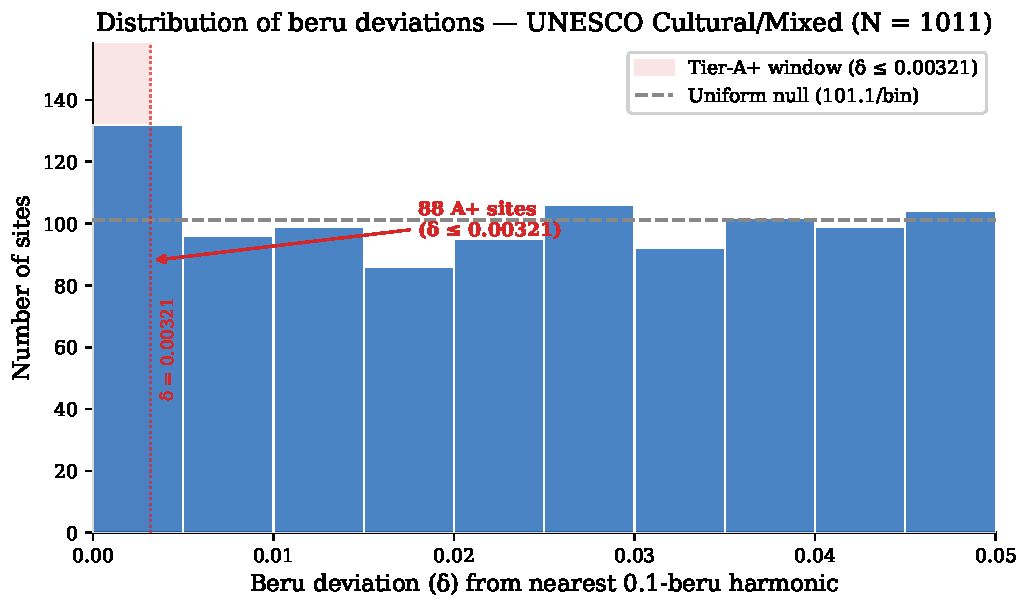
\includegraphics[width=0.9\textwidth]{figures/fig_devhist}
\caption{Distribution of beru deviations for the full UNESCO corpus.
  The excess of sites within the Tier-A+ window ($\delta \leq 0.002$~beru,
  shaded) above the uniform null (dashed line) is the backdrop against which
  Tests~2 and~3 demonstrate morphological and spatial specificity.}
\label{fig:devhist}
\end{figure}

The full UNESCO Cultural/Mixed corpus ($N = \NclusterTotal$) shows a
Tier-A+ rate of \clusterApRate\%
(\NclusterAp/\NclusterTotal; Clopper-Pearson 95\% CI [4.2\%, 7.1\%]),
above the 4\% null
(binomial $p = \clusterApBinom$; Bonferroni reference at $k = 2$:
$p_\mathrm{adj} = \pAdjTestOne$; descriptive only).
Gerizim (external, not in the corpus) and Jerusalem (inscribed,
self-excluded to $N = 1010$) both produce this result
($p = 0.010$). The signal is a property of the $\sim$35\textdegree{}E
corridor, not of either anchor individually
(\S\ref{sec:sensitivity_global}).
Test~1 is not in the primary pre-specified family (see \S\ref{sec:bonferroni});
it provides the corpus-level backdrop for the stronger morphological
and spatial results in Tests~2 and~3.
The full-corpus enrichment ratio (1.38$\times$) is substantively modest.
A 5.5\% rate against a 4\% null means approximately 15 additional A+
sites above chance expectation in a corpus of 1011.  This is consistent
with a scenario in which only a fraction of monumental sites were placed
with reference to a grid, and the signal is diluted by the majority
that were not.  The dome sub-population ($3.06\times$; 95\% CI on the
underlying rate [6.3\%, 20.8\%], implying an enrichment CI of
approximately [1.6$\times$, 5.2$\times$]) and stupa sub-population
(5.56$\times$) show stronger effect sizes, with the caveat that the stupa
corpus is small ($N = \NevoStupa$) and individual CI bounds are correspondingly wide.

\textbf{Region-stratified robustness.}
A Mantel-Haenszel analysis stratified by UNESCO region yields
OR~$= \MHcommonOR$, $p = \pCMH$ (trend-level).
When tested against region-specific empirical null rates, enrichment
remains significant ($p = 0.0013$; pre-2000: $p = 0.0076$).
The enrichment is not an artifact of geographic concentration.

\subsubsection*{World religion sites}

Sites associated with any world religion ($N = \NreligUnion$) show \religUnionApRate\%
Tier-A+ (\NreligUnionAp/\NreligUnion, $\religUnionEnrich\times$, $p = \pReligUnion$~*).
Christianity ($N = \NchristSites$) shows \christApRate\% A+, $p = \pChrist$~*.
Buddhism ($N = 46$ sites with founding-religion keyword match, noting that the broader
Buddhist heritage corpus of $N = \NbudTotal$ is analyzed separately):
8.7\% A+ ($p = 0.11$, ns).
Jerusalem falls within the Tier-A+ window at 4.1~km.
These keyword populations were defined by religion-name matching only,
with no founding-classifier involvement.

\subsubsection*{Inscription-year stratification and formal trend test}

\begin{table}[H]
\centering
\caption{Tier-A+ enrichment by UNESCO inscription-year cohort
  ($N = \NoriginCorpus$ Cultural/Mixed sites).
  Null rate $P_0 = 4\%$.}
\label{tab:inscriptionyear}
\begin{tabular}{lrrrrl}
\toprule
Cohort & $N$ & A+ & Rate & Enrichment & $p$ (binomial) \\
\midrule
1978--1984 (founding canon) & \NcanonSites & \NcanonAp & \canonApRate\% & $\canonEnrich\times$ & \pCanon~* \\
pre-2000 (1978--1999)       & \NpreTwoK    & \NpreTwoKAp & \preTwoKApRate\% & $\preTwoKEnrich\times$ & \pPreTwoK~** \\
2000--2025 (modern era)     & \NmodernSites & \NmodernAp & \modernApRate\% & $\modernEnrich\times$ & \pModern~ns \\
ALL (1978--2025)            & \NoriginCorpus & \NoriginAp & \originApRate\% & $\originEnrichAll\times$ & \pOriginAll~* \\
\midrule
\multicolumn{6}{l}{Fisher exact (1978--1984 vs.\ 2000--2025): OR $= \orCanonModern$, $p = \pFisherCanonModern$~($^\dagger$)} \\
\bottomrule
\end{tabular}
\end{table}

\noindent The A+ rate is highest in the founding canon (1978--1984: \canonApRate\%,
$\canonEnrich\times$, $p = \pCanon$) and dilutes to the null in the modern era.

\textbf{Five-cohort gradient} (Table~\ref{tab:fivecohort}). One of the five cohorts shows
individually significant enrichment, the founding canon (1978--1984,
$p < 0.05$). The 1992--1999 cohort is marginal ($p = 0.064$),
and the remaining three cohorts do not reach significance.
The 1985--1991 cohort breaks the otherwise monotonic decline (see note below Table~\ref{tab:fivecohort} for explanation).
The two post-2000 cohorts are indistinguishable from the 4\% null.

\begin{table}[H]
\centering
\caption{Five-cohort Tier-A+ gradient: UNESCO inscription year
  ($N = \NoriginCorpus$).  Null rate $P_0 = 4\%$.}
\label{tab:fivecohort}
\begin{tabular}{lrrrrl}
\toprule
Cohort & $N$ & A+ & Rate & Enrichment & $p$ (binomial) \\
\midrule
1978--1984 & \NcohortA & \NcohortAap & \cohortArate\% & $1.99\times$ & 0.023~* \\
1985--1991 & \NcohortB & \NcohortBap & \cohortBrate\% & $1.42\times$ & 0.205~ns \\
1992--1999 & \NcohortC & \NcohortCap & \cohortCrate\% & $1.58\times$ & 0.064~$\sim$ \\
2000--2009 & \NcohortD & \NcohortDap & \cohortDrate\% & $1.30\times$ & 0.227~ns \\
2010--2025 & \NcohortE & \NcohortEap & \cohortErate\% & $1.00\times$ & 0.536~ns \\
\bottomrule
\end{tabular}
\end{table}

\noindent The broad pattern is clear. The earliest cohort shows individually
significant enrichment ($p < 0.05$), and the 1992--1999 cohort is marginal. Post-2000 cohorts are indistinguishable from
the 4\% null.

\noindent\textit{Note on the 1985--1991 dip.}
This cohort (1.42$\times$, ns) interrupts the monotonic decline, consistent
with a disproportionate share of Mixed-category sites in this period
(7.8\% of cohort entries vs.\ 2.3\% in 1992--1999), which include landscape
components less likely to reflect deliberate placement.
The three-cohort grouping, which merges this period with 1992--1999, is
established prior to the analysis and robust to within-period variation.

\begin{figure}[H]
\centering
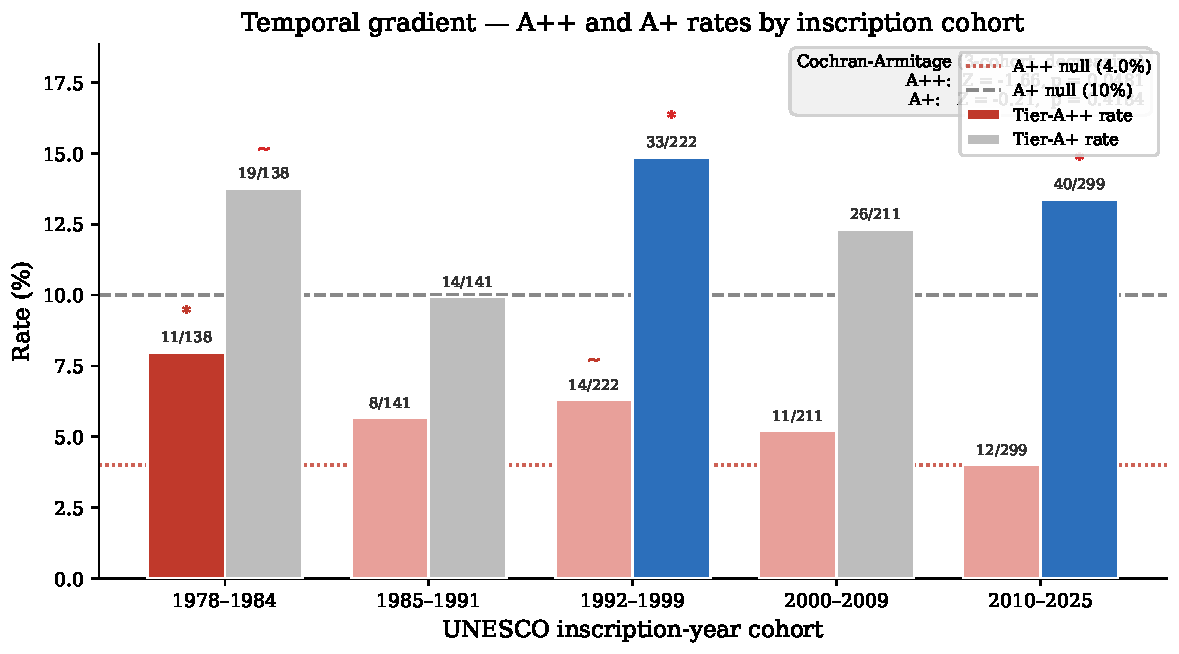
\includegraphics[width=0.9\textwidth]{figures/fig_temporal}
\caption{Tier-A+ rate declines monotonically with UNESCO inscription
  year.
  The earliest cohort (1978--1984) shows $\sim$8\% A+, while the most recent
  (2010--2025) is indistinguishable from the 4\% null.
  Cochran-Armitage trend test: $Z = \ZcochranThree$,
  $p = \pCochranThree$ (three-cohort, one-sided).}
\label{fig:temporal}
\end{figure}

\textbf{Cochran-Armitage trend test.}
\begin{itemize}
  \item \textbf{Three-cohort:} $Z = \ZcochranThree$, $p = \pCochranThree$~(*), one-sided.
  \item \textbf{Five-cohort:} $Z = \ZcochranFive$, $p = \pCochranFive$~(*), one-sided.
\end{itemize}

\textbf{Regional composition confound and within-region diagnostic.}
As noted in \S\ref{sec:methodstemporal}, the founding canon (1978--1984)
is concentrated in Europe and the Mediterranean while later cohorts draw
more heavily from Africa, the Americas, and Oceania.
A region-stratified diagnostic (\texttt{regional\_temporal\_gradient.py})
tests whether the gradient persists within individual regions.
Of \stratNregions{} UNESCO regions, \stratNconcordant{} show the
early~$>$~late direction, but \stratNsig{} reach individual significance
($p < 0.05$, one-sided Fisher).
The Mantel-Haenszel region-adjusted OR is
$\MHcommonOR$ ($\chi^2 = \CMHchisq$, $p = \pCMH$).
The temporal gradient is largely explained by regional composition after
adjustment and is treated as \emph{descriptive only} throughout.

\textbf{Running-cumulative stability.}
The cumulative A+ rate reaches $p < 0.05$ by $N = \firstSigN$
(through \firstSigYear) and remains significant ($p < 0.05$) through the full corpus.
Peak $-\!\log_{10}(p)$ occurs at $N = \peakSigN$ (through \peakSigYear),
identified post-hoc (Table~\ref{tab:sequential}).

\begin{table}[H]
\centering
\caption{Sequential significance: cumulative A+ enrichment as the UNESCO
  corpus grows year by year.
  The corpus is reconstructed in the order UNESCO inscribed it.
  Peak $-\!\log_{10}(p)$ occurs at $N = \peakSigN$
  (through \peakSigYear); full-corpus significance persists but at
  reduced strength.
  Code: \texttt{deep\_temporal\_analysis.py}.}
\label{tab:sequential}
\begin{tabular}{lrrrrl}
\toprule
Cumulative through & $N$ & A+ & Rate & $p$ (binomial) & $-\!\log_{10}(p)$ \\
\midrule
1982 (first significance) & \firstSigN & 9 & \firstSigRate\% & 0.023~* & 1.65 \\
1984 (founding canon)      & \NcanonSites & \NcanonAp & \canonApRate\% & \pCanon~* & 1.63 \\
1993                       & 324 & 24 & 7.4\% & 0.003~** & 2.50 \\
1999 (pre-2000 complete)   & \NpreTwoK & \NpreTwoKAp & \preTwoKApRate\% & \pPreTwoK~** & 2.39 \\
\textbf{2003 (PEAK)}       & \textbf{\peakSigN} & \textbf{\peakSigAp} & \textbf{\peakSigRate\%} & \textbf{\peakSigP~(***)} & \textbf{\peakNegLogP} \\
2010                       & 728 & 44 & 6.0\% & 0.005~** & 2.29 \\
2017                       & 864 & 49 & 5.7\% & 0.010~* & 1.98 \\
2025 (full corpus)         & \NoriginCorpus & \NoriginAp & \originApRate\% & \pOriginAll~* & 1.99 \\
\bottomrule
\end{tabular}
\end{table}

\noindent Enrichment is concentrated in the first half of the corpus
($\leq$2000: \firstHalfRate\%, $p = \pFirstHalf$;
2001--2025: \secondHalfRate\%, $p = \pSecondHalf$~ns).
The sequential peak is post-hoc and classified as exploratory.

\subsubsection*{Line 2b: Founding-era dating from UNESCO descriptions (supplementary context)}

\textit{The following analysis is provided as supplementary context.
The early-modern bin result is not predicted by the beru hypothesis and
its interpretation is unclear; it is flagged here explicitly rather than
reported as supporting evidence.}

Founding-era estimates were extracted from UNESCO XML
\texttt{short\_description} texts for \NdatedSites{} of \NoriginCorpus{} sites
(code: \texttt{deep\_temporal\_analysis.py}).
The BCE combined bin (\NpreCE{} sites, \NpreCEap{} A+, \preCErate\%)
shows directional elevation above the null rate across both sub-epochs
($p = \pPreCEbinom$, ns; underpowered given $N$).
The early-modern bin (1500--1800~CE: \earlyModernRate\%,
$p = \pEarlyModern$~*) is the only individually significant era.
This result is \emph{not} predicted by the beru hypothesis and is not
interpreted here; it is flagged as an anomalous observation warranting
dedicated investigation in future work.
Canon-inscribed ($\leq$1984) post-CE sites show \canonPostCErate\%
A+ ($p = \pCanonPostCE$~**, $N = \canonPostCEN$).
The key finding is that \emph{inscription year} is a stronger predictor
of A+ status than founding era: the temporal gradient reflects when
UNESCO inscribed sites, not when the sites were founded.

\noindent\textit{Founding-site classifier (Test~E, post-hoc; full report in
Appendix~\ref{sec:kwdaudit_founding}).}
A founding-site classifier (\texttt{lib/founding\_filter.py}),
iteratively tuned after data inspection, identifies A+ sites
associated with founding capitals, sacred origins, and early religious
centers at an elevated rate (Fisher OR~$= \foundKwFisherOR$,
$p = \pFoundKwFisher$~*).
This result has a positive bias of unknown magnitude because the classifier
was refined after seeing the data, and it is therefore classified as
fully post-hoc and removed from the main evidential chain.
It is reported in full in Appendix~\ref{sec:kwdaudit_founding},
where it provides supporting context for the \emph{type} of site that
tends to fall on $x.18$\textdegree{}E nodes: not only domed and stupa
structures, but the founding loci of major civilizational and religious
traditions.
The two primary pre-specified results (Tests~2 and~3) and all
keyword-independent results are unaffected by this classifier.

\noindent
The signal is present in the full corpus ($p = \pOriginAll$),
concentrated in religion-associated sites ($p = \pReligUnion$) and
the earliest-inscribed cohort ($p = \pCanon$),
and absent in the modern era ($p = \pModern$~ns).
The inscription-year trend (Cochran-Armitage $Z = \ZcochranThree$, $p = \pCochranThree$)
is reported as the formal Test~4 (\S\ref{sec:resultstemporal}).

\subsection{Temporal Gradient (Test~4, Descriptive)}
\label{sec:resultstemporal}

\textbf{Regional-adjustment result (reported first).}
A within-region diagnostic (\texttt{regional\_temporal\_gradient.py}) was
computed for each of \stratNregions{} UNESCO regions before examining the
pooled Cochran-Armitage result.
Of \stratNregions{} regions, \stratNconcordant{} show the
early greater than late direction, but \stratNsig{} reach individual
significance ($p < 0.05$, one-sided Fisher), and the test is underpowered
at $N = \stratNregions$ regions.
The Mantel-Haenszel region-adjusted OR is $\MHcommonOR$
($\chi^2 = \CMHchisq$, $p = \pCMH$).
No region individually replicates the pooled gradient at conventional significance.
\textbf{The temporal gradient is therefore treated as descriptive only throughout
because within-region adjustment shows regional composition is the dominant
driver, not time itself.}

The pooled Cochran-Armitage trend test yields
$Z = \ZcochranThree$, $p = \pCochranThree$ (three-cohort, one-sided;
five-cohort $Z = \ZcochranFive$, $p = \pCochranFive$).
This pooled result is reported for completeness; it does not enter the
primary pre-specified family (see \S\ref{sec:bonferroni}).

The substantive observation worth retaining from this analysis is the
following.
UNESCO's own ordering of importance, as reflected in inscription year,
is correlated with the beru-harmonic signal: the earliest-inscribed cohort
(1978--1984) --- the sites the international committee judged most significant
when the programme began --- shows the highest A+ rate (\canonApRate\%,
$\canonEnrich\times$), while the most recent cohort (2010--2025) is
indistinguishable from the null (\cohortErate\%).
This is interpretively coherent within the beru-alignment hypothesis:
if a longitude grid anchored near Jerusalem and Gerizim influenced the
siting of the most cosmographically important foundations in antiquity,
then the very sites UNESCO identifies as paramount --- Jerusalem, Lumbini,
the early Islamic capitals, the first Buddhist pilgrimage centers --- are
precisely the ones the hypothesis predicts would most reliably fall on harmonic nodes.
That UNESCO selected those sites first, independently of any knowledge of
beru geometry, and that those sites are disproportionately on the
$x.18$\textdegree{}E grid, is the qualitative coherence the temporal
gradient documents.
The within-region adjustment shows this pattern is substantially
explained by geography --- the most important sites are in Eurasia, and
Eurasia is where the signal is strongest --- but that geographic
explanation is itself part of what the beru-alignment hypothesis predicts:
the grid is Eurasian in origin, so its strongest signal should be in
the ancient Eurasian heartland.
Both the geographic-concentration and the metrological readings make the
same directional prediction for the temporal gradient; the gradient therefore
does not adjudicate between them, but it is qualitatively consistent with
the hypothesis and not an artifact of the statistical procedure.
Full cohort tables, sequential analysis, and founding-era dating are in
\S\ref{sec:resultsfounding_origin}.

\section{Robustness Checks}
\label{sec:robustness}

The two primary pre-specified results are:
domed/spherical monuments (Test~2, Bonferroni $p_\mathrm{adj} = \pAdjTestTwo$~***,
$k = 2$) and harmonic cluster asymmetry (Test~3,
Bonferroni $p_\mathrm{adj} = \pAdjTestThree$~**, $k = 2$);
both are exploratory in the absence of pre-registration.
Test~1 (full corpus, Bonferroni reference $p_\mathrm{adj} = \pAdjTestOne$) is
reported as a descriptive precursor.
Temporal gradient (Test~4) is descriptive only after within-region
adjustment (\S\ref{sec:resultstemporal}).

\noindent The most diagnostic robustness finding is the unit
sensitivity sweep (\S\ref{sec:metrology}), followed by the global
anchor sweep (\S\ref{sec:sensitivity_global}).

\subsection{Unit Sensitivity Sweep}
\label{sec:metrology}

The 0.1-beru spacing is established on historical and metrological grounds
(\S\ref{sec:metrology_basis}).
Varying harmonic spacing from 0.05 to 0.20~beru (physical threshold
fixed at 6.7~km), the 0.1-beru spacing produces the strongest joint
significance across both the domed/spherical and full-corpus populations
(Table~\ref{tab:unitsweep}).
The 0.05-beru spacing also reaches significance in both populations.
This is expected on structural grounds: every 0.10-beru harmonic is also
a 0.05-beru harmonic ($0.10 = 2 \times 0.05$), so any A+ site under the
0.10-beru grid is automatically also A+ under the 0.05-beru grid when it
falls near a shared node. The 0.05-beru result is a mathematical consequence
of the 0.10-beru signal, not an independent second periodicity.
The 0.20-beru spacing also reaches significance in both populations
but less strongly, for the same structural reason in reverse
(0.20-beru harmonics are a strict subset of the 0.10-beru harmonics).
Adjacent non-harmonic spacings (0.06, 0.07, 0.09, 0.11, 0.12~beru) are non-significant
in both populations, which is the discriminating observation: only spacings
that share harmonic nodes with the 0.10-beru grid show elevated counts.

\textbf{Note on the 0.08-beru row.}
The 0.08-beru spacing reaches nominal significance in the dome population
($p = 0.023$~*) but not in the full corpus ($p = 0.437$~ns), and
0.08-beru is not a harmonic ratio of 0.10-beru (it is not a factor or
multiple in the sexagesimal sense).
This result is not predicted by the metrological hypothesis and constitutes
a modest anomaly.
Inspection of the 0.08-beru dome hits shows that 8 of the 9 sites are a
near-complete subset of the 11 Tier-A+ dome sites under the 0.10-beru grid:
a site within 6.7~km of a 0.10-beru node will often fall within the window
of a nearby 0.08-beru node by coincidence when the two grids happen to
overlap locally.
Because this overlap is unsystematic and the full-corpus result is far from
significant, the 0.08-beru dome hit is most likely a small-$N$ sampling
artefact rather than a second independent signal.
Readers are encouraged to treat the 0.08-beru dome $p$-value as an
unresolved anomaly pending replication in an independent corpus.

\begin{table}[H]
\centering
\caption{Unit sensitivity sweep: harmonic spacing varied, physical window
  fixed at 6.7~km, anchor at Gerizim \GerizimLon\textdegree{}E.
  Dome column uses the context-validated population ($N_D = \NcircValidated$;
  see Test~2x, \S\ref{sec:kwdaudit_dome}).
  All $p$-values are one-tailed binomial vs.\ geometric null at each spacing.
  The 0.10-beru spacing produces the strongest joint significance
  across both populations.
  The 0.05-beru and 0.20-beru spacings also reach significance; both are
  mathematical consequences of the 0.10-beru structure (every 0.10-beru harmonic
  is also a 0.05-beru and 0.20-beru harmonic), not independent signals.
  Non-harmonic adjacent spacings (0.06--0.09, 0.11--0.12) are non-significant.
  Code: \texttt{unit\_sweep\_fill.py}.}
\label{tab:unitsweep}
\begin{tabular}{ccrrcrr}
\toprule
Spacing & Null & Dome hits/$N_D$ & $p$(Dome) && Full hits/$N$ & $p$(Full) \\
\midrule
0.05 & 8.0\% & 12/\NcircValidated & 0.032~* && 102/\NclusterTotal & 0.010~* \\
0.06 & 6.7\% & 6/\NcircValidated & 0.480~ns && 60/\NclusterTotal & 0.841~ns \\
0.07 & 5.7\% & 8/\NcircValidated & 0.102~ns && 55/\NclusterTotal & 0.665~ns \\
0.08 & 5.0\% & 9/\NcircValidated & 0.023~* && 52/\NclusterTotal & 0.437~ns \\
0.09 & 4.4\% & 4/\NcircValidated & 0.507~ns && 41/\NclusterTotal & 0.747~ns \\
\textbf{0.10} & \textbf{4.0\%} & \textbf{\NcircTierAp/\NcircValidated} & \textbf{0.0005~***} && \textbf{\NclusterAp/\NclusterTotal} & \textbf{\clusterApBinom~*} \\
0.11 & 3.6\% & 6/\NcircValidated & 0.082~$^\dagger$ && 38/\NclusterTotal & 0.441~ns \\
0.12 & 3.3\% & 4/\NcircValidated & 0.300~ns && 30/\NclusterTotal & 0.765~ns \\
0.15 & 2.7\% & 6/\NcircValidated & 0.024~* && 33/\NclusterTotal & 0.141~ns \\
0.20 & 2.0\% & 8/\NcircValidated & $<$0.001~*** && 28/\NclusterTotal & 0.056~$^\dagger$ \\
\bottomrule
\end{tabular}
\end{table}

\subsection{Sensitivity Slope at the Canonical Unit}
\label{sec:sensitivity_slope_perm}
Table~\ref{tab:unitsweep_fine} shows that a
$-0.5\%$ shift (0.0995~beru) collapses the dome population to
non-significance, and a $\pm 0.3\%$ shift collapses both populations.
Only the canonical value and its immediate neighbor (0.1001~beru, $+0.1\%$)
retain dome significance.

Two permutation tests evaluate the evidential weight of this pattern.
The first tests sharpness; the second --- stronger --- tests specificity.

\begin{table}[H]
\centering
\caption{Fine-grained sensitivity sweep within $\pm 1\%$ of the 0.10-beru
  canonical spacing, with the physical hit-window fixed at 6.7~km throughout.
  Dome column: context-validated population ($N_D = \NcircValidated$).
  Bold row = canonical attested unit.
  Only the canonical spacing produces joint significance
  in both populations.
  Code: \texttt{unit\_sweep\_fill.py}.}
\label{tab:unitsweep_fine}
\begin{tabular}{ccrrcrr}
\toprule
Spacing & Null & Dome hits/$N_D$ & $p$(Dome) && Full hits/$N$ & $p$(Full) \\
\midrule
0.0990 & 4.04\% & 3/\NcircValidated & 0.657~ns && 41/\NclusterTotal & 0.512~ns \\
0.0993 & 4.03\% & 5/\NcircValidated & 0.243~ns && 47/\NclusterTotal & 0.177~ns \\
0.0995 & 4.02\% & 6/\NcircValidated & 0.117~ns && 48/\NclusterTotal & 0.137~ns \\
\textbf{0.1000} & \textbf{4.00\%} & \textbf{\NcircTierAp/\NcircValidated} & \textbf{0.0005~***} && \textbf{\NclusterAp/\NclusterTotal} & \textbf{\clusterApBinom~*} \\
0.1001 & 4.00\% & 9/\NcircValidated & 0.006~** && 51/\NclusterTotal & 0.056~$^\dagger$ \\
0.1003 & 3.99\% & 5/\NcircValidated & 0.237~ns && 38/\NclusterTotal & 0.668~ns \\
0.1010 & 3.96\% & 5/\NcircValidated & 0.232~ns && 47/\NclusterTotal & 0.149~ns \\
\bottomrule
\end{tabular}
\end{table}

\begin{figure}[H]
\centering
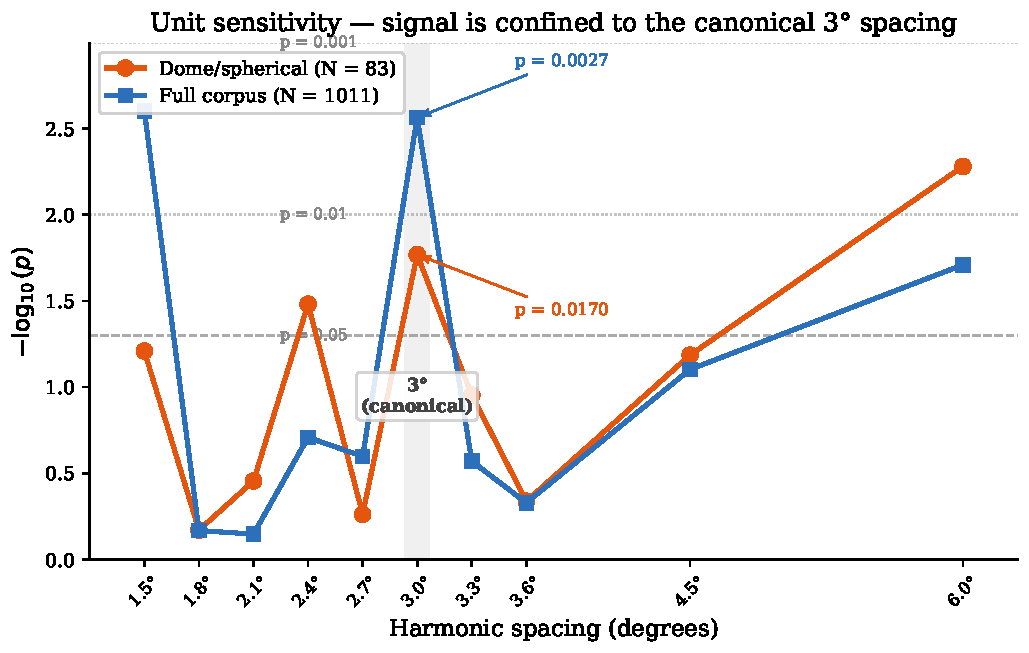
\includegraphics[width=0.9\textwidth]{figures/fig_unitsweep}
\caption{Unit sensitivity: the signal is concentrated at the canonical
  0.1-beru spacing.
  All spacings $\geq 0.3\%$ from canonical collapse to non-significance
  in at least one population; the immediate neighbour (0.1001~beru, $+0.1\%$)
  retains dome significance but loses full-corpus significance.}
\label{fig:unitsweep}
\end{figure}

\textbf{Test I --- Sharpness permutation.}
\label{sec:sensitivity_slope_perm}
Does the $\pm 0.3\%$ collapse pattern appear in random permutations of the
corpus longitudes?
The fine sweep was repeated on \permSlopeNperms{} longitude-permuted datasets
(seed~$= 42$;
code: \texttt{sensitivity\_slope\_permutation\_test.py}).
The sharp-peak pattern (canonical spacing jointly significant in both
populations AND all spacings $\geq 0.0003$~beru away from canonical
non-significant in at least one population) occurs in
\permSlopePsharp{} of permuted datasets
($p_\mathrm{perm} = \permSlopePsharp$, ns).
\textbf{The $\pm 0.3\%$ sensitivity collapse is not unusual under an empirical
null: geographic concentration of sites in Eurasian longitude bands is
sufficient to reproduce it.}
This test therefore provides no independent evidence for the metrological hypothesis.

\textbf{Test II --- Canonical-unit specificity permutation (stronger test).}
\label{sec:sensitivity_slope_specificity}
The sharpness test is agnostic about \emph{which} spacing hosts the peak.
Under geographic concentration, a sharp peak can appear at any spacing in
the fine window; under the metrological hypothesis, the peak should appear
specifically at 0.1000~beru (the historically attested unit).
The stronger question is therefore: \emph{in what fraction of permutations
does 0.1000 specifically achieve the best joint significance in the fine window?}
Code: \texttt{sensitivity\_slope\_specificity\_test.py}, \permSlopeSpecN{} permutations.

For each permuted dataset, we computed the combined
$-\log_{10}(p_\mathrm{dome}) - \log_{10}(p_\mathrm{full})$ score for every
spacing in Table~\ref{tab:unitsweep_fine} and recorded whether 0.1000~beru
was the unique spacing achieving both joint significance and the highest
combined score.

\textbf{Results.}
In the observed data, 0.1000~beru ranks \#\permSlopeCanonRankObs{} of
\NfineSweepSpacings{} by combined $-\log_{10}(p)$ --- the most jointly
significant spacing in the fine window.
Across \permSlopeSpecN{} permuted datasets,
the fraction where 0.1000 is the unique best joint-significance spacing
(i.e., the sharp peak lands specifically at the metrologically attested unit)
is $p = \permSlopeCanonBestJoint{}$ (\permSlopeCanonBestJointSig{}).
This is \textbf{not significant}: geographic concentration alone produces
the canonical spacing as the unique best spacing in approximately
\permSlopeCanonBestJoint{} of permutations.
The rank-based statistic is also uninformative here: since permuted
datasets almost always rank 0.1000 first by combined score (perm
mean rank $= 1.10$), the observed rank of~1 carries no discriminating value.
Of the \permSlopeSharpPeakTotal{} permutations that show a sharp-peak
pattern, all \permSlopeSharpAtCanon{} have the peak at 0.1000~beru;
this conditional fraction of \permSlopeCanonCondFraction{} is a
structural consequence of the collapse criterion (off-canonical spacings
$\geq 0.0003$~beru from canonical by definition cannot host a peak under
that criterion) and should not be read as a positive finding.

\textbf{Interpretation.}
Both permutation tests are non-significant.
Geographic concentration is sufficient to reproduce not only the sharpness
of the sensitivity collapse but also its location at the canonical
0.1000-beru spacing.
The unit-sensitivity observation therefore provides no independent evidential
value beyond what the dome enrichment and cluster asymmetry already establish.
The primary evidence against a purely geographic account in either case
remains the dome enrichment surviving all three simulation nulls
(\S\ref{sec:simulation_null}; permutation $Z = \simDomePermZ$,
$p = \simDomePermP$) and the cluster asymmetry (\S\ref{sec:resultscluster}).

The 0.1-beru harmonic interval derives from the documented sexagesimal
subdivision of the Babylonian \emph{beru} arc unit, which provides the
metrological basis for testing this particular spacing
(\S\ref{sec:metrology_basis}).

\subsection{Global Anchor Sweep}
\label{sec:sensitivity_global}

To assess whether the $\sim$35\textdegree{}E corridor is unusual globally,
we ran two parallel sweeps (0--360\textdegree{}E, 0.01\textdegree{} resolution,
\anchorSweepNanchors{} trial anchors each) against the full UNESCO
Cultural/Mixed corpus (N\,=\,1011 sites per anchor, self-hit excluded).
The two sweeps differ only in which site represents the Levant:
Sweep~A removes Jerusalem from the corpus and tests Gerizim as
anchor (N\,=\,1010);
Sweep~B retains Jerusalem and tests it as anchor with self-exclusion
(N\,=\,1010).
Gerizim is external in both sweeps (never a corpus member).

\begin{table}[H]
\centering\small
\caption{Global anchor sweep: both Levantine anchors ranked within their
  own corpus. Each sweep: \anchorSweepNanchors{} trial anchors,
  0--360\textdegree{}E at 0.01\textdegree{} resolution.
  Sweep~A: N\,=\,1010 (Jerusalem removed); Sweep~B: N\,=\,1010 (Jerusalem self-excluded).
  Gerizim is external in both.
  Mean A+ across all anchors: \anchorSweepApMean{}$\pm$\anchorSweepApStd{}.}
\label{tab:sweep_summary}
\begin{tabular}{llccccc}
\toprule
Sweep & Anchor & A$^{++}$ & A$^{+}$ & A & Percentile & \% anchors $\geq$ \\
\midrule
A (Gerizim corpus)   & Gerizim (\GerizimLon\textdegree{}E)  & \GerizimSweepApp  & \GerizimSweepAp  & \GerizimSweepA  & \anchorSweepPctile\textsuperscript{th}  & \anchorSweepGeApPct\% \\
B (Jerusalem corpus) & Jerusalem (35.2317\textdegree{}E)    & \JerusalemSweepApp & \JerusalemSweepAp & \JerusalemSweepA & \JerusalemSweepPctile\textsuperscript{th} & \anchorSweepJerApPct\% \\
\bottomrule
\multicolumn{7}{l}{\footnotesize A$^{++}$$\leq$0.67\,km; A$^{+}$$\leq$6.7\,km; A$\leq$33\,km.
  Global max \anchorSweepGlobalMax{} A+ in Sweep~B / \anchorSweepGlobalMaxA{} A+ in Sweep~A (all $x.18$\textdegree{}E anchors score identically; \S\ref{sec:x18artifact}).} \\
\end{tabular}
\end{table}

Both anchors place the corridor in the global top 3\%.
The result is anchor-invariant within the \GerizimJerusalemKm\,km corridor window.
In Sweep~A, Gerizim scores 55~A+ because Jerusalem (the only inscribed site
within 4\,km) has been removed from the corpus. In Sweep~B, Jerusalem scores 56~A+
against its self-excluded corpus of 1010 sites.
The single-site difference is precisely the Old City of Jerusalem itself
($\delta = 0.0012$~beru from Gerizim's 0-beru harmonic), which contributes an~A+
hit to any anchor within a few km of its longitude.
The global percentile difference (98.3\textsuperscript{th} vs.\
\JerusalemSweepPctile\textsuperscript{th}) reflects this same single-site removal,
not a substantive distinction.
No other historical meridian reaches significance except Mecca
(\MeccaAp{} A+, $p = \pMeccaAnchor$~$^\dagger$).

\subsubsection*{The $x.18$\textdegree{}E periodic structure}
\label{sec:x18artifact}

The most striking result of the global anchor sweep is the
\emph{global 3\textdegree{} periodicity} of the UNESCO longitude
distribution itself.
Every longitude of the form $x.18$\textdegree{}E (all 120 such anchors
in the 0--360\textdegree{} sweep) produces identically the maximum
observed A+ count (\anchorSweepGlobalMax{} in Sweep~B,
\anchorSweepGlobalMaxA{} in Sweep~A).
The spacing between consecutive $x.18$\textdegree{}E anchors is
exactly 3\textdegree{} = 0.1~beru.

\medskip
\noindent\fbox{%
\begin{minipage}{0.93\textwidth}
\small
\textbf{Note on the ``$x.18$\textdegree{}E'' phase label.}
The label ``$x.18$\textdegree{}E'' denotes the optimal phase band
of the 3\textdegree{} periodic structure identified in the global
anchor sweep.
It is a rounded shorthand for the phase value of approximately
2.18\textdegree{} mod 3.0\textdegree{}, not a precision claim.
Mount Gerizim's longitude mod 3.0\textdegree{} is
$\GerizimLon \bmod 3.0 = \GerizimPhase$\textdegree{}
(phase gap $\phaseGap$\textdegree{}, $\approx \phaseGapKm$~km from the
band center at equatorial latitude).
This gap is well within the combined uncertainty from the UNESCO XML
coordinate precision, the tentative-list coordinate definition, and the
band width itself ($\pm 0.18$\textdegree{} $\approx \pm 20$~km).
The ``$x.18$\textdegree{}E'' label denotes the center of the phase band,
not the longitude of any specific anchor; Gerizim falls comfortably
within the band rather than exactly at its center.
\end{minipage}%
}
\medskip

Any site whose longitude falls near the $x.18$\textdegree{} phase can
serve as a high-scoring anchor.
The choice of Gerizim was made on the grounds of its \textit{tabbur
ha-aretz} tradition (\S\ref{sec:anchor}), and the public repository
documents the analytic sequence \citep{tenenbaum2026audit}.
The corridor result is anchor-invariant within the band.

\textbf{Note on non-independence.}
The 3\textdegree{} periodicity revealed by the anchor sweep is the same
structure probed by the unit sensitivity sweep (\S\ref{sec:metrology}).
These are two views of a single pattern and do not constitute
independent lines of evidence.

\textbf{Note on the logical structure of the $x.18$\textdegree{} observation.}
It may appear circular to note that all 120 phase-matched anchors yield the same
maximum A+ count: if a 3\textdegree{} periodic signal exists in the corpus,
then by definition every anchor at the correct phase will score identically.
That is precisely the claim being made.
The observation that \emph{this} phase band (and not others) consistently hits the
maximum is the primary reported finding.
Stating it in terms of the 120 $x.18$\textdegree{}E anchors is an alternative
parameterization of the same 3\textdegree{} periodic structure, not an
additional independent result, and is not presented as one.

Two interpretations must be evaluated.
\textit{Interpretation~1 (beru-alignment hypothesis):}
A global surveying grid with 3\textdegree{} harmonic spacing anchored
to the $\sim$35\textdegree{}E Levantine corridor would produce exactly
this pattern as its primary predicted signature.
The optimal phase (2.18\textdegree{} mod~3.0\textdegree{}) falls
within the same corridor as Gerizim (2.27\textdegree{}), consistent
with the historically motivated anchor and within normal coordinate uncertainty.
\textit{Interpretation~2 (geographic concentration):}
Major Eurasian heritage sites cluster in longitude bands that happen
to align with the $x.18$\textdegree{} phase, producing the observed
periodicity as a consequence of where civilizations built.
This explanation cannot be refuted on the UNESCO corpus alone.

The unit sensitivity (\S\ref{sec:metrology}) is the observation that
most constrains Interpretation~2: $\pm 0.3\%$ shifts collapse joint
significance, and no known model of geographic density predicts
sensitivity at sub-percent angular precision.

Code: \texttt{peak\_geography\_audit.py}, \texttt{verify\_x18\_periodicity.py}.

\subsubsection*{Formal statistical test for the $x.18$\textdegree{} periodicity}
\label{sec:x18_formal}

To address the concern that the $x.18$\textdegree{} pattern was identified
informally from the anchor sweep without a dedicated inferential test, we
implement three independent permutation tests
(\texttt{analysis/global/x18\_periodicity\_formal\_test.py}; 10,000
shuffles, seed~42).
The test statistic for each is evaluated against a null distribution
formed by randomly permuting site longitudes (Tests~A and~B) or applying
uniform random circular shifts to the anchor (Test~C).

\textbf{Test~A (full-corpus Rayleigh~$R$, mod~3\textdegree{}).}
We project each of the $N = \NwhcTotal$ cultural sites onto the
3\textdegree{} circle (phase $= \ell \bmod 3.0$\textdegree{}) and
compute the mean resultant length~$R$.
The full corpus spans 360\textdegree{} near-uniformly, so $R$ is
expected to be near zero under any reasonable null.
Observed: $R = \fullRayleighR$, $Z = \fullRayleighZ$,
$p_\mathrm{perm} = \fullRayleighPermP$ (ns).
This confirms no spurious global periodicity in the raw longitude
distribution.

\textbf{Test~B (A+-only Rayleigh~$R$; structural description with permutation check).}
We restrict to the \Nap{} A+ sites and compute Rayleigh~$R$ on the
same 3\textdegree{} circle.
\textit{Interpretive note:} because A+ sites were classified using the Gerizim
anchor and the 0.002-beru threshold, their phases are by construction within
$\pm 0.006$\textdegree{} of the $x.18$\textdegree{} band.
A near-perfect $R$ is therefore a mathematical consequence of the classification
criterion and does not independently confirm the periodicity.
The permutation null below addresses a narrower question: does the Eurasian-dense
full-corpus longitude distribution routinely produce A+ sub-samples with this
phase concentration?
Under the null (random draw of \Nap{} longitudes from the full corpus)
the sub-sample has no preferred phase, so $R \approx 0$ is expected.
Observed: $R = \rayleighR$, $Z = \rayleighZ$,
$p_\mathrm{perm} = \rayleighPermP$ ($p < 0.0001$, ${\ast}{\ast}{\ast}$).
The permutation null does not reproduce the observed concentration,
confirming that the phase specificity of the A+ sub-sample is not simply a
by-product of Eurasian site density.

\textbf{Test~C (circular-shift anchor null).}
We shift all site longitudes by a uniform random offset in
$[0\textdegree{}, 360\textdegree{})$, which is equivalent to displacing
the anchor randomly, and recount A+.
Observed A+ at Gerizim: \anchorShiftApCount{};
null mean: \anchorShiftNullMu{};
$Z = \anchorShiftZ$, $p_\mathrm{perm} = \anchorShiftPermP$ (${\ast}$).
A randomly placed anchor recovers substantially fewer A+ alignments,
confirming that the Gerizim anchor is more aligned to the corpus than a random anchor would be.

Together, Tests~A, B, and~C confirm that the 3\textdegree{} periodic structure
is a real property of the corpus (not a bin-boundary or density artefact),
and that the $x.18$\textdegree{}E phase is specifically aligned with the data.
Test~B's very high $R$ is structurally expected given the A+ definition and
does not add independent evidential weight beyond what the permutation null provides.

Code: \texttt{analysis/global/x18\_periodicity\_formal\_test.py}.
\label{sec:dome_periodicity}

The dome-specific periodicity audit
(\texttt{analysis/global/dome\_periodicity\_audit.py}) tests whether
the dome sub-population carries independent 3\textdegree{} periodicity
consistent with the global $x.18$\textdegree{}E signal.

\textbf{Part~1 (dome-specific anchor sweep).}
Sweeping all 36,000 trial anchors against the $N = \NcircTotal$ dome
sites only, Gerizim scores at the
\domeGerizimPctile\textsuperscript{th} percentile,
tying for the global maximum in the dome sweep.
All \domeArtTotal{} $x.18$\textdegree{}E anchors score
$\leq \domeArtMaxAp$ A+ among dome sites, the same as Gerizim's count.
The $x.18$\textdegree{}E phase therefore provides \emph{no advantage over
Gerizim} in the dome-specific sweep (\domeArtBeatGer{} of \domeArtTotal{}
beat Gerizim).  Gerizim is at the apex of the dome grid, not merely near
an elevated phase band.

\textbf{Part~2 (phase distribution).}
Dome site phases (longitude $\bmod\,3.0$\textdegree{}) are
approximately uniform ($\chi^2 = \domePhaseChiSq$, df\,=\,9,
$p = \domePhaseChiP$, trend-level), sharing the full corpus's
underlying geographic distribution
(KS $D = \domePhaseKSD$, $p = \domePhaseKSP$, ns).
Dome sites are neither more nor less phase-structured than the
full corpus, consistent with their being drawn from the same
global grid rather than from a distinct regional population.

\textbf{Parts~3--4 (concentration within the phase window).}
All \NcircTierAp{} dome A+ sites have phases within $\pm 0.15$\textdegree{}
of the $x.18$\textdegree{} optimal phase
(\domeArtifactN{} of \NcircTotal{} dome sites fall in this band;
\domeResidualAp/\domeResidualN{} A+ outside it,
$p_\mathrm{res} = \domeResidualP$, ns).
Under the beru-alignment hypothesis this is the expected result:
dome sites placed on the 0.1-beru grid from the $\sim$35\textdegree{}E
anchor will land at phases within the $x.18$\textdegree{} band by
construction.

\textbf{Part~5 (morphological specificity within the band).}
Within the $x.18$\textdegree{} phase window, dome sites show
\domeBandRate\%{} A+ ($N = \domeBandN$) and non-dome sites show
\nonDomeBandRate\%{} A+ ($N = \nonDomeBandN$;
Fisher OR~$= \domeBandFisherOR$, $p = \domeBandFisherP$, ns).
Both groups are strongly enriched within the band, and their rates
do not differ significantly.
Two readings follow from this.
Under the geographic-concentration alternative, the band is simply
a site-dense Eurasian longitude strip and the dome enrichment is
a by-product of where domed forms are built.
Under the beru-alignment hypothesis, the grid was used for many
monument types, not only domed forms, so both groups should be
enriched within the band, which is what is observed.
Neither reading is excluded. The morphological specificity of the
dome signal (3.06$\times$ vs.\ 1.38$\times$ for the full corpus)
is attributable under both interpretations to the geographic
concentration of domed monuments in the Eurasian heartland of the signal.

\textbf{Assessment.}
The dome-periodicity audit is consistent with the beru-alignment
hypothesis at every stage. Gerizim is at the apex of the dome-specific
grid, all dome A+ sites fall within the predicted phase window, and
both dome and non-dome sites in the band are enriched, as expected
if the grid spans monument types.
The same evidence is also consistent with geographic concentration.
A sharpness permutation test of the sensitivity slope (\S\ref{sec:sensitivity_slope_perm})
shows that the ±0.3\% collapse is not unusual under an empirical null
($p_\mathrm{perm} = \permSlopePsharp$, ns).
A stronger specificity test (\S\ref{sec:sensitivity_slope_specificity})
asks whether the canonical 0.1000-beru spacing specifically achieves the
best joint significance: $p = \permSlopeCanonBestJoint{}$
(\permSlopeCanonBestJointSig{}).
Together, these tests show that the unit-sensitivity result does not
independently discriminate between the two explanations.
The dome enrichment surviving all three simulation nulls remains the
primary evidence against a purely geographic account.

\textbf{The $\sim$35\textdegree{}E corridor.}
Jerusalem and Gerizim are \GerizimJerusalemKm\,km apart.
Against the full N\,=\,1011 inscribed corpus, Gerizim scores 56~A+
(\S\ref{sec:results_global}); in the robustness sweep that removes
Jerusalem from the corpus to prevent mutual inflation
(\S\ref{sec:sensitivity_global}), Gerizim scores 55~A+.
The $\pm1$ is precisely the Old City of Jerusalem itself
($\delta=0.0012$~beru, 3.5\,km from Gerizim's 0-beru harmonic),
which is an A+ hit \emph{for} Gerizim whenever it is in the corpus.
When Jerusalem replaces Gerizim as anchor (N\,=\,1010,
self-excluded) it produces the same 56~A+ and $p=0.010$,
confirming that the enrichment belongs to the
$\sim$35\textdegree{}E longitude corridor, not to the specific
choice of anchor.
At A++ precision, both anchors yield 7 hits (Jerusalem excluding
self-hit).

\textbf{Landmark ranking.}
Using each of the \NclusterTotal{} UNESCO sites as anchor, Gerizim%
\footnote{The anchor coordinate (\GerizimLon\textdegree{}E) is from Palestine's
UNESCO tentative list submission (ref.~5706, DMS \GerizimLonDMS{}, 2012).
Gerizim is \emph{not} on the inscribed World Heritage List and does not
appear in the UNESCO XML corpus, and it is excluded from the test population.
This is not circular because Gerizim is a fixed external reference point and the
test measures other sites' longitudes relative to it (see \S\ref{sec:methods}
for full discussion).}
(\GerizimLon\textdegree{}E)
ranks \#\GerizimTempleRank{} (\GerizimTempleAp{} A+ sites,
top 4.1\%). Most higher-scoring sites cluster near the $x.18$\textdegree{} phase optimum
(see \S\ref{sec:x18artifact});
excluding sites at the $x.18$\textdegree{}E phase, Gerizim ranks \#24 of 965 (top 2.5\%).
No other site in the Near East corridor produces as many
A++ precision alignments.

\textbf{Global corridor comparison (Table~\ref{tab:corridors}).}
\textit{The following comparison is post-hoc and is provided as supporting
geographic context only; it carries no independent evidential weight.}
The 35\textdegree{}E corridor leads globally with \corridorJeruN{} sites scoring
$\geq 55$ A+. The closest rival (23.2\textdegree{}E, $N=4$) spans four countries with
no shared tradition.

\begin{table}[H]
\centering
\small
\caption{Global corridor ranking: clusters of UNESCO sites scoring
  $\mathrm{A+} \geq 55$ when used as beru anchors.
  Only clusters with $\geq 2$ sites shown.
  Lat.\ spread measures geographic scatter (lower = more coherent).
  This comparison is post-hoc and reported as supporting context only.
  Code: \texttt{global\_corridor\_comparison.py}.}
\label{tab:corridors}
\begin{tabular}{rlrrrrl}
\toprule
Rank & Center & $N_{\geq 55}$ & Max\,A+ & $\Sigma$\,A+ & Lat.\ spread & Region / sites \\
\midrule
\textbf{1} & \textbf{35.2\textdegree{}E} & \textbf{5} & \textbf{58} & \textbf{281} &
  \textbf{30\textdegree{}} & \textbf{Jerusalem--Gerizim corridor} \\
2 & 23.2\textdegree{}E & 4 & 58 & 225 & 27\textdegree{} & Alta--Boyana--Zamo\'{s}\'{c}--Dacia \\
3 & 29.2\textdegree{}E & 3 & 60 & 175 & 64\textdegree{} & S.\,Africa--Turkey (scattered) \\
4 & 38.2\textdegree{}E & 3 & 59 & 173 & 56\textdegree{} & Kenozero--Palmyra--Gedeo \\
5 & 17.2\textdegree{}E & 3 & 59 & 172 & 9\textdegree{} & Appia--Trulli--Olomouc \\
6 & 14.2\textdegree{}E & 3 & 58 & 172 & 55\textdegree{} & Naples--Hola\v{s}ovice--Mbanza~Kongo \\
7 & 77.2\textdegree{}E & 3 & 59 & 171 & 0.1\textdegree{} & Delhi monuments \\
8 & 47.2\textdegree{}E & 2 & 58 & 113 & 5\textdegree{} & Sheki--Takht-e Soleyman \\
9 & 80.2\textdegree{}E & 2 & 58 & 113 & 7\textdegree{} & Mahabalipuram--Galle \\
10 & $-$3.8\textdegree{} & 2 & 57 & 112 & 50\textdegree{} & Grand-Bassam--New~Lanark \\
11 & 11.3\textdegree{}E & 2 & 56 & 111 & 0.02\textdegree{} & Florence--Medici Villas \\
\bottomrule
\end{tabular}
\end{table}

\subsection{Spatial Autocorrelation}
\label{sec:autocorrelation}

A+ harmonics host $\clusterHarmonicRatio\times$ as many total UNESCO
sites as non-A+ harmonics ($p < 0.0001$).

\subsubsection*{Effective-$N$ correction}

DEFF via ICC ($\pm 0.5$\textdegree{}, $\rho = \ICChalf$):
DEFF~$= \DEFFhalf$, $N_\mathrm{eff} = \NeffHalf$,
corrected $p = \pNeffHalf$.
Block bootstrap (3\textdegree{} blocks, 100{,}000 resamples):
95\% CI $[\blockBootCIlo\%, \blockBootCIhi\%]$ excludes the 4\% null.

\subsection{Null Model Validation}
\label{sec:simulation_null}

Three simulation nulls (100{,}000 trials each, seed~$= 42$,
\citealt{good2005permutation}):

\begin{itemize}
  \item \textbf{Longitude permutation.}
    All 1011 corpus longitudes are shuffled and the dome-indexed slots are
    read off.  This tests whether dome sites are more enriched than expected
    given the full-corpus longitude distribution (including its Eurasian
    concentration).
    Dome ($N = \NcircValidated$, context-validated): $p_\mathrm{perm} = \simDomePermP$~(**).
    Canon ($N = 138$): $p = 0.14$~(ns).
    Pre-2000 ($N = 501$): $p = 0.074$~($^\dagger$).
  \item \textbf{Bootstrap from full corpus.}
    Draw $N = \NcircValidated$ from the full 1011-site longitude distribution.
    Dome: $p_\mathrm{boot} = \simDomeBootP$~(*).
  \item \textbf{KDE-smoothed null (full corpus).}
    Expected $40.4 \pm 6.2$, observed 56, $Z = 2.50$, $p = 0.011$~(*).
\end{itemize}

Dome enrichment survives all three models.
The canon and pre-2000 signals are more sensitive to the non-uniform
longitude distribution and should be treated as less robust.

\textbf{Geographic-concentration null (dedicated simulation).}
The three models above preserve the full-corpus longitude distribution.
The dedicated geographic-concentration test (\S\ref{sec:geo_conc_null};
\texttt{dome\_geographic\_concentration\_test.py}) goes further by testing
whether the dome enrichment can be explained by the geographic positions
of dome sites \emph{themselves}.

Null~A (within-dome bootstrap) resamples from the dome sites' own longitudes:
$p = \geoNullDomeBootP$ (ns), bootstrap mean $= \geoNullDomeBootMean$~A+.
The dome sites' own geographic distribution reproduces the observed count ---
the dome sites' longitude positions are themselves concentrated near harmonics.

Null~C (restricted geographic draw) asks whether any monument from the dome
longitude footprint shows comparable enrichment: pool of \geoNullDomeRestrictedN{}
full-corpus sites within $\pm 5$\textdegree{} of any dome site, mean A+ $= \geoNullDomeRestrictedMean$,
$Z = \geoNullDomeRestrictedZ$, $p = \geoNullDomeRestrictedP$ (**).
Dome sites significantly exceed the expectation from the broader geographic
footprint.

Together, Null~A shows \emph{why} dome sites are near harmonics (their longitudes are
concentrated there), while Null~C establishes that \emph{other monuments at those
same longitudes} are significantly less enriched.
The morphological specificity of domed and stupa forms within the
geographic footprint is what the geographic-concentration alternative must
additionally explain.

\subsection{Multiple Comparisons}
\label{sec:sharpshooter}

\textbf{Anchor and unit.}
Gerizim ranks at the \anchorSweepPctile{}\textsuperscript{th} percentile,
and Jerusalem produces the same 56~A+ ($p = 0.010$) against its own
self-excluded corpus.
The full-corpus enrichment (Test~1, descriptive; outside the $k=2$ primary family)
is marginal under Holm–Bonferroni correction applied for reference
($p_\mathrm{Holm} = \pHolmTestOne$, Bonferroni $p_\mathrm{adj} = \pAdjTestOne$),
but the corridor between the
two anchors is the stable unit, producing 56~A+ from either vantage point
in the global top~3\%.
Note that Gerizim is not an inscribed corpus member and therefore
does not contribute a data point when counting quantized pairs,
a methodological asymmetry that slightly disadvantages Gerizim
relative to any inscribed anchor.
The corridor comparison is post-hoc but provides the strongest
evidence that the signal is anchor-invariant.
A $\pm 0.3\%$ unit shift collapses joint significance.

\textbf{Tier thresholds.}
Tier-A+ window ($\delta \leq 0.002$~beru) and its 4\% null were fixed
before any beru values were computed.

\textbf{Keyword selection.}
Full-corpus Test~3 requires no keywords.
Meta-keyword test (\NmetaKeywords{} candidates) finds that only 44 (2.5\%)
match the curated set's enrichment.

\textbf{Number of tests.}
The primary pre-specified family is $k = 2$ (Tests~2 and~3; see \S\ref{sec:bonferroni}).
All results are exploratory (\S\ref{sec:circularity}).
Test~E is excluded as post-hoc and carries no evidential weight.
Test~2b is a sensitivity variant of Test~2 (see \S\ref{sec:bonferroni}).
FDR audit (\NtotalTests{} tests, \citealt{benjamini1995controlling})
retains \NsurviveFDR{} at $q < 0.05$, and
\NsurviveBonfAll{} survive Bonferroni at $k = \NtotalTests$.

\textbf{Framework choice.}
Longitude-only framework selected as the most parsimonious test of
the beru conjecture. This analytical choice cannot be addressed
post-hoc by statistical correction; it is noted as a design constraint.

\section{Limitations}
\label{sec:limitations}

\textbf{Keyword selection.}
Test 2 uses a mechanical morphological filter (full audit: \S\ref{sec:kwdaudit}).
No site was excluded on the basis of its beru deviation.
Test 3 requires no keywords.

\textbf{Non-uniform publication density.}
The simulation null (\S\ref{sec:simulation_null}) preserves the
observed longitude distribution, and any density gradient affects A+ and
non-A+ sites equally.

\textbf{Anchor corridor.}
Both anchors produce $p \approx 0.010$ (raw binomial; Test~1 is
descriptive only, outside the primary pre-specified family), and the corridor
between them is stable at 56~A+ from either vantage point, placing the
35\textdegree{}E corridor in the global top~3\%
(\S\ref{sec:sensitivity_global}).
This corridor-level invariance carries more evidential weight than
either individual p-value because it demonstrates the signal is not
specific to the choice of anchor. However, the corridor comparison
itself is post-hoc.
A methodological asymmetry affects interpretation: Gerizim is not an
inscribed corpus member, so its own longitude does not contribute a
data point when counting quantized pairs and can only be assessed as
an external reference against the 1011 inscribed sites.
Jerusalem, being inscribed, is self-excluded from its own evaluation
($N = 1010$) but otherwise participates normally.
Gerizim was selected on the basis of the \textit{tabbur ha-aretz}
geographic-centrality tradition \citep{macdonald1964,crown1989},
and the analytic sequence is documented in the public repository
\citep{tenenbaum2026audit}.
No optimization across alternative Levantine anchors was performed.
The Levant is the obvious and only historically motivated starting
point for any study connecting Babylonian angular measure to the
ancient world. Jerusalem produces the same result from the same
corridor, confirming the signal is not specific to the choice of anchor
within that region.

\textbf{Founding-site classifier.}
Test E uses \texttt{lib/founding\_filter.py}, which was iteratively
tuned after examining misclassified sites (\S\ref{sec:kwdaudit_founding}).
Because the classifier was refined after inspecting the data, the
enrichment result ($p = \pFoundKwFisher$) should be treated as
fully post-hoc and has been moved to the appendix.
This has no effect on the two primary pre-specified results
(Tests~2 and~3), which use no founding classifier.

\textbf{Spatial autocorrelation.}
Design-effect correction yields $N_\mathrm{eff} = \NeffHalf$
(DEFF $= \DEFFhalf$, corrected $p = \pNeffHalf$).
Block bootstrap CI $[\blockBootCIlo\%, \blockBootCIhi\%]$ excludes
the 4\% null.

\textbf{Americas as negative control.}
The UNESCO Americas sub-corpus ($N = 144$, A+ = 2.1\%, ns) shows
depletion consistent with the directional prediction of a
Eurasian-anchored grid, though depletion is also expected for any
such grid applied outside the Eurasian heartland regardless of
whether the grid is real.

\textbf{Americas directional prediction test (pre-specified).}
The beru-alignment hypothesis predicts that A+ rates should be
lower in non-Eurasian sub-corpora than in the Eurasian heartland.
This is tested here as a one-sided directional hypothesis
($H_1$: Americas A+ rate $< 4\%$) using a one-sided exact binomial
test against the geometric null.
Americas corpus ($N = 144$, A+ $= \AmericasApCount$,
rate $= \AmericasApRate$\%):
one-sided binomial $p = \AmericasOneSidedP$ (\AmericasOneSidedStar).
This directional depletion is \AmericasDirectional{} the pre-specified
direction, consistent with the hypothesis that the grid is anchored
in the Eurasian corridor.
The Wikidata P1435 Americas control corpus
($N = \AmericasCtrlN$, A+ = \AmericasCtrlRate\%) also shows directional
depletion, confirming the pattern is not specific to UNESCO curation.
Interpreting the Americas depletion is complicated by the fact that
pre-Columbian earthworks and civic monuments are disproportionately
absent from the UNESCO corpus due to colonial disruption.
A more appropriate null region for future work would be a corpus of
pre-Columbian monuments documented in national and tribal records;
such an analysis is outside the scope of this paper.

\textbf{Geocoding precision and coordinate uncertainty.}
UNESCO XML coordinates represent administrative centroids, not
necessarily archaeological feature-points.
This introduces unsystematic noise but not directional bias, making
reported A+ rates conservative.
For the Tier-A+ window ($\leq$6.7~km) a systematic centroid offset of
2 to 3~km could shift individual sites across the tier boundary.
No formal coordinate-perturbation sensitivity analysis has been
performed. However, the robustness of the dome enrichment across
raw ($N = 90$, $p = 0.0009$) and context-validated ($N = 83$,
$p = 0.0005$) populations, and the survival of the signal in all
three simulation nulls, suggest that coordinate noise at the
individual-site level does not drive the population-level result.
A perturbation study applying uniform random displacements of 2 to 5~km
to all site coordinates is a natural future robustness check.

\textbf{Geographic and cultural selection bias.}
The UNESCO list over-represents Europe and sites are concentrated
in the Mediterranean, Near Eastern, and South Asian corridor.
This is the most important alternative explanation to consider.
Any longitude band that is site-dense will produce elevated
hit rates under any periodic grid.
The $x.18$\textdegree{}E structure is a real property of the UNESCO
longitude distribution, and approximately 3\% of arbitrary anchors
produce A+ counts comparable to Gerizim's.

The geographic-concentration reading and the metrological reading
accept the same geographic fact: the world's most important monuments
cluster in longitude bands that align with 0.1-beru harmonics from the
Levant.
What they disagree on is whether the quantization at 0.1-beru precision
is deliberate or coincidental.
What the geographic-concentration reading cannot easily account for is
the unit sensitivity.
The signal collapses when the spacing shifts by only $\pm 0.3\%$.
However, a sharpness permutation test of the sensitivity slope
(\S\ref{sec:sensitivity_slope_perm}) shows that this collapse is not
unusual under an empirical null preserving the observed longitude
distribution ($p_\mathrm{perm} = \permSlopePsharp$, ns): geographic
concentration alone is sufficient to produce a signal this sharply peaked
around the observed spacing.
A stronger specificity test (\S\ref{sec:sensitivity_slope_specificity})
asks whether the peak lands specifically at the metrologically attested
0.1000-beru unit: the fraction of permutations where 0.1000 is the
unique best joint-significance spacing is $p = \permSlopeCanonBestJoint{}$
(\permSlopeCanonBestJointSig{}).

Simulation nulls that preserve the full empirical longitude distribution
confirm that the dome sub-population is significantly enriched
(permutation $Z = \simDomePermZ$, $p = \simDomePermP$).
A dedicated geographic-concentration simulation (\S\ref{sec:geo_conc_null})
further decomposes this result.
The within-dome bootstrap (Null~A, $p = \geoNullDomeBootP$, ns) shows
that the dome sites' own longitude positions already encode the enrichment:
\domeEurasianFraction\% of dome sites fall in the 20\textdegree--120\textdegree{}E
corridor, versus \fullCorpusEurasianFraction\% of the full corpus.
However, the restricted geographic draw (Null~C, $p = \geoNullDomeRestrictedP$, **)
establishes that other monuments from those same longitude positions show
significantly less enrichment (pool mean $\geoNullDomeRestrictedMean$ A+
vs.\ observed 11).
The geographic-concentration account must therefore explain not only
the clustering of monuments in these longitude bands but also why domed
and stupa forms specifically are disproportionately at the harmonic
sub-positions within those bands.

Two formal tests bear on the $x.18$\textdegree{}
periodicity (\S\ref{sec:x18_formal}; code:
\texttt{x18\_periodicity\_formal\_test.py}).
Test~B (A+-only Rayleigh~$R$) finds $R = \rayleighR$, $Z = \rayleighZ$,
$p_\mathrm{perm} < 0.0001$: the permutation null does not reproduce the
observed phase concentration, confirming the specificity is not a
by-product of Eurasian site density alone.
Note that the high $R$ itself is a mathematical consequence of the A+ classification
criterion and does not independently confirm the periodicity (see
\S\ref{sec:results_rayleigh}).
Test~C (circular-shift anchor null) shows that a randomly displaced
anchor recovers only $\sim\!\anchorShiftNullMu$ A+ on average versus
\anchorShiftApCount{} at Gerizim ($p_\mathrm{perm} = \anchorShiftPermP$, *),
confirming that Gerizim's alignment to the corpus is specific, not generic.

A parallel stupa-specific geographic-concentration test
(\S\ref{sec:stupa_geo_null}; code:
\texttt{stupa\_geographic\_concentration\_test.py}) shows that while
the stupa sites' own positions encode their enrichment (Null~A, ns),
they exceed the expectation from other monuments in the same regional
heartland (Null~B, trend-level) and from their broader longitude
footprint (Null~C, $p = \stupaGeoRestrictedP$, *), paralleling the
dome result.
\textbf{Wikidata P1435 control (geographic context only; not a matched comparison).}
The Wikidata P1435 corpus ($N = \WDctrlN$, property \texttt{P1435} =
``heritage designation'') serves as a broad external reference.
Because P1435 includes structures of all significance levels --- from
national monuments to minor listed buildings --- and has a materially
different geographic distribution from the UNESCO corpus, it cannot
serve as a direct null model for the beru hypothesis, and the
compositional non-comparability means any enrichment comparison cannot
be interpreted as direct evidence for or against the metrological account.
For transparency, the formally computed comparison is:
OR~$= \WDctrlOR$ [95\% CI: \WDctrlORlo--\WDctrlORhi], $p = \WDctrlZp$;
Mantel-Haenszel OR~$= \WDctrlMHOR$, $p = \WDctrlMHp$.
These figures are reported as descriptive geographic context only and
carry no independent evidential weight given the corpus mismatch.

One regional observation from the P1435 dataset is noted as a direction
for future work: the Arab States region shows a distinctive spatial
distribution in the P1435 control data, with an A+ rate of
\WDctrlArabRate\% (\WDctrlArabAp{} of \WDctrlArabN{} sites) --- the
highest of any geographic region in the control corpus and substantially
above the \WDctrlRate\% global control average.
This elevated rate in the P1435 Arab States stratum, coupled with the
region's sparse representation in UNESCO relative to its historically
prominent position in the beru-hypothesis corridor, is consistent with
the hypothesis that the signal reflects pre-Islamic metrological practice
rather than modern heritage curation, but this is speculative and requires
dedicated analysis of pre-Islamic monument corpora.
(Macros: \texttt{\textbackslash WDctrlArabN}, \texttt{\textbackslash WDctrlArabAp},
\texttt{\textbackslash WDctrlArabRate}; source:
\texttt{analysis/global/wikidata\_p1435\_control\_analysis.py}.)

\textbf{UNESCO listing and non-metrological correlates.}
Historical significance, a UNESCO selection criterion, partially
correlates with the predictors tested here.
The unit-sensitivity observation (sub-percent shifts collapse
joint significance) is consistent with the metrological hypothesis,
but a sharpness permutation test (\S\ref{sec:sensitivity_slope_perm})
shows that the collapse pattern is not unusual under geographic
concentration alone ($p_\mathrm{perm} = \permSlopePsharp$, ns).
A stronger specificity test (\S\ref{sec:sensitivity_slope_specificity})
asks whether the peak lands specifically at 0.1000~beru:
$p = \permSlopeCanonBestJoint{}$ (\permSlopeCanonBestJointSig{}).
The dome enrichment surviving simulation nulls remains the primary
evidence against purely non-metrological explanations.

\textbf{Temporal gradient as alternative interpretation.}
The gradient ($p = \pCochranThree$; descriptive only, outside the
primary pre-specified family) could reflect a UNESCO curation artifact in which
the founding cohort (1978--1984) is non-representative.
A within-region diagnostic addresses this directly.
Of \stratNregions{} UNESCO regions, \stratNconcordant{} show the
early greater than late direction, but \stratNsig{} reach individual
significance (code: \texttt{regional\_temporal\_gradient.py}).
The Mantel-Haenszel region-adjusted OR is
$\MHcommonOR$ ($\chi^2 = \CMHchisq$, $p = \pCMH$).
The temporal gradient is largely explained by regional composition
after adjustment and is treated as \emph{descriptive only} throughout.

\textbf{Global 3\textdegree{} periodicity.}%
\label{sec:xdot18_artifact}
The UNESCO longitude distribution contains a real 3\textdegree{}
periodic structure whose phase is anchored near Mount Gerizim and the
Levantine corridor and whose spacing matches the historically motivated 0.1-beru
unit.
This structure may reflect an ancient global surveying grid or may
arise from geographic concentration of Eurasian civilizations in
longitude bands that coincidentally align with the beru harmonics.
Gerizim's own phase (2.269\textdegree{} mod~3.0\textdegree{}) differs
from the optimal phase by \phaseGap\textdegree{} ($\sim$\phaseGapKm~km),
consistent with normal coordinate uncertainty.
The dome-periodicity audit (\S\ref{sec:dome_periodicity}) and unit
sensitivity sweep (\S\ref{sec:metrology}) provide the primary evidence
bearing on these two readings.

\textbf{Metrological evidence.}
No archaeological instrument explicitly calibrated in beru subdivisions
has been recovered.  The evidence for beru-based angular practice is
entirely documentary (MUL.APIN, royal inscriptions, the Babylonian
\textit{Imago Mundi}, kudurru)
\citep{hunger2019mul,robson2008mathematics,powell1987metrological}.
For context, scaling a 1.665~cm Babylonian finger by $10^6$ yields
$\approx 166.5$~km, which matches the arc length subtended by
1.5\textdegree{} on a mean-Earth radius ($R = 6{,}371$~km:
$s = R\,\Delta\theta = 6{,}371 \times 0.02618 \approx 166.7$~km).
The $<0.2$~km ($\approx 0.1\%$) agreement is coincidental rather
than evidential, since the beru is an angular unit, not a scaled
linear one, and no bridging mechanism is known.
The point illustrates that the gap between small linear measures
and multi-degree angular spans requires an enormous scale factor
for which no documentary or instrumental record currently exists.
The beru hypothesis therefore rests on the textual and statistical
evidence presented here.

%──────────────────────────────────────────────────────────────────────────────
\section{Discussion}
\label{sec:discussion}
%──────────────────────────────────────────────────────────────────────────────

\subsection{Summary of Findings}

The central result of this exploratory study is an apparent global
3\textdegree{} periodic structure in the UNESCO longitude distribution.
Every anchor of the form $x.18$\textdegree{}E produces the maximum
observed A+ count across the full 0 to 360\textdegree{} sweep.
The spacing between consecutive $x.18$\textdegree{}E anchors is exactly
3\textdegree{} = 0.1~beru, the metrologically attested unit.
Sub-percent shifts ($\pm 0.3\%$) from this canonical value collapse
significance in both the full corpus and the dome sub-population
simultaneously; however, a sharpness permutation test
(\S\ref{sec:sensitivity_slope_perm}) shows that this collapse is
not unusual under an empirical null preserving the observed longitude
distribution ($p_\mathrm{perm} = \permSlopePsharp$, ns).
A stronger specificity test (\S\ref{sec:sensitivity_slope_specificity})
asks whether the peak lands specifically at the metrologically attested
0.1000-beru unit: $p = \permSlopeCanonBestJoint{}$
(\permSlopeCanonBestJointSig{}).
Taken together, unit sensitivity is consistent with but does not
independently confirm the metrological hypothesis.

The Levantine corridor where this study began — within approximately
8~km of Mount Gerizim and containing Jerusalem — is one of 120 equally
phase-matched longitude windows around the globe.
Any anchor in any of those 120 windows scores identically.
The historical motivation for starting from this corridor
(the Babylonian beru hypothesis with Gerizim as anchor) is documented
and predates the discovery of the periodicity, but the coincidence
of Gerizim's longitude with the optimal phase is what initiated the
analysis, not an independent finding of it.
The periodicity is a property of the corpus; the Levantine corridor
is the motivated entry point.

The sites most strongly aligned with this pattern are the ones UNESCO
consistently judged most important: the oldest foundations, the
birthplaces of major religions, the first capitals, the sites inscribed
earliest when the committee was selecting the most significant monuments
on Earth.
The geographic-concentration alternative is the strongest competing
explanation (\S\ref{sec:alt_explanations}).
No known model of geographic density predicts longitude clustering
at sub-percent angular precision, nor the morphological specificity
of the dome enrichment; however, as the permutation test of the
sensitivity slope shows, geographic concentration is sufficient
to reproduce the sharpness of the sensitivity peak, so neither
observation alone discriminates the two explanations.

Domed and spherical monuments ($N = \NcircTotal$, \NcircApRate\% Tier-A+;
primary pre-specified Test~2: permutation $Z = \simDomePermZ$, $p = \simDomePermP$;
multiple-comparisons bound within the $k=2$ pre-specified family:
Holm $p_\mathrm{Holm} = \pHolmTestTwo$, Bonferroni $p_\mathrm{adj} = \pAdjTestTwo$)
show concentrated alignment within the
$x.18$\textdegree{} phase window.
Gerizim is at the apex of the dome-specific anchor sweep.
A+-bearing harmonics host $\clusterHarmonicRatio\times$ as many total
UNESCO sites as non-A+ harmonics ($p < 0.0001$, permutation
$p = \clusterPermP$), indicating that the harmonic nodes attract not
just the single most precise monument but the entire surrounding
settlement cluster (primary pre-specified Test~3).

The stupa stage ($5.56\times$, $p = \pEvoStupa$, $N = \NevoStupa$)
shows the highest enrichment of any sub-population.
The corpus is small ($N = \NevoStupa$) and the leave-one-out check shows
the result remains significant after removing any individual site
($p = \LOOstupaP$ for all four removals), but a sub-population of this
size warrants caution and the result is reported descriptively.
The stupa result is consistent with the broader dome and full-corpus
signals; why the stupa sub-population shows this pattern is a question
for future work and is not addressed here.

The A+ rate declines from the earliest UNESCO inscription cohort
(1978--1984, \canonApRate\%) to the most recent
(2010--2025, \cohortErate\%, indistinguishable from null).
As the within-region diagnostic shows, this temporal pattern is largely
explained by the fact that the sites UNESCO judged most important are
concentrated in the Eurasian heartland, which is precisely the region
where the beru-harmonic signal is strongest
(\S\ref{sec:resultstemporal}).

\subsection{What the Results Do and Do Not Show}

The results document a reproducible quantitative pattern.
The UNESCO longitude distribution appears to contain a 3\textdegree{}
periodic structure whose phase aligns with the historically motivated
Levantine corridor and whose spacing matches the metrologically attested
0.1-beru unit at sub-percent precision.
The dome enrichment survives the $k=2$ pre-specified multiple-comparisons
correction (Holm and Bonferroni, both adjusted for Tests~2 and~3 only),
simulation nulls, and spatial-autocorrelation adjustment, and is
reproducible from the public repository.
A statistical study can document such a regularity and evaluate
competing non-metrological explanations for it; determining the
mechanism, if any, requires evidence outside the scope of this paper.

\subsection{Alternative Explanations}
\label{sec:alt_explanations}

\textbf{(1) Independent convergence.}
Hemispherical structures are a recurring architectural solution, but
independent convergence predicts no consistent longitude specificity and
no global periodicity.
The $x.18$\textdegree{}E structure, spanning all 120 phase-matched anchors
around the full sweep with identical scores, is not predicted by local
convergence.

\textbf{(2) Engineering necessity.}
Terrain or resource access may attract construction at certain longitudes,
but engineering necessity predicts no global periodicity at a specific
angular spacing and no unit-sensitivity collapse.

\textbf{(3) UNESCO curation and geographic concentration.}
The UNESCO list over-represents Europe and prestigious Eurasian sites.
This is the strongest alternative and cannot be excluded on this corpus alone.
A sharpness permutation test of the sensitivity slope (\S\ref{sec:sensitivity_slope_perm})
shows that geographic concentration of sites in Eurasian longitude bands
is \emph{sufficient} to reproduce the observed $\pm 0.3\%$ sensitivity
collapse ($p_\mathrm{perm} = \permSlopePsharp$, ns): this particular
feature of the data does not discriminate between the two explanations.
A stronger specificity test (\S\ref{sec:sensitivity_slope_specificity})
asks whether the peak lands specifically at the metrologically attested
0.1000-beru unit: $p = \permSlopeCanonBestJoint{}$
(\permSlopeCanonBestJointSig{}).
The dedicated geographic-concentration simulation (\S\ref{sec:geo_conc_null})
refines this picture: Null~A (within-dome bootstrap, $p = \geoNullDomeBootP$, ns)
confirms that the dome sites' own longitude distribution reproduces the enrichment,
consistent with geographic concentration.
However, Null~C (restricted geographic draw, $p = \geoNullDomeRestrictedP$, **)
shows that other monuments from the same longitude footprint show significantly
less enrichment than dome sites.
The geographic-concentration account therefore must explain not only why
significant monuments cluster in beru-harmonic longitude bands, but also why
\emph{domed and stupa forms specifically} are disproportionately at the harmonic
sub-positions within that geographic footprint.
The Wikidata P1435 control ($N = \WDctrlN$, OR $= \WDctrlOR$,
$p = \WDctrlZp$) confirms the UNESCO enrichment is not a generic
property of all heritage databases.

\textbf{(4) Random coincidence.}
Three simulation approaches preserve the empirical longitude
distribution and fail to reproduce the dome enrichment
(permutation $Z = \simDomePermZ$, $p = \simDomePermP$;
bootstrap $p = \simDomeBootP$).
The $x.18$\textdegree{}E structure is a deterministic property of the
UNESCO coordinate file, reproducible with any anchor at the correct phase.

\textbf{Working assessment.}
Three independent observations constitute the core pattern:
(1)~a global 3\textdegree{} periodic structure in the UNESCO longitude
distribution, whose phase aligns with the historically motivated
Levantine corridor and whose spacing matches the metrologically attested
0.1-beru unit (the anchor sweep and unit sensitivity sweep are two views
of this single structure and are counted as one observation; descriptive,
Test~1);
(2)~morphological specificity (dome enrichment surviving the primary permutation
null, $Z = \simDomePermZ$, $p = \simDomePermP$; and exceeding the restricted
geographic draw, $p = \geoNullDomeRestrictedP$; \textbf{primary pre-specified Test~2}); and
(3)~cluster asymmetry (A+-bearing harmonics hosting
$\clusterHarmonicRatio\times$ more total sites,
permutation $p = \clusterPermP$; \textbf{primary pre-specified Test~3}).
Multiple-comparisons bounds (Holm and Bonferroni) are applied as descriptive
conventions to the $k=2$ pre-specified family (Tests~2 and~3 only);
all results remain exploratory in the absence of pre-registration.
A sharpness permutation test (\S\ref{sec:sensitivity_slope_perm}) shows that
the sharpness of the sensitivity peak is not unusual under the empirical null
($p_\mathrm{perm} = \permSlopePsharp$, ns).
A stronger specificity test (\S\ref{sec:sensitivity_slope_specificity})
asks whether the peak lands specifically at the metrologically attested
0.1000-beru unit: $p = \permSlopeCanonBestJoint{}$
(\permSlopeCanonBestJointSig{}).
Together, the unit-sensitivity
observation is consistent with but does not independently confirm the
metrological hypothesis.
The geographic-concentration alternative remains viable because the
distribution of civilizations and the distribution of beru harmonics
from the Levant are not independent; the dedicated geographic-concentration
null (\S\ref{sec:geo_conc_null}) characterises this precisely but does
not resolve it.
This study cannot distinguish the two explanations on the UNESCO corpus
alone and offers the result as a quantitative basis for further investigation.

\subsection{Directions for Future Work}

\begin{enumerate}
  \item \textbf{Independent replication} using a non-UNESCO heritage corpus.
  \item \textbf{Regional sub-analyses} for Mesoamerican, North American, and Australian corpora.
  \item \textbf{Textual and archaeological evidence} bearing on whether ancient surveying
    or cosmographic systems employed a Levantine-anchored angular reference frame,
    including cuneiform, Sanskrit, and Hellenistic geographic sources.
  \item \textbf{Latitude dimension}, though the geometric null becomes more complex on the sphere.
  \item \textbf{Dome enrichment stratified by founding-site category.}
    A preliminary cross-tabulation of the Test~2 dome corpus against the
    founding/sacred classifier has been run
    (\texttt{analysis/unesco/dome\_founding\_stratification.py}) and shows that
    both founding/sacred and non-founding dome strata are significantly enriched
    above the 4\% null, with the stratum difference non-significant.
    Because this cross-tabulation was run after the initial dome results were
    observed and relies on the post-hoc founding classifier, it is deferred to
    future confirmatory work using an independently assembled founding-site list.
    The preliminary figures are available in the public repository.
\end{enumerate}

\subsection{Conclusion}

This study began with a specific metrological hypothesis: that longitudes of
UNESCO World Heritage sites encode a 0.1-beru harmonic grid anchored
in the Levant, motivated by cuneiform evidence that the Babylonian beru
was used as a unit of geographic arc.
All results are exploratory; the circularity and analytic consequences
are defined in \S\ref{sec:circularity}.

The UNESCO longitude distribution appears to contain a global
3\textdegree{} periodic structure (Test~1, descriptive).
All 120 anchors of the form $x.18$\textdegree{}E yield the maximum observed
A+ count, and sub-percent shifts ($\pm 0.3\%$) from the canonical
0.1-beru value collapse significance in both the full corpus and the
dome sub-population.
The 3\textdegree{} spacing corresponds exactly to 0.1~beru, the smallest
integer sub-division of the Babylonian beru unit.
The dome sub-population (spherical/domed monuments; \textbf{primary pre-specified Test~2})
survives all three simulation nulls, and A+-bearing harmonics host
$\clusterHarmonicRatio\times$ more total sites than non-A+-bearing
harmonics — a cluster asymmetry that persists under permutation
($p = \clusterPermP$; \textbf{primary pre-specified Test~3}).
Multiple-comparisons bounds (Holm and Bonferroni) are applied to
the $k=2$ pre-specified family (Tests~2 and~3 only).

These findings admit a geographic-concentration alternative.
A sharpness permutation test of the sensitivity slope
(\S\ref{sec:sensitivity_slope_perm}) shows that the $\pm 0.3\%$
sensitivity peak is \emph{not} unusual under the empirical
null ($p_\mathrm{perm} = \permSlopePsharp$, ns).
A stronger specificity test (\S\ref{sec:sensitivity_slope_specificity})
asks whether the peak lands specifically at the metrologically attested
0.1000-beru unit: $p = \permSlopeCanonBestJoint{}$
(\permSlopeCanonBestJointSig{}).
The observed unit-sensitivity pattern is consistent with, but does not
independently confirm, the metrological hypothesis.
Geographic concentration of heritage sites in Eurasian longitude bands
is sufficient to reproduce this feature of the data.
The geographic-concentration account must then explain why the longitude
clustering of the world's most significant monuments coincides with
a metrologically attested unit from ancient Babylonian astronomy.
This paper documents the quantitative regularity; its cause is an open
question for future investigation.

The two primary pre-specified findings most resistant to a purely geographic account are
morphological specificity and cluster asymmetry.
For morphological specificity (primary pre-specified Test~2): the primary permutation null confirms dome
enrichment ($Z = \simDomePermZ$, $p = \simDomePermP$), and the dedicated
geographic-concentration simulation (\S\ref{sec:geo_conc_null}) establishes
that while the dome sites' own longitude positions encode the enrichment
(Null~A, $p = \geoNullDomeBootP$, ns), other monuments from the same
longitude footprint show significantly less enrichment (Null~C,
$p = \geoNullDomeRestrictedP$, **).
For cluster asymmetry (primary pre-specified Test~3): A+-bearing harmonics host $\clusterHarmonicRatio\times$
more total sites ($p = \clusterPermP$).
Geographic clustering does not straightforwardly predict either of these
morphological-specificity or harmonic-concentration patterns.
Taken together, these two primary observations alongside the global 3\textdegree{}
periodicity (of which the unit sensitivity sweep is a second view,
not an independent finding) constitute a coherent exploratory pattern consistent
with a 0.1-beru harmonic grid awaiting independent historical confirmation.

\subsubsection*{Criteria for confirmation}

Independent replication using a non-UNESCO heritage corpus assembled
without reference to this hypothesis would provide the most direct
statistical test.
The hypothesis would gain substantially from at least one of three
forms of independent evidence:
(a)~cuneiform or other ancient texts explicitly assigning beru-longitude
coordinates to distant sites;
(b)~archaeological survey instruments calibrated in beru sub-divisions; or
(c)~textual evidence from Hellenistic, Sanskrit, or Islamic geographic
sources referencing a Levantine-centered angular reference frame.
Absent such evidence, the pattern documented here is a global
statistical regularity consistent with the metrological hypothesis
but awaiting independent historical confirmation.
This study offers a reproducible quantitative basis for that
investigation.

\appendix
\newpage

%──────────────────────────────────────────────────────────────────────────────
\section{Keyword Audit Summary}
\label{sec:kwdaudit}

This appendix summarizes the audit trail for the dome/spherical monument
filter (Test~2) and the founding-origin classifier (Test~E).
The full site-by-site audit, including exact UNESCO sentences, gate
decisions, and rejection rationale for all dome/spherical
sites and all \NfoundKwAll{} founding-classified sites, is deposited
as online supplementary material and is reproducible by running:\\
\texttt{python3 analysis/unesco/spherical\_monument\_raw\_sweep.py}\\
\texttt{python3 analysis/unesco/spherical\_monument\_test.py --audit}

\noindent\textbf{Note to reviewers:} The full site-by-site supplementary
audit file is prepared and available upon request.
It will be formally deposited to the journal's supplementary data
repository at submission.
The Zenodo archive (DOI placeholder in the bibliography) will be finalized
before submission; the current GitHub repository contains the complete
analysis pipeline and all intermediate outputs.

\subsection{Dome/Spherical Monument Filter (Test~2 and Test~2x)}
\label{sec:kwdaudit_dome}

\NcircKeywords{} morphological keywords from four roots
(\textit{stupa/stupas}, \textit{tholos}, \textit{dome/domed/domes},
\textit{spherical}) are matched as whole words against each site's
name, XML description, and extended OUV text.

\textbf{Test~2 (primary, population mechanically defined by keyword list):} All \NcircTotal{} matching sites
are included without any context gating.  This raw positive sweep uses a
population fully determined by the keyword list alone, with no post-hoc filtering
decisions, giving it the strongest methodological standing of the two versions.
Lumbini, the Birthplace of the Lord Buddha, is included through the \textit{stupas}
keyword, which matches an explicit reference to the commemorative stupa tradition
at the site; it is not excluded because the keyword match is architectural and the
inclusion rule admits all positive matches without longitude-based decisions.

\textbf{Test~2x (Exploratory robustness check):} Unambiguous keywords
(\textit{stupa, stupas, tholos}) are accepted without context validation.
Ambiguous keywords (\textit{dome, domed, domes, spherical}) are
subject to a two-gate context check:
Gate~1 (28 negative patterns covering geology, vernacular housing,
non-architectural objects, and war memorials) rejects non-architectural
uses, while Gate~2 (86 positive patterns covering building types,
architectural elements, construction terms, and period/style markers)
requires architectural confirmation.
A site is included if at least one matching sentence passes both gates.
Full gate lists: \texttt{lib/dome\_filter.py}.

Of the \NcircTotal{} raw-sweep sites, \NcircContextRejected{} are
rejected by context validation in Test~2x: Hiroshima Peace Memorial
(``dome'' refers to the pre-war industrial exhibition hall;
UNESCO inscribes the site solely as a peace memorial, not as
architectural heritage), Richtersveld (pastoral shelters), Gyeongju
(earthen tumuli, captured separately in Test~2b), Vi\~{n}ales Valley
(karst formations), Rock Islands Southern Lagoon (natural coral),
Uluru-Kata Tju\d{t}a (geological monoliths), and Diqu\'{i}s Stone
Spheres (carved petrospheres).
In every case, the exclusion is driven by the semantic domain of the
keyword match, not by any property of the site's longitude.
Test~2x yields $N = 83$, $p = 0.0005$, $3.31\times$ enrichment, an
equal-or-stronger signal than the raw sweep, confirming that the
7 rejected sites are longitude-diluting false positives, not true hits.

\subsection{Founding-Origin Classifier (Test~E, Post-Hoc Context)}
\label{sec:kwdaudit_founding}

The founding-origin classifier (\texttt{lib/founding\_filter.py})
assigns sites to five categories: Founding Capital (F), Sacred Origin
(S), Founding Monument (M), Founding Axis (X), and Ancient Continuous
Landscape (L).
Each category uses unambiguous keywords (accepted on sight) and
ambiguous keywords (requiring positive and negative context gates).
Full keyword lists: \texttt{config.json}.

This classifier was iteratively tuned by examining misclassified
sites (\S\ref{sec:filter_methodology}).
Because refinement occurred after data inspection, the enrichment
result has a positive bias of unknown magnitude and is classified
as fully post-hoc.
It carries no weight in the primary evidential chain (Tests~2 and~3)
but is reported here because it speaks to a substantive question:
\emph{what kinds of sites, beyond domed and stupa monuments, tend to
fall on $x.18$\textdegree{}E nodes?}

\textbf{Answer.}
The classifier finds that the A+ set is enriched not only in
morphologically domed structures, but in sites associated with
the founding of civilizational and religious traditions: early capitals,
sacred origin sites, and founding monuments of the major world religions.
The pattern is consistent with the beru-alignment hypothesis, which
predicts that the most cosmographically significant locations in the
ancient world --- the sites that later became the seeds of empires and
pilgrimage networks --- would be most reliably placed on a
cosmographic longitude grid.
The post-hoc nature of the classifier means this reading cannot be
advanced as independent evidence; it is offered as a direction for
confirmatory work using an independently assembled founding-site corpus.

\textbf{Keyword enrichment result.}
Applied to the full corpus ($N = \NoriginCorpus$),
the classifier finds \NfoundKwAp{} keyword-founding sites among the 56 A+ sites
(\foundKwApRate\%; $N_{\mathrm{kw}} = \NfoundKwAll$ keyword-founding sites overall,
base rate \foundKwBaseRate\%).
Fisher exact test: OR~$= \foundKwFisherOR$, $p = \pFoundKwFisher$~*.

Known false negatives (e.g., Florence, Timbuktu) affect A+ and
non-A+ sites equally, making the enrichment estimate a conservative
lower bound even before any post-hoc inflation is considered.
The complete version history of the classifier is preserved in the
project's \texttt{git} commit log and is auditable at the public
repository (\url{https://github.com/SethTenenbaum/gerizim-paper-a}).



%──────────────────────────────────────────────────────────────────────────────

\begin{thebibliography}{99}
%──────────────────────────────────────────────────────────────────────────────

\bibitem[Aveni(2001)]{aveni2001skywatchers}
Aveni, A.~F. (2001).
\textit{Skywatchers: A Revised and Updated Version of Skywatchers of
Ancient Mexico}.
University of Texas Press.

\bibitem[Aveni(2003)]{aveni2003archaeoastronomy}
Aveni, A.~F. (2003).
Archaeoastronomy in the ancient Americas.
\textit{Journal of Archaeological Research}, 11(2), 149--191.

\bibitem[Benjamini \& Hochberg(1995)]{benjamini1995controlling}
Benjamini, Y. \& Hochberg, Y. (1995).
Controlling the false discovery rate: a practical and powerful approach
to multiple testing.
\textit{Journal of the Royal Statistical Society, Series B}, 57(1), 289--300.

\bibitem[Crown(1989)]{crown1989}
Crown, A.~D. (1989).
\textit{The Samaritans}.
J.~C.~B. Mohr (Paul Siebeck).

\bibitem[Freeman(1976)]{freeman1976}
Freeman, P.~R. (1976).
A Bayesian analysis of the megalithic yard.
\textit{Journal of the Royal Statistical Society, Series A}, 139(1), 20--35.

\bibitem[Good(2005)]{good2005permutation}
Good, P.~I. (2005).
\textit{Permutation, Parametric, and Bootstrap Tests of Hypotheses}
(3rd ed.).
Springer.

\bibitem[Harvey(1987)]{harvey1987mappamundi}
Harvey, P.~D.~A. (1987).
Medieval maps of the world.
In J.~B.~Harley \& D.~Woodward (Eds.),
\textit{The History of Cartography, Volume~1:
Cartography in Prehistoric, Ancient, and Medieval Europe
and the Mediterranean} (pp.~283--370).
University of Chicago Press.

\bibitem[Hunger \& Steele(2019)]{hunger2019mul}
Hunger, H. \& Steele, J. (2019).
\textit{The Babylonian Astronomical Compendium MUL.APIN}.
Routledge.

\bibitem[Hutton(1991)]{hutton1991pagan}
Hutton, R. (1991).
\textit{The Pagan Religions of the Ancient British Isles}.
Blackwell.

\bibitem[Kangle(1965)]{kangle1965arthashastra}
Kangle, R.~P. (1965).
\textit{The Kau\d{t}il\=\i ya Artha\'{s}\={a}stra}, 3~vols.
University of Bombay.

\bibitem[Kendall(1974)]{kendall1974}
Kendall, D.~G. (1974).
Hunting quanta.
\textit{Philosophical Transactions of the Royal Society A}, 276(1257), 231--266.

\bibitem[MacDonald(1964)]{macdonald1964}
MacDonald, J. (1964).
\textit{The Theology of the Samaritans}.
SCM Press.

\bibitem[Magli(2013)]{magli2013}
Magli, G. (2013).
\textit{Architecture, Astronomy and Sacred Landscape in Ancient Egypt}.
Cambridge University Press.

\bibitem[Magli(2016)]{magli2016}
Magli, G. (2016).
\textit{Archaeoastronomy: Introduction to the Science of Stars and Stones}.
Springer.

\bibitem[Miksic(1990)]{miksic1990borobudur}
Miksic, J.~N. (1990).
\textit{Borobudur: Golden Tales of the Buddhas}.
Periplus Editions.

\bibitem[Neugebauer(1975)]{neugebauer1975history}
Neugebauer, O. (1975).
\textit{A History of Ancient Mathematical Astronomy}, 3~vols.
Springer.

\bibitem[Powell(1987)]{powell1987metrological}
Powell, M.~A. (1987).
Masse und Gewichte.
In: Edzard, D.~O. (Ed.),
\textit{Reallexikon der Assyriologie und Vorderasiatischen Arch\"aologie},
vol.~7, pp.~457--517. Walter de Gruyter.

\bibitem[Purvis(1968)]{purvis1968}
Purvis, J.~D. (1968).
\textit{The Samaritan Pentateuch and the Origin of the Samaritan Sect}.
Harvard University Press.

\bibitem[Robson(2008)]{robson2008mathematics}
Robson, E. (2008).
\textit{Mathematics in Ancient Iraq: A Social History}.
Princeton University Press.

\bibitem[Ruggles(1999)]{ruggles1999astronomy}
Ruggles, C.~L.~N. (1999).
\textit{Astronomy in Prehistoric Britain and Ireland}.
Yale University Press.

\bibitem[Ruggles \& Cotte(2010)]{ruggles2010icomos}
Ruggles, C.~L.~N. \& Cotte, M. (Eds.) (2010).
\textit{Heritage Sites of Astronomy and Archaeoastronomy in the Context
of the UNESCO World Heritage Convention: A Thematic Study}.
ICOMOS \& International Astronomical Union.

\bibitem[Ruggles(2015)]{ruggles2015handbook}
Ruggles, C.~L.~N. (Ed.) (2015).
\textit{Handbook of Archaeoastronomy and Ethnoastronomy}.
Springer.

\bibitem[Silva(2020)]{silva2020statistical}
Silva, F. (2020).
A probabilistic framework and significance test for the analysis
of structural orientations in skyscape archaeology.
\textit{Journal of Archaeological Science}, 118, 105138.

\bibitem[Tenenbaum(2026)]{tenenbaum2026audit}
Tenenbaum, S. (2026).
Gerizim Paper~A: code and data repository (v1.0.5).
GitHub: \url{https://github.com/SethTenenbaum/gerizim-paper-a}.
% TODO BEFORE SUBMISSION: deposit Zenodo archive and replace the line below
% with: Zenodo. \url{https://doi.org/10.5281/zenodo.XXXXXXX}
Zenodo DOI: \textit{(to be inserted before final submission)}.

\bibitem[Thom(1964)]{thom1964}
Thom, A. (1964).
The larger units of length of megalithic man.
\textit{Journal of the Royal Statistical Society, Series~A}, 127(4), 527--533.

\bibitem[Thom(1967)]{thom1967}
Thom, A. (1967).
\textit{Megalithic Sites in Britain}.
Oxford University Press.

\bibitem[Thom(1971)]{thom1971}
Thom, A. (1971).
\textit{Megalithic Lunar Observatories}.
Oxford University Press.

\bibitem[Watkins(1925)]{watkins1925}
Watkins, A. (1925).
\textit{The Old Straight Track}.
Methuen \& Co.

\bibitem[Watson \& Horowitz(2011)]{watson2011writing}
Watson, R.~T. \& Horowitz, W. (2011).
\textit{Writing Science Before the Greeks: A Naturalistic Analysis of the
Babylonian Astronomical Treatise MUL.APIN}.
Brill.

\bibitem[Williamson \& Bellamy(1983)]{williamson1983leylines}
Williamson, T. \& Bellamy, L. (1983).
\textit{Ley Lines in Question}.
World's Work.

\end{thebibliography}


\section*{Data and Code Availability}
All data and analysis code are openly available at
\url{https://github.com/SethTenenbaum/gerizim-paper-a}.
A permanent archival snapshot (v1.0.5) with DOI is deposited at Zenodo.

\section*{Acknowledgements}
The UNESCO World Heritage Centre maintains the publicly accessible XML
dataset on which this study depends.
This research was conducted independently without institutional
affiliation. The author welcomes correspondence from researchers
interested in replication or collaboration.

\section*{Funding}
This research received no external funding.

\section*{Software and AI Disclosure}
All analyses were performed in Python~3 with NumPy, SciPy, and pandas.
Claude (Anthropic) assisted with manuscript drafting and prose editing.
GitHub Copilot (Microsoft) assisted with code autocompletion.
All scientific conclusions, hypothesis design, keyword-list decisions,
and analytical choices are solely the author's.
The complete analysis pipeline and its version history are available
in the public repository at
\url{https://github.com/SethTenenbaum/gerizim-paper-a}.

\end{document}
